\documentclass[a4paper]{book}
\usepackage{makeidx}
\usepackage{natbib}
\usepackage{graphicx}
\usepackage{multicol}
\usepackage{float}
\usepackage{listings}
\usepackage{color}
\usepackage{ifthen}
\usepackage[table]{xcolor}
\usepackage{textcomp}
\usepackage{alltt}
\usepackage{ifpdf}
\ifpdf
\usepackage[pdftex,
            pagebackref=true,
            colorlinks=true,
            linkcolor=blue,
            unicode
           ]{hyperref}
\else
\usepackage[ps2pdf,
            pagebackref=true,
            colorlinks=true,
            linkcolor=blue,
            unicode
           ]{hyperref}
\usepackage{pspicture}
\fi
\usepackage[utf8]{inputenc}
\usepackage{mathptmx}
\usepackage[scaled=.90]{helvet}
\usepackage{courier}
\usepackage{sectsty}
\usepackage[titles]{tocloft}
\usepackage{doxygen}
\lstset{language=C++,inputencoding=utf8,basicstyle=\footnotesize,breaklines=true,breakatwhitespace=true,tabsize=8,numbers=left }
\makeindex
\setcounter{tocdepth}{3}
\renewcommand{\footrulewidth}{0.4pt}
\renewcommand{\familydefault}{\sfdefault}
\hfuzz=15pt
\setlength{\emergencystretch}{15pt}
\hbadness=750
\tolerance=750
\begin{document}
\hypersetup{pageanchor=false,citecolor=blue}
\begin{titlepage}
\vspace*{7cm}
\begin{center}
{\Large \-Scribble }\\
\vspace*{1cm}
{\large \-Generated by Doxygen 1.7.6.1}\\
\vspace*{0.5cm}
{\small Mon Dec 3 2012 05:30:22}\\
\end{center}
\end{titlepage}
\clearemptydoublepage
\pagenumbering{roman}
\tableofcontents
\clearemptydoublepage
\pagenumbering{arabic}
\hypersetup{pageanchor=true,citecolor=blue}
\chapter{\-Namespace \-Index}
\section{\-Namespace \-List}
\-Here is a list of all namespaces with brief descriptions\-:\begin{DoxyCompactList}
\item\contentsline{section}{\hyperlink{namespaceconf}{conf} }{\pageref{namespaceconf}}{}
\end{DoxyCompactList}

\chapter{\-Data \-Structure \-Index}
\section{\-Class \-Hierarchy}
\-This inheritance list is sorted roughly, but not completely, alphabetically\-:\begin{DoxyCompactList}
\item \contentsline{section}{\-D\-B\-Mongo}{\pageref{classDBMongo}}{}
\item \contentsline{section}{\-Lock\-Class}{\pageref{classLockClass}}{}
\item \contentsline{section}{\-Logger}{\pageref{classLogger}}{}
\item \contentsline{section}{\-Lua\-\_\-\-State}{\pageref{classLua__State}}{}
\item \contentsline{section}{\-Script\-Loader}{\pageref{classScriptLoader}}{}
\item \contentsline{section}{\-Sem\-Class}{\pageref{classSemClass}}{}
\item \contentsline{section}{\-S\-H\-A1}{\pageref{classSHA1}}{}
\item \contentsline{section}{\-Socket\-Class}{\pageref{classSocketClass}}{}
\begin{DoxyCompactList}
\item \contentsline{section}{\-T\-C\-P\-Client}{\pageref{classTCPClient}}{}
\item \contentsline{section}{\-T\-C\-P\-Listener}{\pageref{classTCPListener}}{}
\end{DoxyCompactList}
\item \contentsline{section}{\-S\-Q\-Lite}{\pageref{classSQLite}}{}
\item \contentsline{section}{\-Thread\-Class}{\pageref{classThreadClass}}{}
\begin{DoxyCompactList}
\item \contentsline{section}{\-Listener\-Class}{\pageref{classListenerClass}}{}
\end{DoxyCompactList}
\item \contentsline{section}{\-W\-S\-Attributes}{\pageref{structWSAttributes}}{}
\item \contentsline{section}{\-W\-S\-Protocol}{\pageref{classWSProtocol}}{}
\end{DoxyCompactList}

\chapter{\-Data \-Structure \-Index}
\section{\-Data \-Structures}
\-Here are the data structures with brief descriptions\-:\begin{DoxyCompactList}
\item\contentsline{section}{\hyperlink{classDBMongo}{\-D\-B\-Mongo} }{\pageref{classDBMongo}}{}
\item\contentsline{section}{\hyperlink{classListenerClass}{\-Listener\-Class} }{\pageref{classListenerClass}}{}
\item\contentsline{section}{\hyperlink{classLockClass}{\-Lock\-Class} }{\pageref{classLockClass}}{}
\item\contentsline{section}{\hyperlink{classLogger}{\-Logger} }{\pageref{classLogger}}{}
\item\contentsline{section}{\hyperlink{classLua__State}{\-Lua\-\_\-\-State} }{\pageref{classLua__State}}{}
\item\contentsline{section}{\hyperlink{classScriptLoader}{\-Script\-Loader} }{\pageref{classScriptLoader}}{}
\item\contentsline{section}{\hyperlink{classSemClass}{\-Sem\-Class} }{\pageref{classSemClass}}{}
\item\contentsline{section}{\hyperlink{classSHA1}{\-S\-H\-A1} }{\pageref{classSHA1}}{}
\item\contentsline{section}{\hyperlink{classSocketClass}{\-Socket\-Class} }{\pageref{classSocketClass}}{}
\item\contentsline{section}{\hyperlink{classSQLite}{\-S\-Q\-Lite} }{\pageref{classSQLite}}{}
\item\contentsline{section}{\hyperlink{classTCPClient}{\-T\-C\-P\-Client} }{\pageref{classTCPClient}}{}
\item\contentsline{section}{\hyperlink{classTCPListener}{\-T\-C\-P\-Listener} }{\pageref{classTCPListener}}{}
\item\contentsline{section}{\hyperlink{classThreadClass}{\-Thread\-Class} }{\pageref{classThreadClass}}{}
\item\contentsline{section}{\hyperlink{structWSAttributes}{\-W\-S\-Attributes} }{\pageref{structWSAttributes}}{}
\item\contentsline{section}{\hyperlink{classWSProtocol}{\-W\-S\-Protocol} }{\pageref{classWSProtocol}}{}
\end{DoxyCompactList}

\chapter{\-File \-Index}
\section{\-File \-List}
\-Here is a list of all files with brief descriptions\-:\begin{DoxyCompactList}
\item\contentsline{section}{\hyperlink{Channel_8cpp}{\-Channel.\-cpp} }{\pageref{Channel_8cpp}}{}
\item\contentsline{section}{\hyperlink{Channel_8h}{\-Channel.\-h} }{\pageref{Channel_8h}}{}
\item\contentsline{section}{\hyperlink{ChannelSelector_8cpp}{\-Channel\-Selector.\-cpp} }{\pageref{ChannelSelector_8cpp}}{}
\item\contentsline{section}{\hyperlink{ChannelSelector_8h}{\-Channel\-Selector.\-h} }{\pageref{ChannelSelector_8h}}{}
\item\contentsline{section}{\hyperlink{Connection_8cpp}{\-Connection.\-cpp} }{\pageref{Connection_8cpp}}{}
\item\contentsline{section}{\hyperlink{Connection_8h}{\-Connection.\-h} }{\pageref{Connection_8h}}{}
\item\contentsline{section}{\hyperlink{ConnectionsWaiting_8cpp}{\-Connections\-Waiting.\-cpp} }{\pageref{ConnectionsWaiting_8cpp}}{}
\item\contentsline{section}{\hyperlink{ConnectionsWaiting_8h}{\-Connections\-Waiting.\-h} }{\pageref{ConnectionsWaiting_8h}}{}
\item\contentsline{section}{\hyperlink{ListenerClass_8cpp}{\-Listener\-Class.\-cpp} }{\pageref{ListenerClass_8cpp}}{}
\item\contentsline{section}{\hyperlink{ListenerClass_8h}{\-Listener\-Class.\-h} }{\pageref{ListenerClass_8h}}{}
\item\contentsline{section}{\hyperlink{main_8cpp}{main.\-cpp} }{\pageref{main_8cpp}}{}
\item\contentsline{section}{common/\hyperlink{LockClass_8cpp}{\-Lock\-Class.\-cpp} }{\pageref{LockClass_8cpp}}{}
\item\contentsline{section}{common/\hyperlink{LockClass_8h}{\-Lock\-Class.\-h} }{\pageref{LockClass_8h}}{}
\item\contentsline{section}{common/\hyperlink{Logger_8cpp}{\-Logger.\-cpp} }{\pageref{Logger_8cpp}}{}
\item\contentsline{section}{common/\hyperlink{Logger_8h}{\-Logger.\-h} }{\pageref{Logger_8h}}{}
\item\contentsline{section}{common/\hyperlink{SemaphoreClass_8cpp}{\-Semaphore\-Class.\-cpp} }{\pageref{SemaphoreClass_8cpp}}{}
\item\contentsline{section}{common/\hyperlink{SemaphoreClass_8h}{\-Semaphore\-Class.\-h} }{\pageref{SemaphoreClass_8h}}{}
\item\contentsline{section}{common/\hyperlink{SocketClass_8cpp}{\-Socket\-Class.\-cpp} }{\pageref{SocketClass_8cpp}}{}
\item\contentsline{section}{common/\hyperlink{SocketClass_8h}{\-Socket\-Class.\-h} }{\pageref{SocketClass_8h}}{}
\item\contentsline{section}{common/\hyperlink{TCPClient_8cpp}{\-T\-C\-P\-Client.\-cpp} }{\pageref{TCPClient_8cpp}}{}
\item\contentsline{section}{common/\hyperlink{TCPClient_8h}{\-T\-C\-P\-Client.\-h} }{\pageref{TCPClient_8h}}{}
\item\contentsline{section}{common/\hyperlink{TCPListener_8cpp}{\-T\-C\-P\-Listener.\-cpp} }{\pageref{TCPListener_8cpp}}{}
\item\contentsline{section}{common/\hyperlink{TCPListener_8h}{\-T\-C\-P\-Listener.\-h} }{\pageref{TCPListener_8h}}{}
\item\contentsline{section}{common/\hyperlink{ThreadClass_8cpp}{\-Thread\-Class.\-cpp} }{\pageref{ThreadClass_8cpp}}{}
\item\contentsline{section}{common/\hyperlink{ThreadClass_8h}{\-Thread\-Class.\-h} }{\pageref{ThreadClass_8h}}{}
\item\contentsline{section}{mongodb/\hyperlink{DBMongo_8cpp}{\-D\-B\-Mongo.\-cpp} }{\pageref{DBMongo_8cpp}}{}
\item\contentsline{section}{mongodb/\hyperlink{DBMongo_8h}{\-D\-B\-Mongo.\-h} }{\pageref{DBMongo_8h}}{}
\item\contentsline{section}{mongodb/\hyperlink{mongodb_2makefile_8inc}{makefile.\-inc} }{\pageref{mongodb_2makefile_8inc}}{}
\item\contentsline{section}{mongodb/\hyperlink{unit__mongodb_8cpp}{unit\-\_\-mongodb.\-cpp} }{\pageref{unit__mongodb_8cpp}}{}
\item\contentsline{section}{protocols/\hyperlink{WSProtocol_8h}{\-W\-S\-Protocol.\-h} }{\pageref{WSProtocol_8h}}{}
\item\contentsline{section}{protocols/rfc\-\_\-6455/\hyperlink{RFC__6455_8cpp}{\-R\-F\-C\-\_\-6455.\-cpp} }{\pageref{RFC__6455_8cpp}}{}
\item\contentsline{section}{protocols/rfc\-\_\-6455/\hyperlink{RFC__6455_8h}{\-R\-F\-C\-\_\-6455.\-h} }{\pageref{RFC__6455_8h}}{}
\item\contentsline{section}{protocols/rfc\-\_\-6455/\hyperlink{unit__protocol_8cpp}{unit\-\_\-protocol.\-cpp} }{\pageref{unit__protocol_8cpp}}{}
\item\contentsline{section}{protocols/rfc\-\_\-6455/base64/\hyperlink{base64_8c}{base64.\-c} }{\pageref{base64_8c}}{}
\item\contentsline{section}{protocols/rfc\-\_\-6455/base64/\hyperlink{base64_8h}{base64.\-h} }{\pageref{base64_8h}}{}
\item\contentsline{section}{protocols/rfc\-\_\-6455/sha1/\hyperlink{sha_8cpp}{sha.\-cpp} }{\pageref{sha_8cpp}}{}
\item\contentsline{section}{protocols/rfc\-\_\-6455/sha1/\hyperlink{sha1_8cpp}{sha1.\-cpp} }{\pageref{sha1_8cpp}}{}
\item\contentsline{section}{protocols/rfc\-\_\-6455/sha1/\hyperlink{sha1_8h}{sha1.\-h} }{\pageref{sha1_8h}}{}
\item\contentsline{section}{protocols/rfc\-\_\-6455/sha1/\hyperlink{shacmp_8cpp}{shacmp.\-cpp} }{\pageref{shacmp_8cpp}}{}
\item\contentsline{section}{protocols/rfc\-\_\-6455/sha1/\hyperlink{shatest_8cpp}{shatest.\-cpp} }{\pageref{shatest_8cpp}}{}
\item\contentsline{section}{scriptloader/\hyperlink{scriptloader_2makefile_8inc}{makefile.\-inc} }{\pageref{scriptloader_2makefile_8inc}}{}
\item\contentsline{section}{scriptloader/\hyperlink{ScriptLoader_8cpp}{\-Script\-Loader.\-cpp} }{\pageref{ScriptLoader_8cpp}}{}
\item\contentsline{section}{scriptloader/\hyperlink{ScriptLoader_8h}{\-Script\-Loader.\-h} }{\pageref{ScriptLoader_8h}}{}
\item\contentsline{section}{scriptloader/\hyperlink{unit__scriptloader_8cpp}{unit\-\_\-scriptloader.\-cpp} }{\pageref{unit__scriptloader_8cpp}}{}
\item\contentsline{section}{source/\hyperlink{conf_8py}{conf.\-py} }{\pageref{conf_8py}}{}
\item\contentsline{section}{source/\hyperlink{index_8cpp}{index.\-cpp} }{\pageref{index_8cpp}}{}
\item\contentsline{section}{sqlite/\hyperlink{sqlite_2makefile_8inc}{makefile.\-inc} }{\pageref{sqlite_2makefile_8inc}}{}
\item\contentsline{section}{sqlite/\hyperlink{SQLite_8cpp}{\-S\-Q\-Lite.\-cpp} }{\pageref{SQLite_8cpp}}{}
\item\contentsline{section}{sqlite/\hyperlink{SQLite_8h}{\-S\-Q\-Lite.\-h} }{\pageref{SQLite_8h}}{}
\item\contentsline{section}{sqlite/\hyperlink{unit__sqlite3_8cpp}{unit\-\_\-sqlite3.\-cpp} }{\pageref{unit__sqlite3_8cpp}}{}
\end{DoxyCompactList}

\chapter{\-Namespace \-Documentation}
\hypertarget{namespaceconf}{\section{conf \-Namespace \-Reference}
\label{namespaceconf}\index{conf@{conf}}
}
\subsection*{\-Variables}
\begin{DoxyCompactItemize}
\item 
list \hyperlink{namespaceconf_a540efa67c53e84c1c353c1df2e37e39c}{extensions} = \mbox{[}$\,$\mbox{]}
\item 
list \hyperlink{namespaceconf_af50129dcc1f90655539f025595a3093b}{templates\-\_\-path} = \mbox{[}'\-\_\-templates'\mbox{]}
\item 
string \hyperlink{namespaceconf_a1e0ba7f4cb1d50fa831f1236a77d60f6}{source\-\_\-suffix} = '.cpp'
\item 
string \hyperlink{namespaceconf_ae22a29d94a222730836db739d6dbd71e}{master\-\_\-doc} = 'index'
\item 
string \hyperlink{namespaceconf_aa2c6aefbed1597a70cfb45a760e5977c}{project} = u'\-Scribble'
\item 
string \hyperlink{namespaceconf_ac8ccf456b321bc9052c0691a173b6925}{copyright} = u'2012, \-Frank \-Natividad'
\item 
string \hyperlink{namespaceconf_a93370314d5e59e93dabf67ca4906c634}{version} = '1.\-0'
\item 
string \hyperlink{namespaceconf_a90a599726178800ad5a42f6bc2cd5208}{release} = '1.\-0'
\item 
list \hyperlink{namespaceconf_aa01918cfe75aed3ae059dd96c71c8f08}{exclude\-\_\-patterns} = \mbox{[}$\,$\mbox{]}
\item 
string \hyperlink{namespaceconf_afa4e4ed164119ef5f4656e9554ed1f1b}{pygments\-\_\-style} = 'sphinx'
\item 
string \hyperlink{namespaceconf_a7f1b143ff25817758abd21a7db110510}{html\-\_\-theme} = 'default'
\item 
list \hyperlink{namespaceconf_acb91fefcfd3aa6f3529fa682ab834832}{html\-\_\-static\-\_\-path} = \mbox{[}'\-\_\-static'\mbox{]}
\item 
string \hyperlink{namespaceconf_a74d707b34bba474e9057f383ad01de83}{htmlhelp\-\_\-basename} = '\-Scribbledoc'
\item 
dictionary \hyperlink{namespaceconf_a82b98d5b4f4b8dee5476fb983fd85407}{latex\-\_\-elements}
\item 
list \hyperlink{namespaceconf_a00b7896473527f894006130b1113cb4b}{latex\-\_\-documents}
\item 
list \hyperlink{namespaceconf_a45cae4ca704c12a150b112eb1b66d0b1}{man\-\_\-pages}
\item 
list \hyperlink{namespaceconf_a22cc2d5df880ae78ca10c4675b494602}{texinfo\-\_\-documents}
\end{DoxyCompactItemize}


\subsection{\-Variable \-Documentation}
\hypertarget{namespaceconf_ac8ccf456b321bc9052c0691a173b6925}{\index{conf@{conf}!copyright@{copyright}}
\index{copyright@{copyright}!conf@{conf}}
\subsubsection[{copyright}]{\setlength{\rightskip}{0pt plus 5cm}string {\bf conf\-::copyright} = u'2012, \-Frank \-Natividad'}}\label{namespaceconf_ac8ccf456b321bc9052c0691a173b6925}
\hypertarget{namespaceconf_aa01918cfe75aed3ae059dd96c71c8f08}{\index{conf@{conf}!exclude\-\_\-patterns@{exclude\-\_\-patterns}}
\index{exclude\-\_\-patterns@{exclude\-\_\-patterns}!conf@{conf}}
\subsubsection[{exclude\-\_\-patterns}]{\setlength{\rightskip}{0pt plus 5cm}list {\bf conf\-::exclude\-\_\-patterns} = \mbox{[}$\,$\mbox{]}}}\label{namespaceconf_aa01918cfe75aed3ae059dd96c71c8f08}
\hypertarget{namespaceconf_a540efa67c53e84c1c353c1df2e37e39c}{\index{conf@{conf}!extensions@{extensions}}
\index{extensions@{extensions}!conf@{conf}}
\subsubsection[{extensions}]{\setlength{\rightskip}{0pt plus 5cm}list {\bf conf\-::extensions} = \mbox{[}$\,$\mbox{]}}}\label{namespaceconf_a540efa67c53e84c1c353c1df2e37e39c}
\hypertarget{namespaceconf_acb91fefcfd3aa6f3529fa682ab834832}{\index{conf@{conf}!html\-\_\-static\-\_\-path@{html\-\_\-static\-\_\-path}}
\index{html\-\_\-static\-\_\-path@{html\-\_\-static\-\_\-path}!conf@{conf}}
\subsubsection[{html\-\_\-static\-\_\-path}]{\setlength{\rightskip}{0pt plus 5cm}list {\bf conf\-::html\-\_\-static\-\_\-path} = \mbox{[}'\-\_\-static'\mbox{]}}}\label{namespaceconf_acb91fefcfd3aa6f3529fa682ab834832}
\hypertarget{namespaceconf_a7f1b143ff25817758abd21a7db110510}{\index{conf@{conf}!html\-\_\-theme@{html\-\_\-theme}}
\index{html\-\_\-theme@{html\-\_\-theme}!conf@{conf}}
\subsubsection[{html\-\_\-theme}]{\setlength{\rightskip}{0pt plus 5cm}string {\bf conf\-::html\-\_\-theme} = 'default'}}\label{namespaceconf_a7f1b143ff25817758abd21a7db110510}
\hypertarget{namespaceconf_a74d707b34bba474e9057f383ad01de83}{\index{conf@{conf}!htmlhelp\-\_\-basename@{htmlhelp\-\_\-basename}}
\index{htmlhelp\-\_\-basename@{htmlhelp\-\_\-basename}!conf@{conf}}
\subsubsection[{htmlhelp\-\_\-basename}]{\setlength{\rightskip}{0pt plus 5cm}string {\bf conf\-::htmlhelp\-\_\-basename} = '\-Scribbledoc'}}\label{namespaceconf_a74d707b34bba474e9057f383ad01de83}
\hypertarget{namespaceconf_a00b7896473527f894006130b1113cb4b}{\index{conf@{conf}!latex\-\_\-documents@{latex\-\_\-documents}}
\index{latex\-\_\-documents@{latex\-\_\-documents}!conf@{conf}}
\subsubsection[{latex\-\_\-documents}]{\setlength{\rightskip}{0pt plus 5cm}list {\bf conf\-::latex\-\_\-documents}}}\label{namespaceconf_a00b7896473527f894006130b1113cb4b}
{\bfseries \-Initial value\-:}
\begin{DoxyCode}
1 [
2   ('index', 'Scribble.tex', u'Scribble Documentation',
3    u'Frank Natividad', 'manual'),
4 ]
\end{DoxyCode}
\hypertarget{namespaceconf_a82b98d5b4f4b8dee5476fb983fd85407}{\index{conf@{conf}!latex\-\_\-elements@{latex\-\_\-elements}}
\index{latex\-\_\-elements@{latex\-\_\-elements}!conf@{conf}}
\subsubsection[{latex\-\_\-elements}]{\setlength{\rightskip}{0pt plus 5cm}dictionary {\bf conf\-::latex\-\_\-elements}}}\label{namespaceconf_a82b98d5b4f4b8dee5476fb983fd85407}
{\bfseries \-Initial value\-:}
\begin{DoxyCode}
1 {
2 # The paper size ('letterpaper' or 'a4paper').
3 #'papersize': 'letterpaper',
4 
5 # The font size ('10pt', '11pt' or '12pt').
6 #'pointsize': '10pt',
7 
8 # Additional stuff for the LaTeX preamble.
9 #'preamble': '',
10 }
\end{DoxyCode}
\hypertarget{namespaceconf_a45cae4ca704c12a150b112eb1b66d0b1}{\index{conf@{conf}!man\-\_\-pages@{man\-\_\-pages}}
\index{man\-\_\-pages@{man\-\_\-pages}!conf@{conf}}
\subsubsection[{man\-\_\-pages}]{\setlength{\rightskip}{0pt plus 5cm}list {\bf conf\-::man\-\_\-pages}}}\label{namespaceconf_a45cae4ca704c12a150b112eb1b66d0b1}
{\bfseries \-Initial value\-:}
\begin{DoxyCode}
1 [
2     ('index', 'scribble', u'Scribble Documentation',
3      [u'Frank Natividad'], 1)
4 ]
\end{DoxyCode}
\hypertarget{namespaceconf_ae22a29d94a222730836db739d6dbd71e}{\index{conf@{conf}!master\-\_\-doc@{master\-\_\-doc}}
\index{master\-\_\-doc@{master\-\_\-doc}!conf@{conf}}
\subsubsection[{master\-\_\-doc}]{\setlength{\rightskip}{0pt plus 5cm}string {\bf conf\-::master\-\_\-doc} = 'index'}}\label{namespaceconf_ae22a29d94a222730836db739d6dbd71e}
\hypertarget{namespaceconf_aa2c6aefbed1597a70cfb45a760e5977c}{\index{conf@{conf}!project@{project}}
\index{project@{project}!conf@{conf}}
\subsubsection[{project}]{\setlength{\rightskip}{0pt plus 5cm}string {\bf conf\-::project} = u'\-Scribble'}}\label{namespaceconf_aa2c6aefbed1597a70cfb45a760e5977c}
\hypertarget{namespaceconf_afa4e4ed164119ef5f4656e9554ed1f1b}{\index{conf@{conf}!pygments\-\_\-style@{pygments\-\_\-style}}
\index{pygments\-\_\-style@{pygments\-\_\-style}!conf@{conf}}
\subsubsection[{pygments\-\_\-style}]{\setlength{\rightskip}{0pt plus 5cm}string {\bf conf\-::pygments\-\_\-style} = 'sphinx'}}\label{namespaceconf_afa4e4ed164119ef5f4656e9554ed1f1b}
\hypertarget{namespaceconf_a90a599726178800ad5a42f6bc2cd5208}{\index{conf@{conf}!release@{release}}
\index{release@{release}!conf@{conf}}
\subsubsection[{release}]{\setlength{\rightskip}{0pt plus 5cm}string {\bf conf\-::release} = '1.\-0'}}\label{namespaceconf_a90a599726178800ad5a42f6bc2cd5208}
\hypertarget{namespaceconf_a1e0ba7f4cb1d50fa831f1236a77d60f6}{\index{conf@{conf}!source\-\_\-suffix@{source\-\_\-suffix}}
\index{source\-\_\-suffix@{source\-\_\-suffix}!conf@{conf}}
\subsubsection[{source\-\_\-suffix}]{\setlength{\rightskip}{0pt plus 5cm}string {\bf conf\-::source\-\_\-suffix} = '.cpp'}}\label{namespaceconf_a1e0ba7f4cb1d50fa831f1236a77d60f6}
\hypertarget{namespaceconf_af50129dcc1f90655539f025595a3093b}{\index{conf@{conf}!templates\-\_\-path@{templates\-\_\-path}}
\index{templates\-\_\-path@{templates\-\_\-path}!conf@{conf}}
\subsubsection[{templates\-\_\-path}]{\setlength{\rightskip}{0pt plus 5cm}list {\bf conf\-::templates\-\_\-path} = \mbox{[}'\-\_\-templates'\mbox{]}}}\label{namespaceconf_af50129dcc1f90655539f025595a3093b}
\hypertarget{namespaceconf_a22cc2d5df880ae78ca10c4675b494602}{\index{conf@{conf}!texinfo\-\_\-documents@{texinfo\-\_\-documents}}
\index{texinfo\-\_\-documents@{texinfo\-\_\-documents}!conf@{conf}}
\subsubsection[{texinfo\-\_\-documents}]{\setlength{\rightskip}{0pt plus 5cm}list {\bf conf\-::texinfo\-\_\-documents}}}\label{namespaceconf_a22cc2d5df880ae78ca10c4675b494602}
{\bfseries \-Initial value\-:}
\begin{DoxyCode}
1 [
2   ('index', 'Scribble', u'Scribble Documentation',
3    u'Frank Natividad', 'Scribble', 'One line description of project.',
4    'Miscellaneous'),
5 ]
\end{DoxyCode}
\hypertarget{namespaceconf_a93370314d5e59e93dabf67ca4906c634}{\index{conf@{conf}!version@{version}}
\index{version@{version}!conf@{conf}}
\subsubsection[{version}]{\setlength{\rightskip}{0pt plus 5cm}string {\bf conf\-::version} = '1.\-0'}}\label{namespaceconf_a93370314d5e59e93dabf67ca4906c634}

\chapter{\-Data \-Structure \-Documentation}
\hypertarget{classDBMongo}{\section{\-D\-B\-Mongo \-Class \-Reference}
\label{classDBMongo}\index{\-D\-B\-Mongo@{\-D\-B\-Mongo}}
}


{\ttfamily \#include $<$\-D\-B\-Mongo.\-h$>$}

\subsection*{\-Public \-Member \-Functions}
\begin{DoxyCompactItemize}
\item 
\hyperlink{classDBMongo_a62cbd6424bbde08df864612e002b795a}{\-D\-B\-Mongo} ()
\item 
\hyperlink{classDBMongo_a5efce15a6942d210a6c3635f84ab5b64}{$\sim$\-D\-B\-Mongo} ()
\item 
int \hyperlink{classDBMongo_a0c633e9007fc2ec0cc775986e4cb1794}{connect} (const std\-::string)
\item 
int \hyperlink{classDBMongo_a2e617b209777d76700e9ccf7cc94e0e0}{auth} (const std\-::string, const std\-::string, const std\-::string)
\item 
int \hyperlink{classDBMongo_a92fce59813d1f78a929f303918591b88}{use\-D\-B} (const std\-::string)
\item 
int \hyperlink{classDBMongo_a47f37fc41372135005423f291a5a620a}{count} (const std\-::string, const std\-::string)
\item 
int \hyperlink{classDBMongo_a0bad4f3699bbf6666a55df76e93c9486}{query} (const std\-::string, const std\-::string)
\item 
int \hyperlink{classDBMongo_ab33c2f434dfde82f8482b83516f9aa5b}{has\-Next} ()
\item 
std\-::string \hyperlink{classDBMongo_aae74e2544dfb01b0d59e2ed7ba5fb2cf}{next} ()
\item 
int \hyperlink{classDBMongo_a34b43cbaa54ad0c7501d6431fe46d978}{update} (const std\-::string, const std\-::string, const std\-::string)
\item 
int \hyperlink{classDBMongo_a3fa19733154817348dfbf094fdbeb148}{remove} (const std\-::string, const std\-::string)
\item 
int \hyperlink{classDBMongo_a629d3338a78cbecd51c84bf1bbc3b94e}{insert} (const std\-::string, const std\-::string)
\end{DoxyCompactItemize}
\subsection*{\-Private \-Member \-Functions}
\begin{DoxyCompactItemize}
\item 
const std\-::string \hyperlink{classDBMongo_ae5c8a9211b0e679c2150d250482ee8e1}{get\-Link} (const std\-::string)
\end{DoxyCompactItemize}
\subsection*{\-Private \-Attributes}
\begin{DoxyCompactItemize}
\item 
mongo\-::\-D\-B\-Client\-Connection \hyperlink{classDBMongo_a59aa9f1b562885e5b71203d4c895d8b5}{conn}
\item 
mongo\-::auto\-\_\-ptr\*
$<$ mongo\-::\-D\-B\-Client\-Cursor $>$ \hyperlink{classDBMongo_a6d32ad7e532966a638885cf6b8975c87}{cursor}
\item 
std\-::string \hyperlink{classDBMongo_a727f1eb39d182ce873ce8e242eeaa226}{database\-Name}
\end{DoxyCompactItemize}


\subsection{\-Constructor \& \-Destructor \-Documentation}
\hypertarget{classDBMongo_a62cbd6424bbde08df864612e002b795a}{\index{\-D\-B\-Mongo@{\-D\-B\-Mongo}!\-D\-B\-Mongo@{\-D\-B\-Mongo}}
\index{\-D\-B\-Mongo@{\-D\-B\-Mongo}!DBMongo@{\-D\-B\-Mongo}}
\subsubsection[{\-D\-B\-Mongo}]{\setlength{\rightskip}{0pt plus 5cm}{\bf \-D\-B\-Mongo\-::\-D\-B\-Mongo} (
\begin{DoxyParamCaption}
{}
\end{DoxyParamCaption}
)}}\label{classDBMongo_a62cbd6424bbde08df864612e002b795a}
\hypertarget{classDBMongo_a5efce15a6942d210a6c3635f84ab5b64}{\index{\-D\-B\-Mongo@{\-D\-B\-Mongo}!$\sim$\-D\-B\-Mongo@{$\sim$\-D\-B\-Mongo}}
\index{$\sim$\-D\-B\-Mongo@{$\sim$\-D\-B\-Mongo}!DBMongo@{\-D\-B\-Mongo}}
\subsubsection[{$\sim$\-D\-B\-Mongo}]{\setlength{\rightskip}{0pt plus 5cm}{\bf \-D\-B\-Mongo\-::$\sim$\-D\-B\-Mongo} (
\begin{DoxyParamCaption}
{}
\end{DoxyParamCaption}
)}}\label{classDBMongo_a5efce15a6942d210a6c3635f84ab5b64}


\subsection{\-Member \-Function \-Documentation}
\hypertarget{classDBMongo_a2e617b209777d76700e9ccf7cc94e0e0}{\index{\-D\-B\-Mongo@{\-D\-B\-Mongo}!auth@{auth}}
\index{auth@{auth}!DBMongo@{\-D\-B\-Mongo}}
\subsubsection[{auth}]{\setlength{\rightskip}{0pt plus 5cm}int {\bf \-D\-B\-Mongo\-::auth} (
\begin{DoxyParamCaption}
\item[{const std\-::string}]{dbname, }
\item[{const std\-::string}]{username, }
\item[{const std\-::string}]{password}
\end{DoxyParamCaption}
)}}\label{classDBMongo_a2e617b209777d76700e9ccf7cc94e0e0}
\hypertarget{classDBMongo_a0c633e9007fc2ec0cc775986e4cb1794}{\index{\-D\-B\-Mongo@{\-D\-B\-Mongo}!connect@{connect}}
\index{connect@{connect}!DBMongo@{\-D\-B\-Mongo}}
\subsubsection[{connect}]{\setlength{\rightskip}{0pt plus 5cm}int {\bf \-D\-B\-Mongo\-::connect} (
\begin{DoxyParamCaption}
\item[{const std\-::string}]{host}
\end{DoxyParamCaption}
)}}\label{classDBMongo_a0c633e9007fc2ec0cc775986e4cb1794}
\hypertarget{classDBMongo_a47f37fc41372135005423f291a5a620a}{\index{\-D\-B\-Mongo@{\-D\-B\-Mongo}!count@{count}}
\index{count@{count}!DBMongo@{\-D\-B\-Mongo}}
\subsubsection[{count}]{\setlength{\rightskip}{0pt plus 5cm}int {\bf \-D\-B\-Mongo\-::count} (
\begin{DoxyParamCaption}
\item[{const std\-::string}]{table, }
\item[{const std\-::string}]{json}
\end{DoxyParamCaption}
)}}\label{classDBMongo_a47f37fc41372135005423f291a5a620a}
\hypertarget{classDBMongo_ae5c8a9211b0e679c2150d250482ee8e1}{\index{\-D\-B\-Mongo@{\-D\-B\-Mongo}!get\-Link@{get\-Link}}
\index{get\-Link@{get\-Link}!DBMongo@{\-D\-B\-Mongo}}
\subsubsection[{get\-Link}]{\setlength{\rightskip}{0pt plus 5cm}const std\-::string {\bf \-D\-B\-Mongo\-::get\-Link} (
\begin{DoxyParamCaption}
\item[{const std\-::string}]{table}
\end{DoxyParamCaption}
)\hspace{0.3cm}{\ttfamily  \mbox{[}private\mbox{]}}}}\label{classDBMongo_ae5c8a9211b0e679c2150d250482ee8e1}
\hypertarget{classDBMongo_ab33c2f434dfde82f8482b83516f9aa5b}{\index{\-D\-B\-Mongo@{\-D\-B\-Mongo}!has\-Next@{has\-Next}}
\index{has\-Next@{has\-Next}!DBMongo@{\-D\-B\-Mongo}}
\subsubsection[{has\-Next}]{\setlength{\rightskip}{0pt plus 5cm}int {\bf \-D\-B\-Mongo\-::has\-Next} (
\begin{DoxyParamCaption}
{}
\end{DoxyParamCaption}
)}}\label{classDBMongo_ab33c2f434dfde82f8482b83516f9aa5b}
\hypertarget{classDBMongo_a629d3338a78cbecd51c84bf1bbc3b94e}{\index{\-D\-B\-Mongo@{\-D\-B\-Mongo}!insert@{insert}}
\index{insert@{insert}!DBMongo@{\-D\-B\-Mongo}}
\subsubsection[{insert}]{\setlength{\rightskip}{0pt plus 5cm}int {\bf \-D\-B\-Mongo\-::insert} (
\begin{DoxyParamCaption}
\item[{const std\-::string}]{table, }
\item[{const std\-::string}]{json}
\end{DoxyParamCaption}
)}}\label{classDBMongo_a629d3338a78cbecd51c84bf1bbc3b94e}
\hypertarget{classDBMongo_aae74e2544dfb01b0d59e2ed7ba5fb2cf}{\index{\-D\-B\-Mongo@{\-D\-B\-Mongo}!next@{next}}
\index{next@{next}!DBMongo@{\-D\-B\-Mongo}}
\subsubsection[{next}]{\setlength{\rightskip}{0pt plus 5cm}std\-::string {\bf \-D\-B\-Mongo\-::next} (
\begin{DoxyParamCaption}
{}
\end{DoxyParamCaption}
)}}\label{classDBMongo_aae74e2544dfb01b0d59e2ed7ba5fb2cf}
\hypertarget{classDBMongo_a0bad4f3699bbf6666a55df76e93c9486}{\index{\-D\-B\-Mongo@{\-D\-B\-Mongo}!query@{query}}
\index{query@{query}!DBMongo@{\-D\-B\-Mongo}}
\subsubsection[{query}]{\setlength{\rightskip}{0pt plus 5cm}int {\bf \-D\-B\-Mongo\-::query} (
\begin{DoxyParamCaption}
\item[{const std\-::string}]{table, }
\item[{const std\-::string}]{json}
\end{DoxyParamCaption}
)}}\label{classDBMongo_a0bad4f3699bbf6666a55df76e93c9486}
\hypertarget{classDBMongo_a3fa19733154817348dfbf094fdbeb148}{\index{\-D\-B\-Mongo@{\-D\-B\-Mongo}!remove@{remove}}
\index{remove@{remove}!DBMongo@{\-D\-B\-Mongo}}
\subsubsection[{remove}]{\setlength{\rightskip}{0pt plus 5cm}int {\bf \-D\-B\-Mongo\-::remove} (
\begin{DoxyParamCaption}
\item[{const std\-::string}]{table, }
\item[{const std\-::string}]{json}
\end{DoxyParamCaption}
)}}\label{classDBMongo_a3fa19733154817348dfbf094fdbeb148}
\hypertarget{classDBMongo_a34b43cbaa54ad0c7501d6431fe46d978}{\index{\-D\-B\-Mongo@{\-D\-B\-Mongo}!update@{update}}
\index{update@{update}!DBMongo@{\-D\-B\-Mongo}}
\subsubsection[{update}]{\setlength{\rightskip}{0pt plus 5cm}int {\bf \-D\-B\-Mongo\-::update} (
\begin{DoxyParamCaption}
\item[{const std\-::string}]{table, }
\item[{const std\-::string}]{where, }
\item[{const std\-::string}]{json}
\end{DoxyParamCaption}
)}}\label{classDBMongo_a34b43cbaa54ad0c7501d6431fe46d978}
\hypertarget{classDBMongo_a92fce59813d1f78a929f303918591b88}{\index{\-D\-B\-Mongo@{\-D\-B\-Mongo}!use\-D\-B@{use\-D\-B}}
\index{use\-D\-B@{use\-D\-B}!DBMongo@{\-D\-B\-Mongo}}
\subsubsection[{use\-D\-B}]{\setlength{\rightskip}{0pt plus 5cm}int {\bf \-D\-B\-Mongo\-::use\-D\-B} (
\begin{DoxyParamCaption}
\item[{const std\-::string}]{dbname}
\end{DoxyParamCaption}
)}}\label{classDBMongo_a92fce59813d1f78a929f303918591b88}


\subsection{\-Field \-Documentation}
\hypertarget{classDBMongo_a59aa9f1b562885e5b71203d4c895d8b5}{\index{\-D\-B\-Mongo@{\-D\-B\-Mongo}!conn@{conn}}
\index{conn@{conn}!DBMongo@{\-D\-B\-Mongo}}
\subsubsection[{conn}]{\setlength{\rightskip}{0pt plus 5cm}mongo\-::\-D\-B\-Client\-Connection {\bf \-D\-B\-Mongo\-::conn}\hspace{0.3cm}{\ttfamily  \mbox{[}private\mbox{]}}}}\label{classDBMongo_a59aa9f1b562885e5b71203d4c895d8b5}
\hypertarget{classDBMongo_a6d32ad7e532966a638885cf6b8975c87}{\index{\-D\-B\-Mongo@{\-D\-B\-Mongo}!cursor@{cursor}}
\index{cursor@{cursor}!DBMongo@{\-D\-B\-Mongo}}
\subsubsection[{cursor}]{\setlength{\rightskip}{0pt plus 5cm}mongo\-::auto\-\_\-ptr$<$mongo\-::\-D\-B\-Client\-Cursor$>$ {\bf \-D\-B\-Mongo\-::cursor}\hspace{0.3cm}{\ttfamily  \mbox{[}private\mbox{]}}}}\label{classDBMongo_a6d32ad7e532966a638885cf6b8975c87}
\hypertarget{classDBMongo_a727f1eb39d182ce873ce8e242eeaa226}{\index{\-D\-B\-Mongo@{\-D\-B\-Mongo}!database\-Name@{database\-Name}}
\index{database\-Name@{database\-Name}!DBMongo@{\-D\-B\-Mongo}}
\subsubsection[{database\-Name}]{\setlength{\rightskip}{0pt plus 5cm}std\-::string {\bf \-D\-B\-Mongo\-::database\-Name}\hspace{0.3cm}{\ttfamily  \mbox{[}private\mbox{]}}}}\label{classDBMongo_a727f1eb39d182ce873ce8e242eeaa226}


\-The documentation for this class was generated from the following files\-:\begin{DoxyCompactItemize}
\item 
mongodb/\hyperlink{DBMongo_8h}{\-D\-B\-Mongo.\-h}\item 
mongodb/\hyperlink{DBMongo_8cpp}{\-D\-B\-Mongo.\-cpp}\end{DoxyCompactItemize}

\hypertarget{classListenerClass}{\section{\-Listener\-Class \-Class \-Reference}
\label{classListenerClass}\index{\-Listener\-Class@{\-Listener\-Class}}
}


{\ttfamily \#include $<$\-Listener\-Class.\-h$>$}

\-Inheritance diagram for \-Listener\-Class\-:\begin{figure}[H]
\begin{center}
\leavevmode
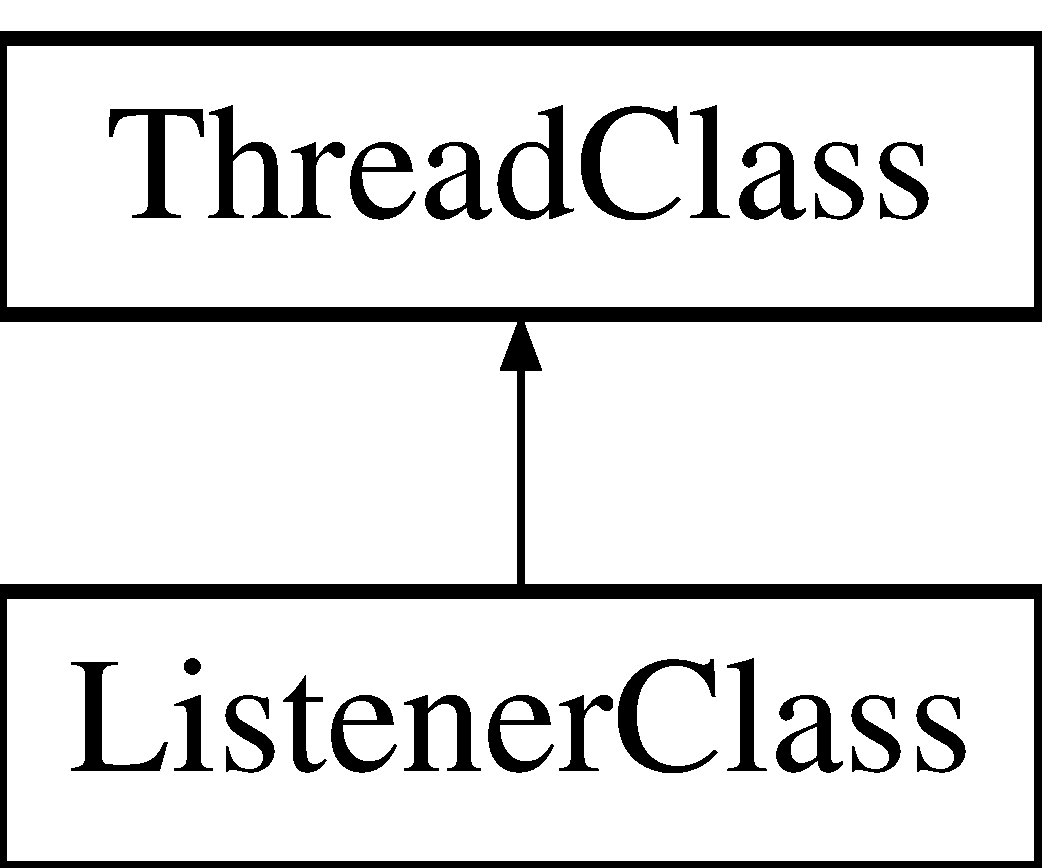
\includegraphics[height=2.000000cm]{classListenerClass}
\end{center}
\end{figure}
\subsection*{\-Public \-Member \-Functions}
\begin{DoxyCompactItemize}
\item 
\hyperlink{classListenerClass_a51123fb7fefe03fb4dcd347fab7d53e9}{\-Listener\-Class} (int, int, int)
\item 
void \hyperlink{classListenerClass_a1ea748a7a3d2af97032cb54879937a7b}{handle\-Connection} (int)
\item 
\hyperlink{classListenerClass_ad6ca9ef2ec7d0f5dc1c41c629b62ad62}{$\sim$\-Listener\-Class} ()
\item 
void \hyperlink{classListenerClass_a928179045e95f0b175ce895dbb8cbafd}{set\-Status} (int)
\item 
int \hyperlink{classListenerClass_a2af2bac82ab30eda5ef876e6f4c04df1}{users\-Connected} ()
\item 
std\-::string \hyperlink{classListenerClass_a7d698e794f88524ceb2a01f7b8885431}{available\-Channels} ()
\end{DoxyCompactItemize}
\subsection*{\-Private \-Member \-Functions}
\begin{DoxyCompactItemize}
\item 
void \hyperlink{classListenerClass_a3c03db442f150655fb00cc5b562f4cc8}{\-Setup} ()
\item 
void \hyperlink{classListenerClass_ac8dd8fe72b34ab5412f8ffe1fec18808}{\-Execute} (void $\ast$)
\end{DoxyCompactItemize}
\subsection*{\-Private \-Attributes}
\begin{DoxyCompactItemize}
\item 
int \hyperlink{classListenerClass_aa89d7f1e7689480cba000b3c0fa8b6c2}{incoming\-F\-D}
\item 
int \hyperlink{classListenerClass_a893af73361a8309146dd32f2ea25ad84}{max\-Selectors}
\item 
int \hyperlink{classListenerClass_ac7e26fe8e0be92e2f3a789bec5ef0769}{status}
\item 
int \hyperlink{classListenerClass_a549253403e548ddd2686076affd5ec94}{queue}
\item 
int \hyperlink{classListenerClass_a12f33aca6bb74c05fc425e0a95b43ed7}{port}
\item 
std\-::map$<$ std\-::string, \-Channel $\ast$ $>$ \hyperlink{classListenerClass_a117b3a05516645559a9d2ebfc59e402d}{channels}
\item 
\-Connections\-Waiting \hyperlink{classListenerClass_a042f0c9bc8ae4ea89fdf667cac503362}{connections\-Waiting}
\item 
\-Channel\-Selector $\ast$$\ast$ \hyperlink{classListenerClass_a464fae6bbe88763173d475959707a9ce}{chselect}
\item 
\hyperlink{classSQLite}{\-S\-Q\-Lite} \hyperlink{classListenerClass_ab12f05f1fd420de2c5af04a7ecbeba4d}{app\-D\-B}
\item 
\hyperlink{classTCPListener}{\-T\-C\-P\-Listener} \hyperlink{classListenerClass_abf5a4811e19cc0c23a3cdcc08f43a09f}{listener\-Socket}
\end{DoxyCompactItemize}


\subsection{\-Constructor \& \-Destructor \-Documentation}
\hypertarget{classListenerClass_a51123fb7fefe03fb4dcd347fab7d53e9}{\index{\-Listener\-Class@{\-Listener\-Class}!\-Listener\-Class@{\-Listener\-Class}}
\index{\-Listener\-Class@{\-Listener\-Class}!ListenerClass@{\-Listener\-Class}}
\subsubsection[{\-Listener\-Class}]{\setlength{\rightskip}{0pt plus 5cm}{\bf \-Listener\-Class\-::\-Listener\-Class} (
\begin{DoxyParamCaption}
\item[{int}]{port, }
\item[{int}]{queue, }
\item[{int}]{selectors}
\end{DoxyParamCaption}
)}}\label{classListenerClass_a51123fb7fefe03fb4dcd347fab7d53e9}
\hypertarget{classListenerClass_ad6ca9ef2ec7d0f5dc1c41c629b62ad62}{\index{\-Listener\-Class@{\-Listener\-Class}!$\sim$\-Listener\-Class@{$\sim$\-Listener\-Class}}
\index{$\sim$\-Listener\-Class@{$\sim$\-Listener\-Class}!ListenerClass@{\-Listener\-Class}}
\subsubsection[{$\sim$\-Listener\-Class}]{\setlength{\rightskip}{0pt plus 5cm}{\bf \-Listener\-Class\-::$\sim$\-Listener\-Class} (
\begin{DoxyParamCaption}
{}
\end{DoxyParamCaption}
)}}\label{classListenerClass_ad6ca9ef2ec7d0f5dc1c41c629b62ad62}


\subsection{\-Member \-Function \-Documentation}
\hypertarget{classListenerClass_a7d698e794f88524ceb2a01f7b8885431}{\index{\-Listener\-Class@{\-Listener\-Class}!available\-Channels@{available\-Channels}}
\index{available\-Channels@{available\-Channels}!ListenerClass@{\-Listener\-Class}}
\subsubsection[{available\-Channels}]{\setlength{\rightskip}{0pt plus 5cm}std\-::string {\bf \-Listener\-Class\-::available\-Channels} (
\begin{DoxyParamCaption}
{}
\end{DoxyParamCaption}
)}}\label{classListenerClass_a7d698e794f88524ceb2a01f7b8885431}
\hypertarget{classListenerClass_ac8dd8fe72b34ab5412f8ffe1fec18808}{\index{\-Listener\-Class@{\-Listener\-Class}!\-Execute@{\-Execute}}
\index{\-Execute@{\-Execute}!ListenerClass@{\-Listener\-Class}}
\subsubsection[{\-Execute}]{\setlength{\rightskip}{0pt plus 5cm}void {\bf \-Listener\-Class\-::\-Execute} (
\begin{DoxyParamCaption}
\item[{void $\ast$}]{arg}
\end{DoxyParamCaption}
)\hspace{0.3cm}{\ttfamily  \mbox{[}private, virtual\mbox{]}}}}\label{classListenerClass_ac8dd8fe72b34ab5412f8ffe1fec18808}


\-Implements \hyperlink{classThreadClass_aa6b3fb3567bd8b7d67b4aa200cd47e00}{\-Thread\-Class}.

\hypertarget{classListenerClass_a1ea748a7a3d2af97032cb54879937a7b}{\index{\-Listener\-Class@{\-Listener\-Class}!handle\-Connection@{handle\-Connection}}
\index{handle\-Connection@{handle\-Connection}!ListenerClass@{\-Listener\-Class}}
\subsubsection[{handle\-Connection}]{\setlength{\rightskip}{0pt plus 5cm}void {\bf \-Listener\-Class\-::handle\-Connection} (
\begin{DoxyParamCaption}
\item[{int}]{desc}
\end{DoxyParamCaption}
)}}\label{classListenerClass_a1ea748a7a3d2af97032cb54879937a7b}
\hypertarget{classListenerClass_a928179045e95f0b175ce895dbb8cbafd}{\index{\-Listener\-Class@{\-Listener\-Class}!set\-Status@{set\-Status}}
\index{set\-Status@{set\-Status}!ListenerClass@{\-Listener\-Class}}
\subsubsection[{set\-Status}]{\setlength{\rightskip}{0pt plus 5cm}void {\bf \-Listener\-Class\-::set\-Status} (
\begin{DoxyParamCaption}
\item[{int}]{s}
\end{DoxyParamCaption}
)}}\label{classListenerClass_a928179045e95f0b175ce895dbb8cbafd}
\hypertarget{classListenerClass_a3c03db442f150655fb00cc5b562f4cc8}{\index{\-Listener\-Class@{\-Listener\-Class}!\-Setup@{\-Setup}}
\index{\-Setup@{\-Setup}!ListenerClass@{\-Listener\-Class}}
\subsubsection[{\-Setup}]{\setlength{\rightskip}{0pt plus 5cm}void {\bf \-Listener\-Class\-::\-Setup} (
\begin{DoxyParamCaption}
{}
\end{DoxyParamCaption}
)\hspace{0.3cm}{\ttfamily  \mbox{[}private, virtual\mbox{]}}}}\label{classListenerClass_a3c03db442f150655fb00cc5b562f4cc8}


\-Implements \hyperlink{classThreadClass_a79775d1799a12bf4c9575cad8fd462d0}{\-Thread\-Class}.

\hypertarget{classListenerClass_a2af2bac82ab30eda5ef876e6f4c04df1}{\index{\-Listener\-Class@{\-Listener\-Class}!users\-Connected@{users\-Connected}}
\index{users\-Connected@{users\-Connected}!ListenerClass@{\-Listener\-Class}}
\subsubsection[{users\-Connected}]{\setlength{\rightskip}{0pt plus 5cm}int {\bf \-Listener\-Class\-::users\-Connected} (
\begin{DoxyParamCaption}
{}
\end{DoxyParamCaption}
)}}\label{classListenerClass_a2af2bac82ab30eda5ef876e6f4c04df1}


\subsection{\-Field \-Documentation}
\hypertarget{classListenerClass_ab12f05f1fd420de2c5af04a7ecbeba4d}{\index{\-Listener\-Class@{\-Listener\-Class}!app\-D\-B@{app\-D\-B}}
\index{app\-D\-B@{app\-D\-B}!ListenerClass@{\-Listener\-Class}}
\subsubsection[{app\-D\-B}]{\setlength{\rightskip}{0pt plus 5cm}{\bf \-S\-Q\-Lite} {\bf \-Listener\-Class\-::app\-D\-B}\hspace{0.3cm}{\ttfamily  \mbox{[}private\mbox{]}}}}\label{classListenerClass_ab12f05f1fd420de2c5af04a7ecbeba4d}
\hypertarget{classListenerClass_a117b3a05516645559a9d2ebfc59e402d}{\index{\-Listener\-Class@{\-Listener\-Class}!channels@{channels}}
\index{channels@{channels}!ListenerClass@{\-Listener\-Class}}
\subsubsection[{channels}]{\setlength{\rightskip}{0pt plus 5cm}std\-::map$<$std\-::string, \-Channel$\ast$$>$ {\bf \-Listener\-Class\-::channels}\hspace{0.3cm}{\ttfamily  \mbox{[}private\mbox{]}}}}\label{classListenerClass_a117b3a05516645559a9d2ebfc59e402d}
\hypertarget{classListenerClass_a464fae6bbe88763173d475959707a9ce}{\index{\-Listener\-Class@{\-Listener\-Class}!chselect@{chselect}}
\index{chselect@{chselect}!ListenerClass@{\-Listener\-Class}}
\subsubsection[{chselect}]{\setlength{\rightskip}{0pt plus 5cm}\-Channel\-Selector$\ast$$\ast$ {\bf \-Listener\-Class\-::chselect}\hspace{0.3cm}{\ttfamily  \mbox{[}private\mbox{]}}}}\label{classListenerClass_a464fae6bbe88763173d475959707a9ce}
\hypertarget{classListenerClass_a042f0c9bc8ae4ea89fdf667cac503362}{\index{\-Listener\-Class@{\-Listener\-Class}!connections\-Waiting@{connections\-Waiting}}
\index{connections\-Waiting@{connections\-Waiting}!ListenerClass@{\-Listener\-Class}}
\subsubsection[{connections\-Waiting}]{\setlength{\rightskip}{0pt plus 5cm}\-Connections\-Waiting {\bf \-Listener\-Class\-::connections\-Waiting}\hspace{0.3cm}{\ttfamily  \mbox{[}private\mbox{]}}}}\label{classListenerClass_a042f0c9bc8ae4ea89fdf667cac503362}
\hypertarget{classListenerClass_aa89d7f1e7689480cba000b3c0fa8b6c2}{\index{\-Listener\-Class@{\-Listener\-Class}!incoming\-F\-D@{incoming\-F\-D}}
\index{incoming\-F\-D@{incoming\-F\-D}!ListenerClass@{\-Listener\-Class}}
\subsubsection[{incoming\-F\-D}]{\setlength{\rightskip}{0pt plus 5cm}int {\bf \-Listener\-Class\-::incoming\-F\-D}\hspace{0.3cm}{\ttfamily  \mbox{[}private\mbox{]}}}}\label{classListenerClass_aa89d7f1e7689480cba000b3c0fa8b6c2}
\hypertarget{classListenerClass_abf5a4811e19cc0c23a3cdcc08f43a09f}{\index{\-Listener\-Class@{\-Listener\-Class}!listener\-Socket@{listener\-Socket}}
\index{listener\-Socket@{listener\-Socket}!ListenerClass@{\-Listener\-Class}}
\subsubsection[{listener\-Socket}]{\setlength{\rightskip}{0pt plus 5cm}{\bf \-T\-C\-P\-Listener} {\bf \-Listener\-Class\-::listener\-Socket}\hspace{0.3cm}{\ttfamily  \mbox{[}private\mbox{]}}}}\label{classListenerClass_abf5a4811e19cc0c23a3cdcc08f43a09f}
\hypertarget{classListenerClass_a893af73361a8309146dd32f2ea25ad84}{\index{\-Listener\-Class@{\-Listener\-Class}!max\-Selectors@{max\-Selectors}}
\index{max\-Selectors@{max\-Selectors}!ListenerClass@{\-Listener\-Class}}
\subsubsection[{max\-Selectors}]{\setlength{\rightskip}{0pt plus 5cm}int {\bf \-Listener\-Class\-::max\-Selectors}\hspace{0.3cm}{\ttfamily  \mbox{[}private\mbox{]}}}}\label{classListenerClass_a893af73361a8309146dd32f2ea25ad84}
\hypertarget{classListenerClass_a12f33aca6bb74c05fc425e0a95b43ed7}{\index{\-Listener\-Class@{\-Listener\-Class}!port@{port}}
\index{port@{port}!ListenerClass@{\-Listener\-Class}}
\subsubsection[{port}]{\setlength{\rightskip}{0pt plus 5cm}int {\bf \-Listener\-Class\-::port}\hspace{0.3cm}{\ttfamily  \mbox{[}private\mbox{]}}}}\label{classListenerClass_a12f33aca6bb74c05fc425e0a95b43ed7}
\hypertarget{classListenerClass_a549253403e548ddd2686076affd5ec94}{\index{\-Listener\-Class@{\-Listener\-Class}!queue@{queue}}
\index{queue@{queue}!ListenerClass@{\-Listener\-Class}}
\subsubsection[{queue}]{\setlength{\rightskip}{0pt plus 5cm}int {\bf \-Listener\-Class\-::queue}\hspace{0.3cm}{\ttfamily  \mbox{[}private\mbox{]}}}}\label{classListenerClass_a549253403e548ddd2686076affd5ec94}
\hypertarget{classListenerClass_ac7e26fe8e0be92e2f3a789bec5ef0769}{\index{\-Listener\-Class@{\-Listener\-Class}!status@{status}}
\index{status@{status}!ListenerClass@{\-Listener\-Class}}
\subsubsection[{status}]{\setlength{\rightskip}{0pt plus 5cm}int {\bf \-Listener\-Class\-::status}\hspace{0.3cm}{\ttfamily  \mbox{[}private\mbox{]}}}}\label{classListenerClass_ac7e26fe8e0be92e2f3a789bec5ef0769}


\-The documentation for this class was generated from the following files\-:\begin{DoxyCompactItemize}
\item 
\hyperlink{ListenerClass_8h}{\-Listener\-Class.\-h}\item 
\hyperlink{ListenerClass_8cpp}{\-Listener\-Class.\-cpp}\end{DoxyCompactItemize}

\hypertarget{classLockClass}{\section{\-Lock\-Class \-Class \-Reference}
\label{classLockClass}\index{\-Lock\-Class@{\-Lock\-Class}}
}


{\ttfamily \#include $<$\-Lock\-Class.\-h$>$}

\subsection*{\-Public \-Member \-Functions}
\begin{DoxyCompactItemize}
\item 
\hyperlink{classLockClass_a6baa4ddfe723e4a952479618befb44dd}{\-Lock\-Class} ()
\item 
\hyperlink{classLockClass_adfda270770c8e6a7732b5af9816dadd1}{$\sim$\-Lock\-Class} ()
\item 
void \hyperlink{classLockClass_aab284bd73f4c67bf75c8a5915431cf6e}{lock} ()
\item 
void \hyperlink{classLockClass_a85e58911b6d3f48b0d7660cf1f04cadb}{unlock} ()
\end{DoxyCompactItemize}
\subsection*{\-Private \-Attributes}
\begin{DoxyCompactItemize}
\item 
pthread\-\_\-mutex\-\_\-t \hyperlink{classLockClass_a9205b3be1c788ef9f091a71e7c94ccbe}{plock}
\end{DoxyCompactItemize}


\subsection{\-Constructor \& \-Destructor \-Documentation}
\hypertarget{classLockClass_a6baa4ddfe723e4a952479618befb44dd}{\index{\-Lock\-Class@{\-Lock\-Class}!\-Lock\-Class@{\-Lock\-Class}}
\index{\-Lock\-Class@{\-Lock\-Class}!LockClass@{\-Lock\-Class}}
\subsubsection[{\-Lock\-Class}]{\setlength{\rightskip}{0pt plus 5cm}{\bf \-Lock\-Class\-::\-Lock\-Class} (
\begin{DoxyParamCaption}
{}
\end{DoxyParamCaption}
)}}\label{classLockClass_a6baa4ddfe723e4a952479618befb44dd}
\hypertarget{classLockClass_adfda270770c8e6a7732b5af9816dadd1}{\index{\-Lock\-Class@{\-Lock\-Class}!$\sim$\-Lock\-Class@{$\sim$\-Lock\-Class}}
\index{$\sim$\-Lock\-Class@{$\sim$\-Lock\-Class}!LockClass@{\-Lock\-Class}}
\subsubsection[{$\sim$\-Lock\-Class}]{\setlength{\rightskip}{0pt plus 5cm}{\bf \-Lock\-Class\-::$\sim$\-Lock\-Class} (
\begin{DoxyParamCaption}
{}
\end{DoxyParamCaption}
)}}\label{classLockClass_adfda270770c8e6a7732b5af9816dadd1}


\subsection{\-Member \-Function \-Documentation}
\hypertarget{classLockClass_aab284bd73f4c67bf75c8a5915431cf6e}{\index{\-Lock\-Class@{\-Lock\-Class}!lock@{lock}}
\index{lock@{lock}!LockClass@{\-Lock\-Class}}
\subsubsection[{lock}]{\setlength{\rightskip}{0pt plus 5cm}void {\bf \-Lock\-Class\-::lock} (
\begin{DoxyParamCaption}
{}
\end{DoxyParamCaption}
)}}\label{classLockClass_aab284bd73f4c67bf75c8a5915431cf6e}
\hypertarget{classLockClass_a85e58911b6d3f48b0d7660cf1f04cadb}{\index{\-Lock\-Class@{\-Lock\-Class}!unlock@{unlock}}
\index{unlock@{unlock}!LockClass@{\-Lock\-Class}}
\subsubsection[{unlock}]{\setlength{\rightskip}{0pt plus 5cm}void {\bf \-Lock\-Class\-::unlock} (
\begin{DoxyParamCaption}
{}
\end{DoxyParamCaption}
)}}\label{classLockClass_a85e58911b6d3f48b0d7660cf1f04cadb}


\subsection{\-Field \-Documentation}
\hypertarget{classLockClass_a9205b3be1c788ef9f091a71e7c94ccbe}{\index{\-Lock\-Class@{\-Lock\-Class}!plock@{plock}}
\index{plock@{plock}!LockClass@{\-Lock\-Class}}
\subsubsection[{plock}]{\setlength{\rightskip}{0pt plus 5cm}pthread\-\_\-mutex\-\_\-t {\bf \-Lock\-Class\-::plock}\hspace{0.3cm}{\ttfamily  \mbox{[}private\mbox{]}}}}\label{classLockClass_a9205b3be1c788ef9f091a71e7c94ccbe}


\-The documentation for this class was generated from the following files\-:\begin{DoxyCompactItemize}
\item 
common/\hyperlink{LockClass_8h}{\-Lock\-Class.\-h}\item 
common/\hyperlink{LockClass_8cpp}{\-Lock\-Class.\-cpp}\end{DoxyCompactItemize}

\hypertarget{classLogger}{\section{\-Logger \-Class \-Reference}
\label{classLogger}\index{\-Logger@{\-Logger}}
}


{\ttfamily \#include $<$\-Logger.\-h$>$}

\subsection*{\-Public \-Member \-Functions}
\begin{DoxyCompactItemize}
\item 
\hyperlink{classLogger_acb668a9e186a25fbaad2e4af6d1ed00a}{$\sim$\-Logger} ()
\item 
void \hyperlink{classLogger_a61691525efbcb21337e37b28bcedc982}{print} (\hyperlink{Logger_8h_a37601483630df382986fba4887e536bd}{\-Log\-String})
\end{DoxyCompactItemize}
\subsection*{\-Static \-Public \-Member \-Functions}
\begin{DoxyCompactItemize}
\item 
static \hyperlink{classLogger}{\-Logger} $\ast$ \hyperlink{classLogger_afae0bf19389387a916656073572cb846}{\-Instance} ()
\end{DoxyCompactItemize}
\subsection*{\-Private \-Member \-Functions}
\begin{DoxyCompactItemize}
\item 
\hyperlink{classLogger_abc41bfb031d896170c7675fa96a6b30c}{\-Logger} ()
\item 
\hyperlink{classLogger_a21340fb1037a0f71c0dc659ea33678a4}{\-Logger} (\hyperlink{classLogger}{\-Logger} const \&)
\item 
\hyperlink{classLogger}{\-Logger} \& \hyperlink{classLogger_a26fa369e27132ca4bf478710919f6e70}{operator=} (\hyperlink{classLogger}{\-Logger} const \&)
\end{DoxyCompactItemize}
\subsection*{\-Static \-Private \-Attributes}
\begin{DoxyCompactItemize}
\item 
static \hyperlink{classLogger}{\-Logger} $\ast$ \hyperlink{classLogger_a1b2d5c8754e1f4f5aca49e75b0c8357c}{m\-\_\-\-Instance} = \-N\-U\-L\-L
\end{DoxyCompactItemize}


\subsection{\-Constructor \& \-Destructor \-Documentation}
\hypertarget{classLogger_acb668a9e186a25fbaad2e4af6d1ed00a}{\index{\-Logger@{\-Logger}!$\sim$\-Logger@{$\sim$\-Logger}}
\index{$\sim$\-Logger@{$\sim$\-Logger}!Logger@{\-Logger}}
\subsubsection[{$\sim$\-Logger}]{\setlength{\rightskip}{0pt plus 5cm}{\bf \-Logger\-::$\sim$\-Logger} (
\begin{DoxyParamCaption}
{}
\end{DoxyParamCaption}
)}}\label{classLogger_acb668a9e186a25fbaad2e4af6d1ed00a}
\hypertarget{classLogger_abc41bfb031d896170c7675fa96a6b30c}{\index{\-Logger@{\-Logger}!\-Logger@{\-Logger}}
\index{\-Logger@{\-Logger}!Logger@{\-Logger}}
\subsubsection[{\-Logger}]{\setlength{\rightskip}{0pt plus 5cm}{\bf \-Logger\-::\-Logger} (
\begin{DoxyParamCaption}
{}
\end{DoxyParamCaption}
)\hspace{0.3cm}{\ttfamily  \mbox{[}inline, private\mbox{]}}}}\label{classLogger_abc41bfb031d896170c7675fa96a6b30c}
\hypertarget{classLogger_a21340fb1037a0f71c0dc659ea33678a4}{\index{\-Logger@{\-Logger}!\-Logger@{\-Logger}}
\index{\-Logger@{\-Logger}!Logger@{\-Logger}}
\subsubsection[{\-Logger}]{\setlength{\rightskip}{0pt plus 5cm}{\bf \-Logger\-::\-Logger} (
\begin{DoxyParamCaption}
\item[{{\bf \-Logger} const \&}]{}
\end{DoxyParamCaption}
)\hspace{0.3cm}{\ttfamily  \mbox{[}inline, private\mbox{]}}}}\label{classLogger_a21340fb1037a0f71c0dc659ea33678a4}


\subsection{\-Member \-Function \-Documentation}
\hypertarget{classLogger_afae0bf19389387a916656073572cb846}{\index{\-Logger@{\-Logger}!\-Instance@{\-Instance}}
\index{\-Instance@{\-Instance}!Logger@{\-Logger}}
\subsubsection[{\-Instance}]{\setlength{\rightskip}{0pt plus 5cm}{\bf \-Logger} $\ast$ {\bf \-Logger\-::\-Instance} (
\begin{DoxyParamCaption}
{}
\end{DoxyParamCaption}
)\hspace{0.3cm}{\ttfamily  \mbox{[}static\mbox{]}}}}\label{classLogger_afae0bf19389387a916656073572cb846}
\hypertarget{classLogger_a26fa369e27132ca4bf478710919f6e70}{\index{\-Logger@{\-Logger}!operator=@{operator=}}
\index{operator=@{operator=}!Logger@{\-Logger}}
\subsubsection[{operator=}]{\setlength{\rightskip}{0pt plus 5cm}{\bf \-Logger}\& \-Logger\-::operator= (
\begin{DoxyParamCaption}
\item[{{\bf \-Logger} const \&}]{}
\end{DoxyParamCaption}
)\hspace{0.3cm}{\ttfamily  \mbox{[}inline, private\mbox{]}}}}\label{classLogger_a26fa369e27132ca4bf478710919f6e70}
\hypertarget{classLogger_a61691525efbcb21337e37b28bcedc982}{\index{\-Logger@{\-Logger}!print@{print}}
\index{print@{print}!Logger@{\-Logger}}
\subsubsection[{print}]{\setlength{\rightskip}{0pt plus 5cm}void {\bf \-Logger\-::print} (
\begin{DoxyParamCaption}
\item[{{\bf \-Log\-String}}]{output}
\end{DoxyParamCaption}
)}}\label{classLogger_a61691525efbcb21337e37b28bcedc982}


\subsection{\-Field \-Documentation}
\hypertarget{classLogger_a1b2d5c8754e1f4f5aca49e75b0c8357c}{\index{\-Logger@{\-Logger}!m\-\_\-\-Instance@{m\-\_\-\-Instance}}
\index{m\-\_\-\-Instance@{m\-\_\-\-Instance}!Logger@{\-Logger}}
\subsubsection[{m\-\_\-\-Instance}]{\setlength{\rightskip}{0pt plus 5cm}{\bf \-Logger} $\ast$ {\bf \-Logger\-::m\-\_\-\-Instance} = \-N\-U\-L\-L\hspace{0.3cm}{\ttfamily  \mbox{[}static, private\mbox{]}}}}\label{classLogger_a1b2d5c8754e1f4f5aca49e75b0c8357c}


\-The documentation for this class was generated from the following files\-:\begin{DoxyCompactItemize}
\item 
common/\hyperlink{Logger_8h}{\-Logger.\-h}\item 
common/\hyperlink{Logger_8cpp}{\-Logger.\-cpp}\end{DoxyCompactItemize}

\hypertarget{classLua__State}{\section{\-Lua\-\_\-\-State \-Class \-Reference}
\label{classLua__State}\index{\-Lua\-\_\-\-State@{\-Lua\-\_\-\-State}}
}


{\ttfamily \#include $<$\-Script\-Loader.\-h$>$}

\subsection*{\-Public \-Member \-Functions}
\begin{DoxyCompactItemize}
\item 
\hyperlink{classLua__State_aa0b203e648c90666e79a5a417736932d}{\-Lua\-\_\-\-State} ()
\item 
\hyperlink{classLua__State_a33c6e11ea283e46205fbe8d0f3f8172b}{$\sim$\-Lua\-\_\-\-State} ()
\item 
\hyperlink{classLua__State_aca3de033478261d6b9850b7f09e76d2b}{operator lua\-\_\-\-State $\ast$} ()
\end{DoxyCompactItemize}
\subsection*{\-Private \-Attributes}
\begin{DoxyCompactItemize}
\item 
lua\-\_\-\-State $\ast$ \hyperlink{classLua__State_adf1bf0d484862b5cbe63ba5215fdc498}{\-L}
\end{DoxyCompactItemize}


\subsection{\-Constructor \& \-Destructor \-Documentation}
\hypertarget{classLua__State_aa0b203e648c90666e79a5a417736932d}{\index{\-Lua\-\_\-\-State@{\-Lua\-\_\-\-State}!\-Lua\-\_\-\-State@{\-Lua\-\_\-\-State}}
\index{\-Lua\-\_\-\-State@{\-Lua\-\_\-\-State}!Lua_State@{\-Lua\-\_\-\-State}}
\subsubsection[{\-Lua\-\_\-\-State}]{\setlength{\rightskip}{0pt plus 5cm}{\bf \-Lua\-\_\-\-State\-::\-Lua\-\_\-\-State} (
\begin{DoxyParamCaption}
{}
\end{DoxyParamCaption}
)\hspace{0.3cm}{\ttfamily  \mbox{[}inline\mbox{]}}}}\label{classLua__State_aa0b203e648c90666e79a5a417736932d}
\hypertarget{classLua__State_a33c6e11ea283e46205fbe8d0f3f8172b}{\index{\-Lua\-\_\-\-State@{\-Lua\-\_\-\-State}!$\sim$\-Lua\-\_\-\-State@{$\sim$\-Lua\-\_\-\-State}}
\index{$\sim$\-Lua\-\_\-\-State@{$\sim$\-Lua\-\_\-\-State}!Lua_State@{\-Lua\-\_\-\-State}}
\subsubsection[{$\sim$\-Lua\-\_\-\-State}]{\setlength{\rightskip}{0pt plus 5cm}{\bf \-Lua\-\_\-\-State\-::$\sim$\-Lua\-\_\-\-State} (
\begin{DoxyParamCaption}
{}
\end{DoxyParamCaption}
)\hspace{0.3cm}{\ttfamily  \mbox{[}inline\mbox{]}}}}\label{classLua__State_a33c6e11ea283e46205fbe8d0f3f8172b}


\subsection{\-Member \-Function \-Documentation}
\hypertarget{classLua__State_aca3de033478261d6b9850b7f09e76d2b}{\index{\-Lua\-\_\-\-State@{\-Lua\-\_\-\-State}!operator lua\-\_\-\-State $\ast$@{operator lua\-\_\-\-State $\ast$}}
\index{operator lua\-\_\-\-State $\ast$@{operator lua\-\_\-\-State $\ast$}!Lua_State@{\-Lua\-\_\-\-State}}
\subsubsection[{operator lua\-\_\-\-State $\ast$}]{\setlength{\rightskip}{0pt plus 5cm}\-Lua\-\_\-\-State\-::operator lua\-\_\-\-State $\ast$ (
\begin{DoxyParamCaption}
{}
\end{DoxyParamCaption}
)\hspace{0.3cm}{\ttfamily  \mbox{[}inline\mbox{]}}}}\label{classLua__State_aca3de033478261d6b9850b7f09e76d2b}


\subsection{\-Field \-Documentation}
\hypertarget{classLua__State_adf1bf0d484862b5cbe63ba5215fdc498}{\index{\-Lua\-\_\-\-State@{\-Lua\-\_\-\-State}!\-L@{\-L}}
\index{\-L@{\-L}!Lua_State@{\-Lua\-\_\-\-State}}
\subsubsection[{\-L}]{\setlength{\rightskip}{0pt plus 5cm}lua\-\_\-\-State$\ast$ {\bf \-Lua\-\_\-\-State\-::\-L}\hspace{0.3cm}{\ttfamily  \mbox{[}private\mbox{]}}}}\label{classLua__State_adf1bf0d484862b5cbe63ba5215fdc498}


\-The documentation for this class was generated from the following file\-:\begin{DoxyCompactItemize}
\item 
scriptloader/\hyperlink{ScriptLoader_8h}{\-Script\-Loader.\-h}\end{DoxyCompactItemize}

\hypertarget{classScriptLoader}{\section{\-Script\-Loader \-Class \-Reference}
\label{classScriptLoader}\index{\-Script\-Loader@{\-Script\-Loader}}
}


{\ttfamily \#include $<$\-Script\-Loader.\-h$>$}

\subsection*{\-Public \-Member \-Functions}
\begin{DoxyCompactItemize}
\item 
\hyperlink{classScriptLoader_a78a02f536324e70296d2a3145422a995}{\-Script\-Loader} ()
\item 
\hyperlink{classScriptLoader_a27ee182ec99bae44d69c0f4395a74627}{$\sim$\-Script\-Loader} ()
\item 
int \hyperlink{classScriptLoader_a9086035942d48d0e2e3f27adf6e64610}{load} (std\-::string)
\item 
int \hyperlink{classScriptLoader_ad6d0c9a988d5672ba4e7dd6c21b42087}{load\-Text} (std\-::string)
\item 
int \hyperlink{classScriptLoader_a7ca17e7aed24fc73154558b79fe6230c}{load\-Lib} (std\-::string)
\item 
int \hyperlink{classScriptLoader_aeed89cb2b229db62e45a0a546fe97802}{add\-Proc} (lua\-\_\-\-C\-Function, void $\ast$, const std\-::string)
\item 
void \hyperlink{classScriptLoader_a96305ed715530eff1b5f5b82f324dbe2}{call} (std\-::string)
\item 
void \hyperlink{classScriptLoader_aa776dfca1106ee9f713850eacabe8a13}{call} (std\-::string, \hyperlink{ScriptLoader_8h_a46a39c227bfcf3a06bd727417f54feef}{\-S\-L\-Arg})
\end{DoxyCompactItemize}
\subsection*{\-Private \-Attributes}
\begin{DoxyCompactItemize}
\item 
\hyperlink{classLua__State}{\-Lua\-\_\-\-State} \hyperlink{classScriptLoader_a2c3fcbd1aa0d7db987b51d1c68e02c06}{state}
\end{DoxyCompactItemize}


\subsection{\-Constructor \& \-Destructor \-Documentation}
\hypertarget{classScriptLoader_a78a02f536324e70296d2a3145422a995}{\index{\-Script\-Loader@{\-Script\-Loader}!\-Script\-Loader@{\-Script\-Loader}}
\index{\-Script\-Loader@{\-Script\-Loader}!ScriptLoader@{\-Script\-Loader}}
\subsubsection[{\-Script\-Loader}]{\setlength{\rightskip}{0pt plus 5cm}{\bf \-Script\-Loader\-::\-Script\-Loader} (
\begin{DoxyParamCaption}
{}
\end{DoxyParamCaption}
)}}\label{classScriptLoader_a78a02f536324e70296d2a3145422a995}
\hypertarget{classScriptLoader_a27ee182ec99bae44d69c0f4395a74627}{\index{\-Script\-Loader@{\-Script\-Loader}!$\sim$\-Script\-Loader@{$\sim$\-Script\-Loader}}
\index{$\sim$\-Script\-Loader@{$\sim$\-Script\-Loader}!ScriptLoader@{\-Script\-Loader}}
\subsubsection[{$\sim$\-Script\-Loader}]{\setlength{\rightskip}{0pt plus 5cm}{\bf \-Script\-Loader\-::$\sim$\-Script\-Loader} (
\begin{DoxyParamCaption}
{}
\end{DoxyParamCaption}
)}}\label{classScriptLoader_a27ee182ec99bae44d69c0f4395a74627}


\subsection{\-Member \-Function \-Documentation}
\hypertarget{classScriptLoader_aeed89cb2b229db62e45a0a546fe97802}{\index{\-Script\-Loader@{\-Script\-Loader}!add\-Proc@{add\-Proc}}
\index{add\-Proc@{add\-Proc}!ScriptLoader@{\-Script\-Loader}}
\subsubsection[{add\-Proc}]{\setlength{\rightskip}{0pt plus 5cm}int {\bf \-Script\-Loader\-::add\-Proc} (
\begin{DoxyParamCaption}
\item[{lua\-\_\-\-C\-Function}]{fn, }
\item[{void $\ast$}]{arg, }
\item[{const std\-::string}]{fn\-\_\-name}
\end{DoxyParamCaption}
)}}\label{classScriptLoader_aeed89cb2b229db62e45a0a546fe97802}
\hypertarget{classScriptLoader_a96305ed715530eff1b5f5b82f324dbe2}{\index{\-Script\-Loader@{\-Script\-Loader}!call@{call}}
\index{call@{call}!ScriptLoader@{\-Script\-Loader}}
\subsubsection[{call}]{\setlength{\rightskip}{0pt plus 5cm}void {\bf \-Script\-Loader\-::call} (
\begin{DoxyParamCaption}
\item[{std\-::string}]{func\-\_\-name}
\end{DoxyParamCaption}
)}}\label{classScriptLoader_a96305ed715530eff1b5f5b82f324dbe2}
\hypertarget{classScriptLoader_aa776dfca1106ee9f713850eacabe8a13}{\index{\-Script\-Loader@{\-Script\-Loader}!call@{call}}
\index{call@{call}!ScriptLoader@{\-Script\-Loader}}
\subsubsection[{call}]{\setlength{\rightskip}{0pt plus 5cm}void {\bf \-Script\-Loader\-::call} (
\begin{DoxyParamCaption}
\item[{std\-::string}]{func\-\_\-name, }
\item[{{\bf \-S\-L\-Arg}}]{args}
\end{DoxyParamCaption}
)}}\label{classScriptLoader_aa776dfca1106ee9f713850eacabe8a13}
\hypertarget{classScriptLoader_a9086035942d48d0e2e3f27adf6e64610}{\index{\-Script\-Loader@{\-Script\-Loader}!load@{load}}
\index{load@{load}!ScriptLoader@{\-Script\-Loader}}
\subsubsection[{load}]{\setlength{\rightskip}{0pt plus 5cm}int {\bf \-Script\-Loader\-::load} (
\begin{DoxyParamCaption}
\item[{std\-::string}]{filename}
\end{DoxyParamCaption}
)}}\label{classScriptLoader_a9086035942d48d0e2e3f27adf6e64610}
\hypertarget{classScriptLoader_a7ca17e7aed24fc73154558b79fe6230c}{\index{\-Script\-Loader@{\-Script\-Loader}!load\-Lib@{load\-Lib}}
\index{load\-Lib@{load\-Lib}!ScriptLoader@{\-Script\-Loader}}
\subsubsection[{load\-Lib}]{\setlength{\rightskip}{0pt plus 5cm}int {\bf \-Script\-Loader\-::load\-Lib} (
\begin{DoxyParamCaption}
\item[{std\-::string}]{filename}
\end{DoxyParamCaption}
)}}\label{classScriptLoader_a7ca17e7aed24fc73154558b79fe6230c}
\hypertarget{classScriptLoader_ad6d0c9a988d5672ba4e7dd6c21b42087}{\index{\-Script\-Loader@{\-Script\-Loader}!load\-Text@{load\-Text}}
\index{load\-Text@{load\-Text}!ScriptLoader@{\-Script\-Loader}}
\subsubsection[{load\-Text}]{\setlength{\rightskip}{0pt plus 5cm}int {\bf \-Script\-Loader\-::load\-Text} (
\begin{DoxyParamCaption}
\item[{std\-::string}]{script}
\end{DoxyParamCaption}
)}}\label{classScriptLoader_ad6d0c9a988d5672ba4e7dd6c21b42087}


\subsection{\-Field \-Documentation}
\hypertarget{classScriptLoader_a2c3fcbd1aa0d7db987b51d1c68e02c06}{\index{\-Script\-Loader@{\-Script\-Loader}!state@{state}}
\index{state@{state}!ScriptLoader@{\-Script\-Loader}}
\subsubsection[{state}]{\setlength{\rightskip}{0pt plus 5cm}{\bf \-Lua\-\_\-\-State} {\bf \-Script\-Loader\-::state}\hspace{0.3cm}{\ttfamily  \mbox{[}private\mbox{]}}}}\label{classScriptLoader_a2c3fcbd1aa0d7db987b51d1c68e02c06}


\-The documentation for this class was generated from the following files\-:\begin{DoxyCompactItemize}
\item 
scriptloader/\hyperlink{ScriptLoader_8h}{\-Script\-Loader.\-h}\item 
scriptloader/\hyperlink{ScriptLoader_8cpp}{\-Script\-Loader.\-cpp}\end{DoxyCompactItemize}

\hypertarget{classSemClass}{\section{\-Sem\-Class \-Class \-Reference}
\label{classSemClass}\index{\-Sem\-Class@{\-Sem\-Class}}
}


{\ttfamily \#include $<$\-Semaphore\-Class.\-h$>$}

\subsection*{\-Public \-Member \-Functions}
\begin{DoxyCompactItemize}
\item 
\hyperlink{classSemClass_a6704a908c6163db62f866a809ee75501}{\-Sem\-Class} ()
\item 
\hyperlink{classSemClass_a36c797b19db63037b1ad8cdcac7b85b9}{\-Sem\-Class} (unsigned int)
\item 
\hyperlink{classSemClass_a925f2f420bc62d2e5458bad046fe77ce}{$\sim$\-Sem\-Class} ()
\item 
int \hyperlink{classSemClass_a8cae9e0d23481e4dca0782045ddced00}{value} ()
\item 
int \hyperlink{classSemClass_a12aaec99fbdb8ee0879c0f99e9f71155}{wait} ()
\item 
int \hyperlink{classSemClass_a04dcd521fc7f21b93f9e07762c1010e8}{timed\-Wait} (long, time\-\_\-t)
\item 
int \hyperlink{classSemClass_a1a1a3dd0b9d3d364371036509454a24e}{post} ()
\end{DoxyCompactItemize}
\subsection*{\-Private \-Attributes}
\begin{DoxyCompactItemize}
\item 
sem\-\_\-t \hyperlink{classSemClass_a03e8d1cad1b13ab754352443cfe09d48}{s}
\end{DoxyCompactItemize}


\subsection{\-Constructor \& \-Destructor \-Documentation}
\hypertarget{classSemClass_a6704a908c6163db62f866a809ee75501}{\index{\-Sem\-Class@{\-Sem\-Class}!\-Sem\-Class@{\-Sem\-Class}}
\index{\-Sem\-Class@{\-Sem\-Class}!SemClass@{\-Sem\-Class}}
\subsubsection[{\-Sem\-Class}]{\setlength{\rightskip}{0pt plus 5cm}{\bf \-Sem\-Class\-::\-Sem\-Class} (
\begin{DoxyParamCaption}
{}
\end{DoxyParamCaption}
)}}\label{classSemClass_a6704a908c6163db62f866a809ee75501}
\hypertarget{classSemClass_a36c797b19db63037b1ad8cdcac7b85b9}{\index{\-Sem\-Class@{\-Sem\-Class}!\-Sem\-Class@{\-Sem\-Class}}
\index{\-Sem\-Class@{\-Sem\-Class}!SemClass@{\-Sem\-Class}}
\subsubsection[{\-Sem\-Class}]{\setlength{\rightskip}{0pt plus 5cm}{\bf \-Sem\-Class\-::\-Sem\-Class} (
\begin{DoxyParamCaption}
\item[{unsigned int}]{start\-Count}
\end{DoxyParamCaption}
)}}\label{classSemClass_a36c797b19db63037b1ad8cdcac7b85b9}
\hypertarget{classSemClass_a925f2f420bc62d2e5458bad046fe77ce}{\index{\-Sem\-Class@{\-Sem\-Class}!$\sim$\-Sem\-Class@{$\sim$\-Sem\-Class}}
\index{$\sim$\-Sem\-Class@{$\sim$\-Sem\-Class}!SemClass@{\-Sem\-Class}}
\subsubsection[{$\sim$\-Sem\-Class}]{\setlength{\rightskip}{0pt plus 5cm}{\bf \-Sem\-Class\-::$\sim$\-Sem\-Class} (
\begin{DoxyParamCaption}
{}
\end{DoxyParamCaption}
)}}\label{classSemClass_a925f2f420bc62d2e5458bad046fe77ce}


\subsection{\-Member \-Function \-Documentation}
\hypertarget{classSemClass_a1a1a3dd0b9d3d364371036509454a24e}{\index{\-Sem\-Class@{\-Sem\-Class}!post@{post}}
\index{post@{post}!SemClass@{\-Sem\-Class}}
\subsubsection[{post}]{\setlength{\rightskip}{0pt plus 5cm}int {\bf \-Sem\-Class\-::post} (
\begin{DoxyParamCaption}
{}
\end{DoxyParamCaption}
)}}\label{classSemClass_a1a1a3dd0b9d3d364371036509454a24e}
\hypertarget{classSemClass_a04dcd521fc7f21b93f9e07762c1010e8}{\index{\-Sem\-Class@{\-Sem\-Class}!timed\-Wait@{timed\-Wait}}
\index{timed\-Wait@{timed\-Wait}!SemClass@{\-Sem\-Class}}
\subsubsection[{timed\-Wait}]{\setlength{\rightskip}{0pt plus 5cm}int {\bf \-Sem\-Class\-::timed\-Wait} (
\begin{DoxyParamCaption}
\item[{long}]{nano\-\_\-sec, }
\item[{time\-\_\-t}]{sec}
\end{DoxyParamCaption}
)}}\label{classSemClass_a04dcd521fc7f21b93f9e07762c1010e8}
\hypertarget{classSemClass_a8cae9e0d23481e4dca0782045ddced00}{\index{\-Sem\-Class@{\-Sem\-Class}!value@{value}}
\index{value@{value}!SemClass@{\-Sem\-Class}}
\subsubsection[{value}]{\setlength{\rightskip}{0pt plus 5cm}int {\bf \-Sem\-Class\-::value} (
\begin{DoxyParamCaption}
{}
\end{DoxyParamCaption}
)}}\label{classSemClass_a8cae9e0d23481e4dca0782045ddced00}
\hypertarget{classSemClass_a12aaec99fbdb8ee0879c0f99e9f71155}{\index{\-Sem\-Class@{\-Sem\-Class}!wait@{wait}}
\index{wait@{wait}!SemClass@{\-Sem\-Class}}
\subsubsection[{wait}]{\setlength{\rightskip}{0pt plus 5cm}int {\bf \-Sem\-Class\-::wait} (
\begin{DoxyParamCaption}
{}
\end{DoxyParamCaption}
)}}\label{classSemClass_a12aaec99fbdb8ee0879c0f99e9f71155}


\subsection{\-Field \-Documentation}
\hypertarget{classSemClass_a03e8d1cad1b13ab754352443cfe09d48}{\index{\-Sem\-Class@{\-Sem\-Class}!s@{s}}
\index{s@{s}!SemClass@{\-Sem\-Class}}
\subsubsection[{s}]{\setlength{\rightskip}{0pt plus 5cm}sem\-\_\-t {\bf \-Sem\-Class\-::s}\hspace{0.3cm}{\ttfamily  \mbox{[}private\mbox{]}}}}\label{classSemClass_a03e8d1cad1b13ab754352443cfe09d48}


\-The documentation for this class was generated from the following files\-:\begin{DoxyCompactItemize}
\item 
common/\hyperlink{SemaphoreClass_8h}{\-Semaphore\-Class.\-h}\item 
common/\hyperlink{SemaphoreClass_8cpp}{\-Semaphore\-Class.\-cpp}\end{DoxyCompactItemize}

\hypertarget{classSHA1}{\section{\-S\-H\-A1 \-Class \-Reference}
\label{classSHA1}\index{\-S\-H\-A1@{\-S\-H\-A1}}
}


{\ttfamily \#include $<$sha1.\-h$>$}

\subsection*{\-Public \-Member \-Functions}
\begin{DoxyCompactItemize}
\item 
\hyperlink{classSHA1_ad49a5108ffd6996b1133bf41224ff726}{\-S\-H\-A1} ()
\item 
virtual \hyperlink{classSHA1_a8485d7c14fa29286cd3c7acfe438606d}{$\sim$\-S\-H\-A1} ()
\item 
void \hyperlink{classSHA1_accec3092d91c84d7e71d32c681357119}{\-Reset} ()
\item 
bool \hyperlink{classSHA1_ab374ecf64d54cc133805322370f3b0f1}{\-Result} (unsigned $\ast$message\-\_\-digest\-\_\-array)
\item 
void \hyperlink{classSHA1_a5612d5feb8202a4930aa271df8cbf102}{\-Input} (const unsigned char $\ast$message\-\_\-array, unsigned length)
\item 
void \hyperlink{classSHA1_a0c7555ddc781f3834c0a6218d1edc98e}{\-Input} (const char $\ast$message\-\_\-array, unsigned length)
\item 
void \hyperlink{classSHA1_af4d21901eb9ed48d8f8a16d0ec166829}{\-Input} (unsigned char message\-\_\-element)
\item 
void \hyperlink{classSHA1_a0fb5a35d1bc54e568d8774f966441c41}{\-Input} (char message\-\_\-element)
\item 
\hyperlink{classSHA1}{\-S\-H\-A1} \& \hyperlink{classSHA1_a5d334b9a7847596c51e671ae8fded37b}{operator$<$$<$} (const char $\ast$message\-\_\-array)
\item 
\hyperlink{classSHA1}{\-S\-H\-A1} \& \hyperlink{classSHA1_a4debec5cf6b08eb019c5fddb2f2ec68f}{operator$<$$<$} (const unsigned char $\ast$message\-\_\-array)
\item 
\hyperlink{classSHA1}{\-S\-H\-A1} \& \hyperlink{classSHA1_adfbd48831872d9b54bde3cd3963cfed2}{operator$<$$<$} (const char message\-\_\-element)
\item 
\hyperlink{classSHA1}{\-S\-H\-A1} \& \hyperlink{classSHA1_a52d73d41b7fc85895aadb8cea3b822ab}{operator$<$$<$} (const unsigned char message\-\_\-element)
\end{DoxyCompactItemize}
\subsection*{\-Private \-Member \-Functions}
\begin{DoxyCompactItemize}
\item 
void \hyperlink{classSHA1_a960b6f6f156144b1bd52fb20cd3d513c}{\-Process\-Message\-Block} ()
\item 
void \hyperlink{classSHA1_a1acc2aff5b7b59f5f1d3f8b89b9463a9}{\-Pad\-Message} ()
\item 
unsigned \hyperlink{classSHA1_a9b0229cb55fe2476583e0d03286250cd}{\-Circular\-Shift} (int bits, unsigned word)
\end{DoxyCompactItemize}
\subsection*{\-Private \-Attributes}
\begin{DoxyCompactItemize}
\item 
unsigned \hyperlink{classSHA1_a8a1a57e7bb77225bdd6d49fd62612d50}{\-H} \mbox{[}5\mbox{]}
\item 
unsigned \hyperlink{classSHA1_afb5ee6b8e9b99eb73e7d9f41b030d801}{\-Length\-\_\-\-Low}
\item 
unsigned \hyperlink{classSHA1_a93956884da01c8a30acc5a0a2a274730}{\-Length\-\_\-\-High}
\item 
unsigned char \hyperlink{classSHA1_a94c8fabb04fabd4604503512a4cc56a5}{\-Message\-\_\-\-Block} \mbox{[}64\mbox{]}
\item 
int \hyperlink{classSHA1_a3046d0eca31827c928c35d123db86c53}{\-Message\-\_\-\-Block\-\_\-\-Index}
\item 
bool \hyperlink{classSHA1_ae96e54267ae36ea6f2ef91f3f8fc6130}{\-Computed}
\item 
bool \hyperlink{classSHA1_a6fde29947db3aa9ef8412b8f3d1bb739}{\-Corrupted}
\end{DoxyCompactItemize}


\subsection{\-Constructor \& \-Destructor \-Documentation}
\hypertarget{classSHA1_ad49a5108ffd6996b1133bf41224ff726}{\index{\-S\-H\-A1@{\-S\-H\-A1}!\-S\-H\-A1@{\-S\-H\-A1}}
\index{\-S\-H\-A1@{\-S\-H\-A1}!SHA1@{\-S\-H\-A1}}
\subsubsection[{\-S\-H\-A1}]{\setlength{\rightskip}{0pt plus 5cm}{\bf \-S\-H\-A1\-::\-S\-H\-A1} (
\begin{DoxyParamCaption}
{}
\end{DoxyParamCaption}
)}}\label{classSHA1_ad49a5108ffd6996b1133bf41224ff726}
\hypertarget{classSHA1_a8485d7c14fa29286cd3c7acfe438606d}{\index{\-S\-H\-A1@{\-S\-H\-A1}!$\sim$\-S\-H\-A1@{$\sim$\-S\-H\-A1}}
\index{$\sim$\-S\-H\-A1@{$\sim$\-S\-H\-A1}!SHA1@{\-S\-H\-A1}}
\subsubsection[{$\sim$\-S\-H\-A1}]{\setlength{\rightskip}{0pt plus 5cm}{\bf \-S\-H\-A1\-::$\sim$\-S\-H\-A1} (
\begin{DoxyParamCaption}
{}
\end{DoxyParamCaption}
)\hspace{0.3cm}{\ttfamily  \mbox{[}virtual\mbox{]}}}}\label{classSHA1_a8485d7c14fa29286cd3c7acfe438606d}


\subsection{\-Member \-Function \-Documentation}
\hypertarget{classSHA1_a9b0229cb55fe2476583e0d03286250cd}{\index{\-S\-H\-A1@{\-S\-H\-A1}!\-Circular\-Shift@{\-Circular\-Shift}}
\index{\-Circular\-Shift@{\-Circular\-Shift}!SHA1@{\-S\-H\-A1}}
\subsubsection[{\-Circular\-Shift}]{\setlength{\rightskip}{0pt plus 5cm}unsigned {\bf \-S\-H\-A1\-::\-Circular\-Shift} (
\begin{DoxyParamCaption}
\item[{int}]{bits, }
\item[{unsigned}]{word}
\end{DoxyParamCaption}
)\hspace{0.3cm}{\ttfamily  \mbox{[}inline, private\mbox{]}}}}\label{classSHA1_a9b0229cb55fe2476583e0d03286250cd}
\hypertarget{classSHA1_a5612d5feb8202a4930aa271df8cbf102}{\index{\-S\-H\-A1@{\-S\-H\-A1}!\-Input@{\-Input}}
\index{\-Input@{\-Input}!SHA1@{\-S\-H\-A1}}
\subsubsection[{\-Input}]{\setlength{\rightskip}{0pt plus 5cm}void {\bf \-S\-H\-A1\-::\-Input} (
\begin{DoxyParamCaption}
\item[{const unsigned char $\ast$}]{message\-\_\-array, }
\item[{unsigned}]{length}
\end{DoxyParamCaption}
)}}\label{classSHA1_a5612d5feb8202a4930aa271df8cbf102}
\hypertarget{classSHA1_a0c7555ddc781f3834c0a6218d1edc98e}{\index{\-S\-H\-A1@{\-S\-H\-A1}!\-Input@{\-Input}}
\index{\-Input@{\-Input}!SHA1@{\-S\-H\-A1}}
\subsubsection[{\-Input}]{\setlength{\rightskip}{0pt plus 5cm}void {\bf \-S\-H\-A1\-::\-Input} (
\begin{DoxyParamCaption}
\item[{const char $\ast$}]{message\-\_\-array, }
\item[{unsigned}]{length}
\end{DoxyParamCaption}
)}}\label{classSHA1_a0c7555ddc781f3834c0a6218d1edc98e}
\hypertarget{classSHA1_af4d21901eb9ed48d8f8a16d0ec166829}{\index{\-S\-H\-A1@{\-S\-H\-A1}!\-Input@{\-Input}}
\index{\-Input@{\-Input}!SHA1@{\-S\-H\-A1}}
\subsubsection[{\-Input}]{\setlength{\rightskip}{0pt plus 5cm}void {\bf \-S\-H\-A1\-::\-Input} (
\begin{DoxyParamCaption}
\item[{unsigned char}]{message\-\_\-element}
\end{DoxyParamCaption}
)}}\label{classSHA1_af4d21901eb9ed48d8f8a16d0ec166829}
\hypertarget{classSHA1_a0fb5a35d1bc54e568d8774f966441c41}{\index{\-S\-H\-A1@{\-S\-H\-A1}!\-Input@{\-Input}}
\index{\-Input@{\-Input}!SHA1@{\-S\-H\-A1}}
\subsubsection[{\-Input}]{\setlength{\rightskip}{0pt plus 5cm}void {\bf \-S\-H\-A1\-::\-Input} (
\begin{DoxyParamCaption}
\item[{char}]{message\-\_\-element}
\end{DoxyParamCaption}
)}}\label{classSHA1_a0fb5a35d1bc54e568d8774f966441c41}
\hypertarget{classSHA1_a5d334b9a7847596c51e671ae8fded37b}{\index{\-S\-H\-A1@{\-S\-H\-A1}!operator$<$$<$@{operator$<$$<$}}
\index{operator$<$$<$@{operator$<$$<$}!SHA1@{\-S\-H\-A1}}
\subsubsection[{operator$<$$<$}]{\setlength{\rightskip}{0pt plus 5cm}{\bf \-S\-H\-A1} \& \-S\-H\-A1\-::operator$<$$<$ (
\begin{DoxyParamCaption}
\item[{const char $\ast$}]{message\-\_\-array}
\end{DoxyParamCaption}
)}}\label{classSHA1_a5d334b9a7847596c51e671ae8fded37b}
\hypertarget{classSHA1_a4debec5cf6b08eb019c5fddb2f2ec68f}{\index{\-S\-H\-A1@{\-S\-H\-A1}!operator$<$$<$@{operator$<$$<$}}
\index{operator$<$$<$@{operator$<$$<$}!SHA1@{\-S\-H\-A1}}
\subsubsection[{operator$<$$<$}]{\setlength{\rightskip}{0pt plus 5cm}{\bf \-S\-H\-A1} \& \-S\-H\-A1\-::operator$<$$<$ (
\begin{DoxyParamCaption}
\item[{const unsigned char $\ast$}]{message\-\_\-array}
\end{DoxyParamCaption}
)}}\label{classSHA1_a4debec5cf6b08eb019c5fddb2f2ec68f}
\hypertarget{classSHA1_adfbd48831872d9b54bde3cd3963cfed2}{\index{\-S\-H\-A1@{\-S\-H\-A1}!operator$<$$<$@{operator$<$$<$}}
\index{operator$<$$<$@{operator$<$$<$}!SHA1@{\-S\-H\-A1}}
\subsubsection[{operator$<$$<$}]{\setlength{\rightskip}{0pt plus 5cm}{\bf \-S\-H\-A1} \& \-S\-H\-A1\-::operator$<$$<$ (
\begin{DoxyParamCaption}
\item[{const char}]{message\-\_\-element}
\end{DoxyParamCaption}
)}}\label{classSHA1_adfbd48831872d9b54bde3cd3963cfed2}
\hypertarget{classSHA1_a52d73d41b7fc85895aadb8cea3b822ab}{\index{\-S\-H\-A1@{\-S\-H\-A1}!operator$<$$<$@{operator$<$$<$}}
\index{operator$<$$<$@{operator$<$$<$}!SHA1@{\-S\-H\-A1}}
\subsubsection[{operator$<$$<$}]{\setlength{\rightskip}{0pt plus 5cm}{\bf \-S\-H\-A1} \& \-S\-H\-A1\-::operator$<$$<$ (
\begin{DoxyParamCaption}
\item[{const unsigned char}]{message\-\_\-element}
\end{DoxyParamCaption}
)}}\label{classSHA1_a52d73d41b7fc85895aadb8cea3b822ab}
\hypertarget{classSHA1_a1acc2aff5b7b59f5f1d3f8b89b9463a9}{\index{\-S\-H\-A1@{\-S\-H\-A1}!\-Pad\-Message@{\-Pad\-Message}}
\index{\-Pad\-Message@{\-Pad\-Message}!SHA1@{\-S\-H\-A1}}
\subsubsection[{\-Pad\-Message}]{\setlength{\rightskip}{0pt plus 5cm}void {\bf \-S\-H\-A1\-::\-Pad\-Message} (
\begin{DoxyParamCaption}
{}
\end{DoxyParamCaption}
)\hspace{0.3cm}{\ttfamily  \mbox{[}private\mbox{]}}}}\label{classSHA1_a1acc2aff5b7b59f5f1d3f8b89b9463a9}
\hypertarget{classSHA1_a960b6f6f156144b1bd52fb20cd3d513c}{\index{\-S\-H\-A1@{\-S\-H\-A1}!\-Process\-Message\-Block@{\-Process\-Message\-Block}}
\index{\-Process\-Message\-Block@{\-Process\-Message\-Block}!SHA1@{\-S\-H\-A1}}
\subsubsection[{\-Process\-Message\-Block}]{\setlength{\rightskip}{0pt plus 5cm}void {\bf \-S\-H\-A1\-::\-Process\-Message\-Block} (
\begin{DoxyParamCaption}
{}
\end{DoxyParamCaption}
)\hspace{0.3cm}{\ttfamily  \mbox{[}private\mbox{]}}}}\label{classSHA1_a960b6f6f156144b1bd52fb20cd3d513c}
\hypertarget{classSHA1_accec3092d91c84d7e71d32c681357119}{\index{\-S\-H\-A1@{\-S\-H\-A1}!\-Reset@{\-Reset}}
\index{\-Reset@{\-Reset}!SHA1@{\-S\-H\-A1}}
\subsubsection[{\-Reset}]{\setlength{\rightskip}{0pt plus 5cm}void {\bf \-S\-H\-A1\-::\-Reset} (
\begin{DoxyParamCaption}
{}
\end{DoxyParamCaption}
)}}\label{classSHA1_accec3092d91c84d7e71d32c681357119}
\hypertarget{classSHA1_ab374ecf64d54cc133805322370f3b0f1}{\index{\-S\-H\-A1@{\-S\-H\-A1}!\-Result@{\-Result}}
\index{\-Result@{\-Result}!SHA1@{\-S\-H\-A1}}
\subsubsection[{\-Result}]{\setlength{\rightskip}{0pt plus 5cm}bool {\bf \-S\-H\-A1\-::\-Result} (
\begin{DoxyParamCaption}
\item[{unsigned $\ast$}]{message\-\_\-digest\-\_\-array}
\end{DoxyParamCaption}
)}}\label{classSHA1_ab374ecf64d54cc133805322370f3b0f1}


\subsection{\-Field \-Documentation}
\hypertarget{classSHA1_ae96e54267ae36ea6f2ef91f3f8fc6130}{\index{\-S\-H\-A1@{\-S\-H\-A1}!\-Computed@{\-Computed}}
\index{\-Computed@{\-Computed}!SHA1@{\-S\-H\-A1}}
\subsubsection[{\-Computed}]{\setlength{\rightskip}{0pt plus 5cm}bool {\bf \-S\-H\-A1\-::\-Computed}\hspace{0.3cm}{\ttfamily  \mbox{[}private\mbox{]}}}}\label{classSHA1_ae96e54267ae36ea6f2ef91f3f8fc6130}
\hypertarget{classSHA1_a6fde29947db3aa9ef8412b8f3d1bb739}{\index{\-S\-H\-A1@{\-S\-H\-A1}!\-Corrupted@{\-Corrupted}}
\index{\-Corrupted@{\-Corrupted}!SHA1@{\-S\-H\-A1}}
\subsubsection[{\-Corrupted}]{\setlength{\rightskip}{0pt plus 5cm}bool {\bf \-S\-H\-A1\-::\-Corrupted}\hspace{0.3cm}{\ttfamily  \mbox{[}private\mbox{]}}}}\label{classSHA1_a6fde29947db3aa9ef8412b8f3d1bb739}
\hypertarget{classSHA1_a8a1a57e7bb77225bdd6d49fd62612d50}{\index{\-S\-H\-A1@{\-S\-H\-A1}!\-H@{\-H}}
\index{\-H@{\-H}!SHA1@{\-S\-H\-A1}}
\subsubsection[{\-H}]{\setlength{\rightskip}{0pt plus 5cm}unsigned {\bf \-S\-H\-A1\-::\-H}\mbox{[}5\mbox{]}\hspace{0.3cm}{\ttfamily  \mbox{[}private\mbox{]}}}}\label{classSHA1_a8a1a57e7bb77225bdd6d49fd62612d50}
\hypertarget{classSHA1_a93956884da01c8a30acc5a0a2a274730}{\index{\-S\-H\-A1@{\-S\-H\-A1}!\-Length\-\_\-\-High@{\-Length\-\_\-\-High}}
\index{\-Length\-\_\-\-High@{\-Length\-\_\-\-High}!SHA1@{\-S\-H\-A1}}
\subsubsection[{\-Length\-\_\-\-High}]{\setlength{\rightskip}{0pt plus 5cm}unsigned {\bf \-S\-H\-A1\-::\-Length\-\_\-\-High}\hspace{0.3cm}{\ttfamily  \mbox{[}private\mbox{]}}}}\label{classSHA1_a93956884da01c8a30acc5a0a2a274730}
\hypertarget{classSHA1_afb5ee6b8e9b99eb73e7d9f41b030d801}{\index{\-S\-H\-A1@{\-S\-H\-A1}!\-Length\-\_\-\-Low@{\-Length\-\_\-\-Low}}
\index{\-Length\-\_\-\-Low@{\-Length\-\_\-\-Low}!SHA1@{\-S\-H\-A1}}
\subsubsection[{\-Length\-\_\-\-Low}]{\setlength{\rightskip}{0pt plus 5cm}unsigned {\bf \-S\-H\-A1\-::\-Length\-\_\-\-Low}\hspace{0.3cm}{\ttfamily  \mbox{[}private\mbox{]}}}}\label{classSHA1_afb5ee6b8e9b99eb73e7d9f41b030d801}
\hypertarget{classSHA1_a94c8fabb04fabd4604503512a4cc56a5}{\index{\-S\-H\-A1@{\-S\-H\-A1}!\-Message\-\_\-\-Block@{\-Message\-\_\-\-Block}}
\index{\-Message\-\_\-\-Block@{\-Message\-\_\-\-Block}!SHA1@{\-S\-H\-A1}}
\subsubsection[{\-Message\-\_\-\-Block}]{\setlength{\rightskip}{0pt plus 5cm}unsigned char {\bf \-S\-H\-A1\-::\-Message\-\_\-\-Block}\mbox{[}64\mbox{]}\hspace{0.3cm}{\ttfamily  \mbox{[}private\mbox{]}}}}\label{classSHA1_a94c8fabb04fabd4604503512a4cc56a5}
\hypertarget{classSHA1_a3046d0eca31827c928c35d123db86c53}{\index{\-S\-H\-A1@{\-S\-H\-A1}!\-Message\-\_\-\-Block\-\_\-\-Index@{\-Message\-\_\-\-Block\-\_\-\-Index}}
\index{\-Message\-\_\-\-Block\-\_\-\-Index@{\-Message\-\_\-\-Block\-\_\-\-Index}!SHA1@{\-S\-H\-A1}}
\subsubsection[{\-Message\-\_\-\-Block\-\_\-\-Index}]{\setlength{\rightskip}{0pt plus 5cm}int {\bf \-S\-H\-A1\-::\-Message\-\_\-\-Block\-\_\-\-Index}\hspace{0.3cm}{\ttfamily  \mbox{[}private\mbox{]}}}}\label{classSHA1_a3046d0eca31827c928c35d123db86c53}


\-The documentation for this class was generated from the following files\-:\begin{DoxyCompactItemize}
\item 
protocols/rfc\-\_\-6455/sha1/\hyperlink{sha1_8h}{sha1.\-h}\item 
protocols/rfc\-\_\-6455/sha1/\hyperlink{sha1_8cpp}{sha1.\-cpp}\end{DoxyCompactItemize}

\hypertarget{classSocketClass}{\section{\-Socket\-Class \-Class \-Reference}
\label{classSocketClass}\index{\-Socket\-Class@{\-Socket\-Class}}
}


{\ttfamily \#include $<$\-Socket\-Class.\-h$>$}

\-Inheritance diagram for \-Socket\-Class\-:\begin{figure}[H]
\begin{center}
\leavevmode
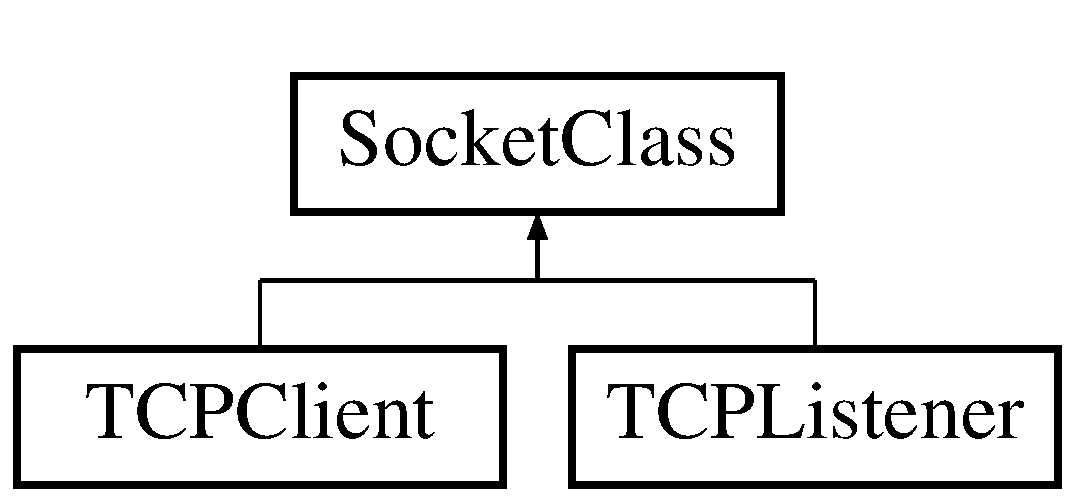
\includegraphics[height=2.000000cm]{classSocketClass}
\end{center}
\end{figure}
\subsection*{\-Public \-Member \-Functions}
\begin{DoxyCompactItemize}
\item 
\hyperlink{classSocketClass_a5ede881906dd99969280416e57713e6e}{\-Socket\-Class} ()
\item 
\hyperlink{classSocketClass_acb8c3d838def69ca9b596f4eeb082d65}{$\sim$\-Socket\-Class} ()
\item 
int \hyperlink{classSocketClass_ad628b8cf3503f4b3ff2f746f8f97222b}{close} ()
\item 
int \hyperlink{classSocketClass_a3cf341f54677aa0ebe3ffc51b663a2b1}{get\-Socket} ()
\item 
std\-::string \hyperlink{classSocketClass_a51c5674277badcbbd7d62fee52dc7cdb}{get\-Socket\-\_\-str} ()
\item 
void \hyperlink{classSocketClass_a12c2c67ee4907847be8d1067d8c211f5}{set\-Non\-Blocking} (int)
\end{DoxyCompactItemize}
\subsection*{\-Protected \-Member \-Functions}
\begin{DoxyCompactItemize}
\item 
int \hyperlink{classSocketClass_a1704e54e57a2aa6685148e37073fce6e}{tcp\-Socket} ()
\item 
int \hyperlink{classSocketClass_a27878d51b79e563cb8f7aa6a1d8c11d7}{tcp\-Socket} (int, int)
\end{DoxyCompactItemize}
\subsection*{\-Protected \-Attributes}
\begin{DoxyCompactItemize}
\item 
int \hyperlink{classSocketClass_a77c5d4d941abeb445665e2bce2fc48be}{socket\-Desc}
\item 
socklen\-\_\-t \hyperlink{classSocketClass_ab9712fd21de1ff87b027ddbbcf1ebd5a}{temp\-Len}
\item 
sockaddr \hyperlink{classSocketClass_a237dc3679dcac98a044b8eb31a6a3cf8}{temp\-Info}
\item 
sockaddr\-\_\-in \hyperlink{classSocketClass_a81f6c01eeabff07e468097f69c6efb9b}{info}
\end{DoxyCompactItemize}
\subsection*{\-Private \-Member \-Functions}
\begin{DoxyCompactItemize}
\item 
int \hyperlink{classSocketClass_aefba838dbd60b9f316b7c2d105212c7e}{new\-Socket} (int, int, int)
\end{DoxyCompactItemize}


\subsection{\-Constructor \& \-Destructor \-Documentation}
\hypertarget{classSocketClass_a5ede881906dd99969280416e57713e6e}{\index{\-Socket\-Class@{\-Socket\-Class}!\-Socket\-Class@{\-Socket\-Class}}
\index{\-Socket\-Class@{\-Socket\-Class}!SocketClass@{\-Socket\-Class}}
\subsubsection[{\-Socket\-Class}]{\setlength{\rightskip}{0pt plus 5cm}{\bf \-Socket\-Class\-::\-Socket\-Class} (
\begin{DoxyParamCaption}
{}
\end{DoxyParamCaption}
)}}\label{classSocketClass_a5ede881906dd99969280416e57713e6e}
\hypertarget{classSocketClass_acb8c3d838def69ca9b596f4eeb082d65}{\index{\-Socket\-Class@{\-Socket\-Class}!$\sim$\-Socket\-Class@{$\sim$\-Socket\-Class}}
\index{$\sim$\-Socket\-Class@{$\sim$\-Socket\-Class}!SocketClass@{\-Socket\-Class}}
\subsubsection[{$\sim$\-Socket\-Class}]{\setlength{\rightskip}{0pt plus 5cm}{\bf \-Socket\-Class\-::$\sim$\-Socket\-Class} (
\begin{DoxyParamCaption}
{}
\end{DoxyParamCaption}
)}}\label{classSocketClass_acb8c3d838def69ca9b596f4eeb082d65}


\subsection{\-Member \-Function \-Documentation}
\hypertarget{classSocketClass_ad628b8cf3503f4b3ff2f746f8f97222b}{\index{\-Socket\-Class@{\-Socket\-Class}!close@{close}}
\index{close@{close}!SocketClass@{\-Socket\-Class}}
\subsubsection[{close}]{\setlength{\rightskip}{0pt plus 5cm}int {\bf \-Socket\-Class\-::close} (
\begin{DoxyParamCaption}
{}
\end{DoxyParamCaption}
)}}\label{classSocketClass_ad628b8cf3503f4b3ff2f746f8f97222b}
\hypertarget{classSocketClass_a3cf341f54677aa0ebe3ffc51b663a2b1}{\index{\-Socket\-Class@{\-Socket\-Class}!get\-Socket@{get\-Socket}}
\index{get\-Socket@{get\-Socket}!SocketClass@{\-Socket\-Class}}
\subsubsection[{get\-Socket}]{\setlength{\rightskip}{0pt plus 5cm}int {\bf \-Socket\-Class\-::get\-Socket} (
\begin{DoxyParamCaption}
{}
\end{DoxyParamCaption}
)}}\label{classSocketClass_a3cf341f54677aa0ebe3ffc51b663a2b1}
\hypertarget{classSocketClass_a51c5674277badcbbd7d62fee52dc7cdb}{\index{\-Socket\-Class@{\-Socket\-Class}!get\-Socket\-\_\-str@{get\-Socket\-\_\-str}}
\index{get\-Socket\-\_\-str@{get\-Socket\-\_\-str}!SocketClass@{\-Socket\-Class}}
\subsubsection[{get\-Socket\-\_\-str}]{\setlength{\rightskip}{0pt plus 5cm}std\-::string {\bf \-Socket\-Class\-::get\-Socket\-\_\-str} (
\begin{DoxyParamCaption}
{}
\end{DoxyParamCaption}
)}}\label{classSocketClass_a51c5674277badcbbd7d62fee52dc7cdb}
\hypertarget{classSocketClass_aefba838dbd60b9f316b7c2d105212c7e}{\index{\-Socket\-Class@{\-Socket\-Class}!new\-Socket@{new\-Socket}}
\index{new\-Socket@{new\-Socket}!SocketClass@{\-Socket\-Class}}
\subsubsection[{new\-Socket}]{\setlength{\rightskip}{0pt plus 5cm}int {\bf \-Socket\-Class\-::new\-Socket} (
\begin{DoxyParamCaption}
\item[{int}]{socket\-\_\-family, }
\item[{int}]{socket\-\_\-type, }
\item[{int}]{protocol}
\end{DoxyParamCaption}
)\hspace{0.3cm}{\ttfamily  \mbox{[}private\mbox{]}}}}\label{classSocketClass_aefba838dbd60b9f316b7c2d105212c7e}
\hypertarget{classSocketClass_a12c2c67ee4907847be8d1067d8c211f5}{\index{\-Socket\-Class@{\-Socket\-Class}!set\-Non\-Blocking@{set\-Non\-Blocking}}
\index{set\-Non\-Blocking@{set\-Non\-Blocking}!SocketClass@{\-Socket\-Class}}
\subsubsection[{set\-Non\-Blocking}]{\setlength{\rightskip}{0pt plus 5cm}void {\bf \-Socket\-Class\-::set\-Non\-Blocking} (
\begin{DoxyParamCaption}
\item[{int}]{desc}
\end{DoxyParamCaption}
)}}\label{classSocketClass_a12c2c67ee4907847be8d1067d8c211f5}
\hypertarget{classSocketClass_a1704e54e57a2aa6685148e37073fce6e}{\index{\-Socket\-Class@{\-Socket\-Class}!tcp\-Socket@{tcp\-Socket}}
\index{tcp\-Socket@{tcp\-Socket}!SocketClass@{\-Socket\-Class}}
\subsubsection[{tcp\-Socket}]{\setlength{\rightskip}{0pt plus 5cm}int {\bf \-Socket\-Class\-::tcp\-Socket} (
\begin{DoxyParamCaption}
{}
\end{DoxyParamCaption}
)\hspace{0.3cm}{\ttfamily  \mbox{[}protected\mbox{]}}}}\label{classSocketClass_a1704e54e57a2aa6685148e37073fce6e}
\hypertarget{classSocketClass_a27878d51b79e563cb8f7aa6a1d8c11d7}{\index{\-Socket\-Class@{\-Socket\-Class}!tcp\-Socket@{tcp\-Socket}}
\index{tcp\-Socket@{tcp\-Socket}!SocketClass@{\-Socket\-Class}}
\subsubsection[{tcp\-Socket}]{\setlength{\rightskip}{0pt plus 5cm}int {\bf \-Socket\-Class\-::tcp\-Socket} (
\begin{DoxyParamCaption}
\item[{int}]{socket\-\_\-family, }
\item[{int}]{protocol}
\end{DoxyParamCaption}
)\hspace{0.3cm}{\ttfamily  \mbox{[}protected\mbox{]}}}}\label{classSocketClass_a27878d51b79e563cb8f7aa6a1d8c11d7}


\subsection{\-Field \-Documentation}
\hypertarget{classSocketClass_a81f6c01eeabff07e468097f69c6efb9b}{\index{\-Socket\-Class@{\-Socket\-Class}!info@{info}}
\index{info@{info}!SocketClass@{\-Socket\-Class}}
\subsubsection[{info}]{\setlength{\rightskip}{0pt plus 5cm}sockaddr\-\_\-in {\bf \-Socket\-Class\-::info}\hspace{0.3cm}{\ttfamily  \mbox{[}protected\mbox{]}}}}\label{classSocketClass_a81f6c01eeabff07e468097f69c6efb9b}
\hypertarget{classSocketClass_a77c5d4d941abeb445665e2bce2fc48be}{\index{\-Socket\-Class@{\-Socket\-Class}!socket\-Desc@{socket\-Desc}}
\index{socket\-Desc@{socket\-Desc}!SocketClass@{\-Socket\-Class}}
\subsubsection[{socket\-Desc}]{\setlength{\rightskip}{0pt plus 5cm}int {\bf \-Socket\-Class\-::socket\-Desc}\hspace{0.3cm}{\ttfamily  \mbox{[}protected\mbox{]}}}}\label{classSocketClass_a77c5d4d941abeb445665e2bce2fc48be}
\hypertarget{classSocketClass_a237dc3679dcac98a044b8eb31a6a3cf8}{\index{\-Socket\-Class@{\-Socket\-Class}!temp\-Info@{temp\-Info}}
\index{temp\-Info@{temp\-Info}!SocketClass@{\-Socket\-Class}}
\subsubsection[{temp\-Info}]{\setlength{\rightskip}{0pt plus 5cm}sockaddr {\bf \-Socket\-Class\-::temp\-Info}\hspace{0.3cm}{\ttfamily  \mbox{[}protected\mbox{]}}}}\label{classSocketClass_a237dc3679dcac98a044b8eb31a6a3cf8}
\hypertarget{classSocketClass_ab9712fd21de1ff87b027ddbbcf1ebd5a}{\index{\-Socket\-Class@{\-Socket\-Class}!temp\-Len@{temp\-Len}}
\index{temp\-Len@{temp\-Len}!SocketClass@{\-Socket\-Class}}
\subsubsection[{temp\-Len}]{\setlength{\rightskip}{0pt plus 5cm}socklen\-\_\-t {\bf \-Socket\-Class\-::temp\-Len}\hspace{0.3cm}{\ttfamily  \mbox{[}protected\mbox{]}}}}\label{classSocketClass_ab9712fd21de1ff87b027ddbbcf1ebd5a}


\-The documentation for this class was generated from the following files\-:\begin{DoxyCompactItemize}
\item 
common/\hyperlink{SocketClass_8h}{\-Socket\-Class.\-h}\item 
common/\hyperlink{SocketClass_8cpp}{\-Socket\-Class.\-cpp}\end{DoxyCompactItemize}

\hypertarget{classSQLite}{\section{\-S\-Q\-Lite \-Class \-Reference}
\label{classSQLite}\index{\-S\-Q\-Lite@{\-S\-Q\-Lite}}
}


{\ttfamily \#include $<$\-S\-Q\-Lite.\-h$>$}

\subsection*{\-Public \-Member \-Functions}
\begin{DoxyCompactItemize}
\item 
\hyperlink{classSQLite_ae7b35dc7e3c41543a0acde669ad4ba0d}{\-S\-Q\-Lite} ()
\item 
\hyperlink{classSQLite_a5b30b82149fe1cc07046f25a9935747f}{$\sim$\-S\-Q\-Lite} ()
\item 
void \hyperlink{classSQLite_a1937c8a95aebbfc9b82bf7b30aa6375d}{log} (std\-::string)
\item 
bool \hyperlink{classSQLite_a421fe9dd5fd1abd92b00857253823c90}{connect} (std\-::string)
\item 
void \hyperlink{classSQLite_af4a886ee189358e84337a5e81ed0d515}{disconnect} ()
\item 
int \hyperlink{classSQLite_a4124efb4d6521bcad1666d949ae36311}{query} (std\-::string)
\item 
int \hyperlink{classSQLite_addf9309356a45a01f74831cb803b4b8d}{update} (std\-::string)
\item 
int \hyperlink{classSQLite_a985917c1b24cfdc802851d22f5d17c3e}{has\-Next} ()
\item 
std\-::vector$<$ std\-::string $>$ \hyperlink{classSQLite_ad85ca830bc58aa3c299489c2eaa90080}{next} ()
\end{DoxyCompactItemize}
\subsection*{\-Private \-Attributes}
\begin{DoxyCompactItemize}
\item 
int \hyperlink{classSQLite_add18111d5de9e218a147dbceb0aa7899}{has\-Next\-Row}
\item 
sqlite3\-\_\-stmt $\ast$ \hyperlink{classSQLite_ac9fcbb5e55073780e5b7a6b10147d74e}{statement}
\item 
sqlite3 $\ast$ \hyperlink{classSQLite_a206e8b4696cbea9d8091310cf17213ee}{dbfile}
\item 
bool \hyperlink{classSQLite_a7d855ec7c6e9644201b59321375a6fa5}{is\-Open\-D\-B}
\end{DoxyCompactItemize}


\subsection{\-Constructor \& \-Destructor \-Documentation}
\hypertarget{classSQLite_ae7b35dc7e3c41543a0acde669ad4ba0d}{\index{\-S\-Q\-Lite@{\-S\-Q\-Lite}!\-S\-Q\-Lite@{\-S\-Q\-Lite}}
\index{\-S\-Q\-Lite@{\-S\-Q\-Lite}!SQLite@{\-S\-Q\-Lite}}
\subsubsection[{\-S\-Q\-Lite}]{\setlength{\rightskip}{0pt plus 5cm}{\bf \-S\-Q\-Lite\-::\-S\-Q\-Lite} (
\begin{DoxyParamCaption}
{}
\end{DoxyParamCaption}
)}}\label{classSQLite_ae7b35dc7e3c41543a0acde669ad4ba0d}
\hypertarget{classSQLite_a5b30b82149fe1cc07046f25a9935747f}{\index{\-S\-Q\-Lite@{\-S\-Q\-Lite}!$\sim$\-S\-Q\-Lite@{$\sim$\-S\-Q\-Lite}}
\index{$\sim$\-S\-Q\-Lite@{$\sim$\-S\-Q\-Lite}!SQLite@{\-S\-Q\-Lite}}
\subsubsection[{$\sim$\-S\-Q\-Lite}]{\setlength{\rightskip}{0pt plus 5cm}{\bf \-S\-Q\-Lite\-::$\sim$\-S\-Q\-Lite} (
\begin{DoxyParamCaption}
{}
\end{DoxyParamCaption}
)}}\label{classSQLite_a5b30b82149fe1cc07046f25a9935747f}


\subsection{\-Member \-Function \-Documentation}
\hypertarget{classSQLite_a421fe9dd5fd1abd92b00857253823c90}{\index{\-S\-Q\-Lite@{\-S\-Q\-Lite}!connect@{connect}}
\index{connect@{connect}!SQLite@{\-S\-Q\-Lite}}
\subsubsection[{connect}]{\setlength{\rightskip}{0pt plus 5cm}bool {\bf \-S\-Q\-Lite\-::connect} (
\begin{DoxyParamCaption}
\item[{std\-::string}]{db}
\end{DoxyParamCaption}
)}}\label{classSQLite_a421fe9dd5fd1abd92b00857253823c90}
\hypertarget{classSQLite_af4a886ee189358e84337a5e81ed0d515}{\index{\-S\-Q\-Lite@{\-S\-Q\-Lite}!disconnect@{disconnect}}
\index{disconnect@{disconnect}!SQLite@{\-S\-Q\-Lite}}
\subsubsection[{disconnect}]{\setlength{\rightskip}{0pt plus 5cm}void {\bf \-S\-Q\-Lite\-::disconnect} (
\begin{DoxyParamCaption}
{}
\end{DoxyParamCaption}
)}}\label{classSQLite_af4a886ee189358e84337a5e81ed0d515}
\hypertarget{classSQLite_a985917c1b24cfdc802851d22f5d17c3e}{\index{\-S\-Q\-Lite@{\-S\-Q\-Lite}!has\-Next@{has\-Next}}
\index{has\-Next@{has\-Next}!SQLite@{\-S\-Q\-Lite}}
\subsubsection[{has\-Next}]{\setlength{\rightskip}{0pt plus 5cm}int {\bf \-S\-Q\-Lite\-::has\-Next} (
\begin{DoxyParamCaption}
{}
\end{DoxyParamCaption}
)}}\label{classSQLite_a985917c1b24cfdc802851d22f5d17c3e}
\hypertarget{classSQLite_a1937c8a95aebbfc9b82bf7b30aa6375d}{\index{\-S\-Q\-Lite@{\-S\-Q\-Lite}!log@{log}}
\index{log@{log}!SQLite@{\-S\-Q\-Lite}}
\subsubsection[{log}]{\setlength{\rightskip}{0pt plus 5cm}void {\bf \-S\-Q\-Lite\-::log} (
\begin{DoxyParamCaption}
\item[{std\-::string}]{msg}
\end{DoxyParamCaption}
)}}\label{classSQLite_a1937c8a95aebbfc9b82bf7b30aa6375d}
\hypertarget{classSQLite_ad85ca830bc58aa3c299489c2eaa90080}{\index{\-S\-Q\-Lite@{\-S\-Q\-Lite}!next@{next}}
\index{next@{next}!SQLite@{\-S\-Q\-Lite}}
\subsubsection[{next}]{\setlength{\rightskip}{0pt plus 5cm}std\-::vector$<$ std\-::string $>$ {\bf \-S\-Q\-Lite\-::next} (
\begin{DoxyParamCaption}
{}
\end{DoxyParamCaption}
)}}\label{classSQLite_ad85ca830bc58aa3c299489c2eaa90080}
\hypertarget{classSQLite_a4124efb4d6521bcad1666d949ae36311}{\index{\-S\-Q\-Lite@{\-S\-Q\-Lite}!query@{query}}
\index{query@{query}!SQLite@{\-S\-Q\-Lite}}
\subsubsection[{query}]{\setlength{\rightskip}{0pt plus 5cm}int {\bf \-S\-Q\-Lite\-::query} (
\begin{DoxyParamCaption}
\item[{std\-::string}]{q}
\end{DoxyParamCaption}
)}}\label{classSQLite_a4124efb4d6521bcad1666d949ae36311}
\hypertarget{classSQLite_addf9309356a45a01f74831cb803b4b8d}{\index{\-S\-Q\-Lite@{\-S\-Q\-Lite}!update@{update}}
\index{update@{update}!SQLite@{\-S\-Q\-Lite}}
\subsubsection[{update}]{\setlength{\rightskip}{0pt plus 5cm}int {\bf \-S\-Q\-Lite\-::update} (
\begin{DoxyParamCaption}
\item[{std\-::string}]{q}
\end{DoxyParamCaption}
)}}\label{classSQLite_addf9309356a45a01f74831cb803b4b8d}


\subsection{\-Field \-Documentation}
\hypertarget{classSQLite_a206e8b4696cbea9d8091310cf17213ee}{\index{\-S\-Q\-Lite@{\-S\-Q\-Lite}!dbfile@{dbfile}}
\index{dbfile@{dbfile}!SQLite@{\-S\-Q\-Lite}}
\subsubsection[{dbfile}]{\setlength{\rightskip}{0pt plus 5cm}sqlite3$\ast$ {\bf \-S\-Q\-Lite\-::dbfile}\hspace{0.3cm}{\ttfamily  \mbox{[}private\mbox{]}}}}\label{classSQLite_a206e8b4696cbea9d8091310cf17213ee}
\hypertarget{classSQLite_add18111d5de9e218a147dbceb0aa7899}{\index{\-S\-Q\-Lite@{\-S\-Q\-Lite}!has\-Next\-Row@{has\-Next\-Row}}
\index{has\-Next\-Row@{has\-Next\-Row}!SQLite@{\-S\-Q\-Lite}}
\subsubsection[{has\-Next\-Row}]{\setlength{\rightskip}{0pt plus 5cm}int {\bf \-S\-Q\-Lite\-::has\-Next\-Row}\hspace{0.3cm}{\ttfamily  \mbox{[}private\mbox{]}}}}\label{classSQLite_add18111d5de9e218a147dbceb0aa7899}
\hypertarget{classSQLite_a7d855ec7c6e9644201b59321375a6fa5}{\index{\-S\-Q\-Lite@{\-S\-Q\-Lite}!is\-Open\-D\-B@{is\-Open\-D\-B}}
\index{is\-Open\-D\-B@{is\-Open\-D\-B}!SQLite@{\-S\-Q\-Lite}}
\subsubsection[{is\-Open\-D\-B}]{\setlength{\rightskip}{0pt plus 5cm}bool {\bf \-S\-Q\-Lite\-::is\-Open\-D\-B}\hspace{0.3cm}{\ttfamily  \mbox{[}private\mbox{]}}}}\label{classSQLite_a7d855ec7c6e9644201b59321375a6fa5}
\hypertarget{classSQLite_ac9fcbb5e55073780e5b7a6b10147d74e}{\index{\-S\-Q\-Lite@{\-S\-Q\-Lite}!statement@{statement}}
\index{statement@{statement}!SQLite@{\-S\-Q\-Lite}}
\subsubsection[{statement}]{\setlength{\rightskip}{0pt plus 5cm}sqlite3\-\_\-stmt$\ast$ {\bf \-S\-Q\-Lite\-::statement}\hspace{0.3cm}{\ttfamily  \mbox{[}private\mbox{]}}}}\label{classSQLite_ac9fcbb5e55073780e5b7a6b10147d74e}


\-The documentation for this class was generated from the following files\-:\begin{DoxyCompactItemize}
\item 
sqlite/\hyperlink{SQLite_8h}{\-S\-Q\-Lite.\-h}\item 
sqlite/\hyperlink{SQLite_8cpp}{\-S\-Q\-Lite.\-cpp}\end{DoxyCompactItemize}

\hypertarget{classTCPClient}{\section{\-T\-C\-P\-Client \-Class \-Reference}
\label{classTCPClient}\index{\-T\-C\-P\-Client@{\-T\-C\-P\-Client}}
}


{\ttfamily \#include $<$\-T\-C\-P\-Client.\-h$>$}

\-Inheritance diagram for \-T\-C\-P\-Client\-:\begin{figure}[H]
\begin{center}
\leavevmode
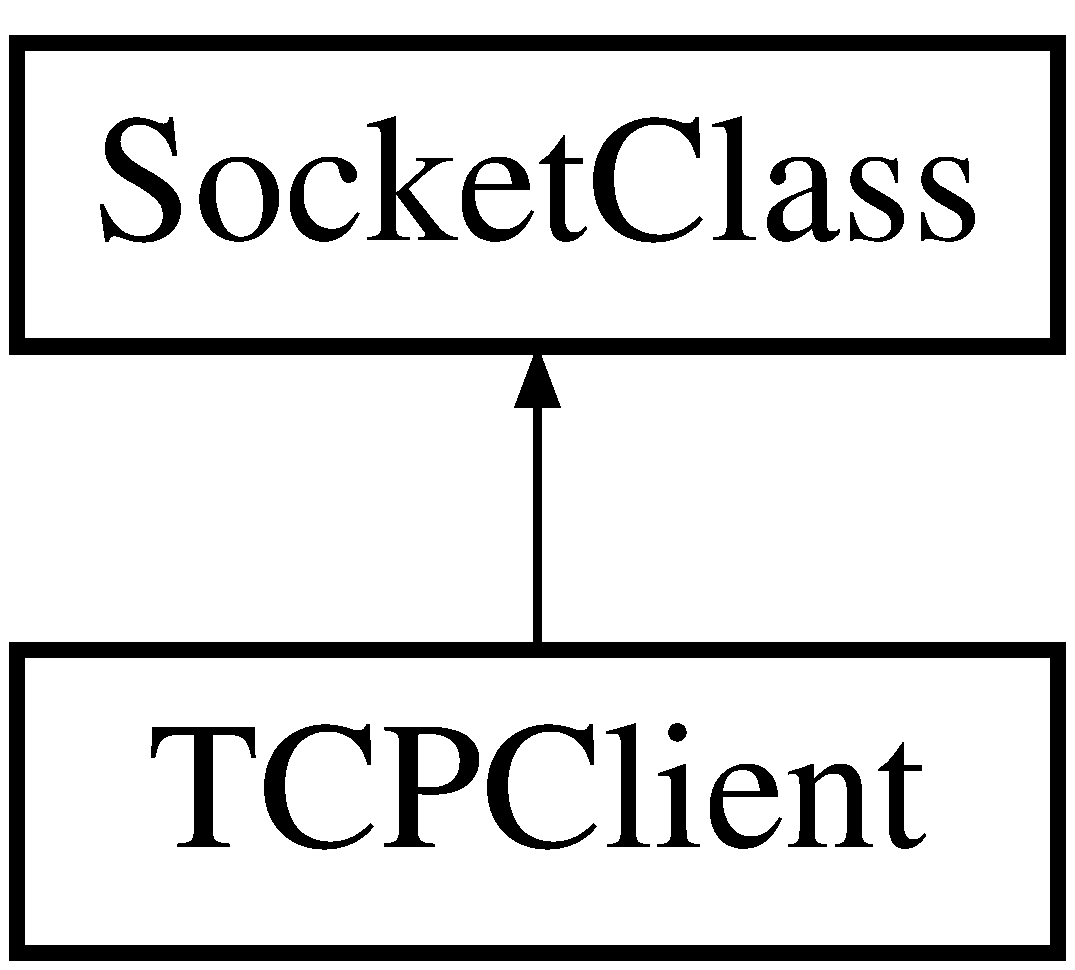
\includegraphics[height=2.000000cm]{classTCPClient}
\end{center}
\end{figure}
\subsection*{\-Public \-Member \-Functions}
\begin{DoxyCompactItemize}
\item 
\hyperlink{classTCPClient_ad37bba4f2ebcc899b9871656802dcbe9}{\-T\-C\-P\-Client} ()
\item 
\hyperlink{classTCPClient_aa348b6919298978537c7921ee185ffd6}{\-T\-C\-P\-Client} (int)
\item 
\hyperlink{classTCPClient_a869a5b3319ca562d03cb4c59ebec4407}{$\sim$\-T\-C\-P\-Client} ()
\item 
int \hyperlink{classTCPClient_a1629ed9ba8cd5a29daefc530cad68ebf}{connect} (const char $\ast$, const char $\ast$)
\item 
int \hyperlink{classTCPClient_abbccd38e761fb550749504dbe26c8cdf}{recv} (void $\ast$, size\-\_\-t len)
\item 
int \hyperlink{classTCPClient_ab89b479cb995571d860587e43333730c}{send} (const void $\ast$, size\-\_\-t len)
\item 
void $\ast$ \hyperlink{classTCPClient_a63fdb0cbcc66300ffe84445b30c626f1}{get\-\_\-in\-\_\-addr} (struct sockaddr $\ast$)
\end{DoxyCompactItemize}
\subsection*{\-Private \-Attributes}
\begin{DoxyCompactItemize}
\item 
bool \hyperlink{classTCPClient_a1d653a3fc1b8c2235eac2997d35bbf53}{is\-Connected}
\end{DoxyCompactItemize}


\subsection{\-Constructor \& \-Destructor \-Documentation}
\hypertarget{classTCPClient_ad37bba4f2ebcc899b9871656802dcbe9}{\index{\-T\-C\-P\-Client@{\-T\-C\-P\-Client}!\-T\-C\-P\-Client@{\-T\-C\-P\-Client}}
\index{\-T\-C\-P\-Client@{\-T\-C\-P\-Client}!TCPClient@{\-T\-C\-P\-Client}}
\subsubsection[{\-T\-C\-P\-Client}]{\setlength{\rightskip}{0pt plus 5cm}{\bf \-T\-C\-P\-Client\-::\-T\-C\-P\-Client} (
\begin{DoxyParamCaption}
{}
\end{DoxyParamCaption}
)}}\label{classTCPClient_ad37bba4f2ebcc899b9871656802dcbe9}
\hypertarget{classTCPClient_aa348b6919298978537c7921ee185ffd6}{\index{\-T\-C\-P\-Client@{\-T\-C\-P\-Client}!\-T\-C\-P\-Client@{\-T\-C\-P\-Client}}
\index{\-T\-C\-P\-Client@{\-T\-C\-P\-Client}!TCPClient@{\-T\-C\-P\-Client}}
\subsubsection[{\-T\-C\-P\-Client}]{\setlength{\rightskip}{0pt plus 5cm}{\bf \-T\-C\-P\-Client\-::\-T\-C\-P\-Client} (
\begin{DoxyParamCaption}
\item[{int}]{desc}
\end{DoxyParamCaption}
)}}\label{classTCPClient_aa348b6919298978537c7921ee185ffd6}
\hypertarget{classTCPClient_a869a5b3319ca562d03cb4c59ebec4407}{\index{\-T\-C\-P\-Client@{\-T\-C\-P\-Client}!$\sim$\-T\-C\-P\-Client@{$\sim$\-T\-C\-P\-Client}}
\index{$\sim$\-T\-C\-P\-Client@{$\sim$\-T\-C\-P\-Client}!TCPClient@{\-T\-C\-P\-Client}}
\subsubsection[{$\sim$\-T\-C\-P\-Client}]{\setlength{\rightskip}{0pt plus 5cm}{\bf \-T\-C\-P\-Client\-::$\sim$\-T\-C\-P\-Client} (
\begin{DoxyParamCaption}
{}
\end{DoxyParamCaption}
)}}\label{classTCPClient_a869a5b3319ca562d03cb4c59ebec4407}


\subsection{\-Member \-Function \-Documentation}
\hypertarget{classTCPClient_a1629ed9ba8cd5a29daefc530cad68ebf}{\index{\-T\-C\-P\-Client@{\-T\-C\-P\-Client}!connect@{connect}}
\index{connect@{connect}!TCPClient@{\-T\-C\-P\-Client}}
\subsubsection[{connect}]{\setlength{\rightskip}{0pt plus 5cm}int {\bf \-T\-C\-P\-Client\-::connect} (
\begin{DoxyParamCaption}
\item[{const char $\ast$}]{ip, }
\item[{const char $\ast$}]{port}
\end{DoxyParamCaption}
)}}\label{classTCPClient_a1629ed9ba8cd5a29daefc530cad68ebf}
\hypertarget{classTCPClient_a63fdb0cbcc66300ffe84445b30c626f1}{\index{\-T\-C\-P\-Client@{\-T\-C\-P\-Client}!get\-\_\-in\-\_\-addr@{get\-\_\-in\-\_\-addr}}
\index{get\-\_\-in\-\_\-addr@{get\-\_\-in\-\_\-addr}!TCPClient@{\-T\-C\-P\-Client}}
\subsubsection[{get\-\_\-in\-\_\-addr}]{\setlength{\rightskip}{0pt plus 5cm}void $\ast$ {\bf \-T\-C\-P\-Client\-::get\-\_\-in\-\_\-addr} (
\begin{DoxyParamCaption}
\item[{struct sockaddr $\ast$}]{sa}
\end{DoxyParamCaption}
)}}\label{classTCPClient_a63fdb0cbcc66300ffe84445b30c626f1}
\hypertarget{classTCPClient_abbccd38e761fb550749504dbe26c8cdf}{\index{\-T\-C\-P\-Client@{\-T\-C\-P\-Client}!recv@{recv}}
\index{recv@{recv}!TCPClient@{\-T\-C\-P\-Client}}
\subsubsection[{recv}]{\setlength{\rightskip}{0pt plus 5cm}int {\bf \-T\-C\-P\-Client\-::recv} (
\begin{DoxyParamCaption}
\item[{void $\ast$}]{buffer, }
\item[{size\-\_\-t}]{len}
\end{DoxyParamCaption}
)}}\label{classTCPClient_abbccd38e761fb550749504dbe26c8cdf}
\hypertarget{classTCPClient_ab89b479cb995571d860587e43333730c}{\index{\-T\-C\-P\-Client@{\-T\-C\-P\-Client}!send@{send}}
\index{send@{send}!TCPClient@{\-T\-C\-P\-Client}}
\subsubsection[{send}]{\setlength{\rightskip}{0pt plus 5cm}int {\bf \-T\-C\-P\-Client\-::send} (
\begin{DoxyParamCaption}
\item[{const void $\ast$}]{buffer, }
\item[{size\-\_\-t}]{len}
\end{DoxyParamCaption}
)}}\label{classTCPClient_ab89b479cb995571d860587e43333730c}


\subsection{\-Field \-Documentation}
\hypertarget{classTCPClient_a1d653a3fc1b8c2235eac2997d35bbf53}{\index{\-T\-C\-P\-Client@{\-T\-C\-P\-Client}!is\-Connected@{is\-Connected}}
\index{is\-Connected@{is\-Connected}!TCPClient@{\-T\-C\-P\-Client}}
\subsubsection[{is\-Connected}]{\setlength{\rightskip}{0pt plus 5cm}bool {\bf \-T\-C\-P\-Client\-::is\-Connected}\hspace{0.3cm}{\ttfamily  \mbox{[}private\mbox{]}}}}\label{classTCPClient_a1d653a3fc1b8c2235eac2997d35bbf53}


\-The documentation for this class was generated from the following files\-:\begin{DoxyCompactItemize}
\item 
common/\hyperlink{TCPClient_8h}{\-T\-C\-P\-Client.\-h}\item 
common/\hyperlink{TCPClient_8cpp}{\-T\-C\-P\-Client.\-cpp}\end{DoxyCompactItemize}

\hypertarget{classTCPListener}{\section{\-T\-C\-P\-Listener \-Class \-Reference}
\label{classTCPListener}\index{\-T\-C\-P\-Listener@{\-T\-C\-P\-Listener}}
}


{\ttfamily \#include $<$\-T\-C\-P\-Listener.\-h$>$}

\-Inheritance diagram for \-T\-C\-P\-Listener\-:\begin{figure}[H]
\begin{center}
\leavevmode
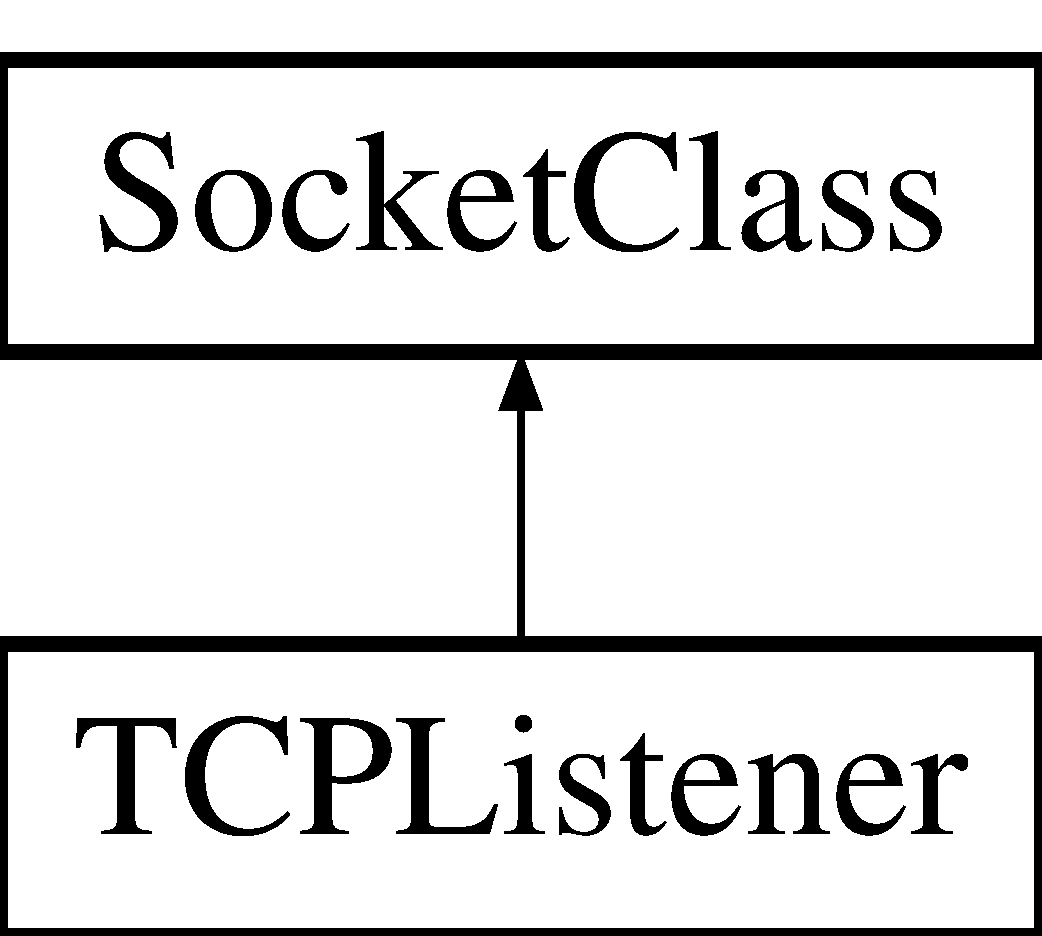
\includegraphics[height=2.000000cm]{classTCPListener}
\end{center}
\end{figure}
\subsection*{\-Public \-Member \-Functions}
\begin{DoxyCompactItemize}
\item 
\hyperlink{classTCPListener_a58f2fc8c4992d63691cff12519279758}{\-T\-C\-P\-Listener} ()
\item 
\hyperlink{classTCPListener_af7e560c0c6c0ea486113dc6eabc4226d}{$\sim$\-T\-C\-P\-Listener} ()
\item 
void \hyperlink{classTCPListener_ab207b5227e906dd9a956cfd0243349b2}{reset\-Port} (int)
\item 
bool \hyperlink{classTCPListener_ae0b28ea37c99b35ae76e7eaee05aba87}{bind} (int)
\item 
bool \hyperlink{classTCPListener_a0dc5951a6f84afa2991d06b97114ba0e}{listen} (int)
\item 
int \hyperlink{classTCPListener_ab640f1bbae40d42f8838d64b7ac90e52}{accept} ()
\end{DoxyCompactItemize}
\subsection*{\-Private \-Attributes}
\begin{DoxyCompactItemize}
\item 
int \hyperlink{classTCPListener_adb28c377cc7edd8011e2171027ad163e}{port\-Number}
\item 
int \hyperlink{classTCPListener_ad8dcabf3ed2e479f8c518a5b31a9b143}{queue\-List}
\item 
bool \hyperlink{classTCPListener_ae2a201690fd3e302cf2a04be52617b48}{is\-Binded}
\item 
bool \hyperlink{classTCPListener_ab7f4c0050982e82238e463186abd683b}{is\-Listening}
\end{DoxyCompactItemize}


\subsection{\-Constructor \& \-Destructor \-Documentation}
\hypertarget{classTCPListener_a58f2fc8c4992d63691cff12519279758}{\index{\-T\-C\-P\-Listener@{\-T\-C\-P\-Listener}!\-T\-C\-P\-Listener@{\-T\-C\-P\-Listener}}
\index{\-T\-C\-P\-Listener@{\-T\-C\-P\-Listener}!TCPListener@{\-T\-C\-P\-Listener}}
\subsubsection[{\-T\-C\-P\-Listener}]{\setlength{\rightskip}{0pt plus 5cm}{\bf \-T\-C\-P\-Listener\-::\-T\-C\-P\-Listener} (
\begin{DoxyParamCaption}
{}
\end{DoxyParamCaption}
)}}\label{classTCPListener_a58f2fc8c4992d63691cff12519279758}
\hypertarget{classTCPListener_af7e560c0c6c0ea486113dc6eabc4226d}{\index{\-T\-C\-P\-Listener@{\-T\-C\-P\-Listener}!$\sim$\-T\-C\-P\-Listener@{$\sim$\-T\-C\-P\-Listener}}
\index{$\sim$\-T\-C\-P\-Listener@{$\sim$\-T\-C\-P\-Listener}!TCPListener@{\-T\-C\-P\-Listener}}
\subsubsection[{$\sim$\-T\-C\-P\-Listener}]{\setlength{\rightskip}{0pt plus 5cm}{\bf \-T\-C\-P\-Listener\-::$\sim$\-T\-C\-P\-Listener} (
\begin{DoxyParamCaption}
{}
\end{DoxyParamCaption}
)}}\label{classTCPListener_af7e560c0c6c0ea486113dc6eabc4226d}


\subsection{\-Member \-Function \-Documentation}
\hypertarget{classTCPListener_ab640f1bbae40d42f8838d64b7ac90e52}{\index{\-T\-C\-P\-Listener@{\-T\-C\-P\-Listener}!accept@{accept}}
\index{accept@{accept}!TCPListener@{\-T\-C\-P\-Listener}}
\subsubsection[{accept}]{\setlength{\rightskip}{0pt plus 5cm}int {\bf \-T\-C\-P\-Listener\-::accept} (
\begin{DoxyParamCaption}
{}
\end{DoxyParamCaption}
)}}\label{classTCPListener_ab640f1bbae40d42f8838d64b7ac90e52}
\hypertarget{classTCPListener_ae0b28ea37c99b35ae76e7eaee05aba87}{\index{\-T\-C\-P\-Listener@{\-T\-C\-P\-Listener}!bind@{bind}}
\index{bind@{bind}!TCPListener@{\-T\-C\-P\-Listener}}
\subsubsection[{bind}]{\setlength{\rightskip}{0pt plus 5cm}bool {\bf \-T\-C\-P\-Listener\-::bind} (
\begin{DoxyParamCaption}
\item[{int}]{port}
\end{DoxyParamCaption}
)}}\label{classTCPListener_ae0b28ea37c99b35ae76e7eaee05aba87}
\hypertarget{classTCPListener_a0dc5951a6f84afa2991d06b97114ba0e}{\index{\-T\-C\-P\-Listener@{\-T\-C\-P\-Listener}!listen@{listen}}
\index{listen@{listen}!TCPListener@{\-T\-C\-P\-Listener}}
\subsubsection[{listen}]{\setlength{\rightskip}{0pt plus 5cm}bool {\bf \-T\-C\-P\-Listener\-::listen} (
\begin{DoxyParamCaption}
\item[{int}]{queue}
\end{DoxyParamCaption}
)}}\label{classTCPListener_a0dc5951a6f84afa2991d06b97114ba0e}
\hypertarget{classTCPListener_ab207b5227e906dd9a956cfd0243349b2}{\index{\-T\-C\-P\-Listener@{\-T\-C\-P\-Listener}!reset\-Port@{reset\-Port}}
\index{reset\-Port@{reset\-Port}!TCPListener@{\-T\-C\-P\-Listener}}
\subsubsection[{reset\-Port}]{\setlength{\rightskip}{0pt plus 5cm}void {\bf \-T\-C\-P\-Listener\-::reset\-Port} (
\begin{DoxyParamCaption}
\item[{int}]{desc}
\end{DoxyParamCaption}
)}}\label{classTCPListener_ab207b5227e906dd9a956cfd0243349b2}


\subsection{\-Field \-Documentation}
\hypertarget{classTCPListener_ae2a201690fd3e302cf2a04be52617b48}{\index{\-T\-C\-P\-Listener@{\-T\-C\-P\-Listener}!is\-Binded@{is\-Binded}}
\index{is\-Binded@{is\-Binded}!TCPListener@{\-T\-C\-P\-Listener}}
\subsubsection[{is\-Binded}]{\setlength{\rightskip}{0pt plus 5cm}bool {\bf \-T\-C\-P\-Listener\-::is\-Binded}\hspace{0.3cm}{\ttfamily  \mbox{[}private\mbox{]}}}}\label{classTCPListener_ae2a201690fd3e302cf2a04be52617b48}
\hypertarget{classTCPListener_ab7f4c0050982e82238e463186abd683b}{\index{\-T\-C\-P\-Listener@{\-T\-C\-P\-Listener}!is\-Listening@{is\-Listening}}
\index{is\-Listening@{is\-Listening}!TCPListener@{\-T\-C\-P\-Listener}}
\subsubsection[{is\-Listening}]{\setlength{\rightskip}{0pt plus 5cm}bool {\bf \-T\-C\-P\-Listener\-::is\-Listening}\hspace{0.3cm}{\ttfamily  \mbox{[}private\mbox{]}}}}\label{classTCPListener_ab7f4c0050982e82238e463186abd683b}
\hypertarget{classTCPListener_adb28c377cc7edd8011e2171027ad163e}{\index{\-T\-C\-P\-Listener@{\-T\-C\-P\-Listener}!port\-Number@{port\-Number}}
\index{port\-Number@{port\-Number}!TCPListener@{\-T\-C\-P\-Listener}}
\subsubsection[{port\-Number}]{\setlength{\rightskip}{0pt plus 5cm}int {\bf \-T\-C\-P\-Listener\-::port\-Number}\hspace{0.3cm}{\ttfamily  \mbox{[}private\mbox{]}}}}\label{classTCPListener_adb28c377cc7edd8011e2171027ad163e}
\hypertarget{classTCPListener_ad8dcabf3ed2e479f8c518a5b31a9b143}{\index{\-T\-C\-P\-Listener@{\-T\-C\-P\-Listener}!queue\-List@{queue\-List}}
\index{queue\-List@{queue\-List}!TCPListener@{\-T\-C\-P\-Listener}}
\subsubsection[{queue\-List}]{\setlength{\rightskip}{0pt plus 5cm}int {\bf \-T\-C\-P\-Listener\-::queue\-List}\hspace{0.3cm}{\ttfamily  \mbox{[}private\mbox{]}}}}\label{classTCPListener_ad8dcabf3ed2e479f8c518a5b31a9b143}


\-The documentation for this class was generated from the following files\-:\begin{DoxyCompactItemize}
\item 
common/\hyperlink{TCPListener_8h}{\-T\-C\-P\-Listener.\-h}\item 
common/\hyperlink{TCPListener_8cpp}{\-T\-C\-P\-Listener.\-cpp}\end{DoxyCompactItemize}

\hypertarget{classThreadClass}{\section{\-Thread\-Class \-Class \-Reference}
\label{classThreadClass}\index{\-Thread\-Class@{\-Thread\-Class}}
}


{\ttfamily \#include $<$\-Thread\-Class.\-h$>$}

\-Inheritance diagram for \-Thread\-Class\-:\begin{figure}[H]
\begin{center}
\leavevmode
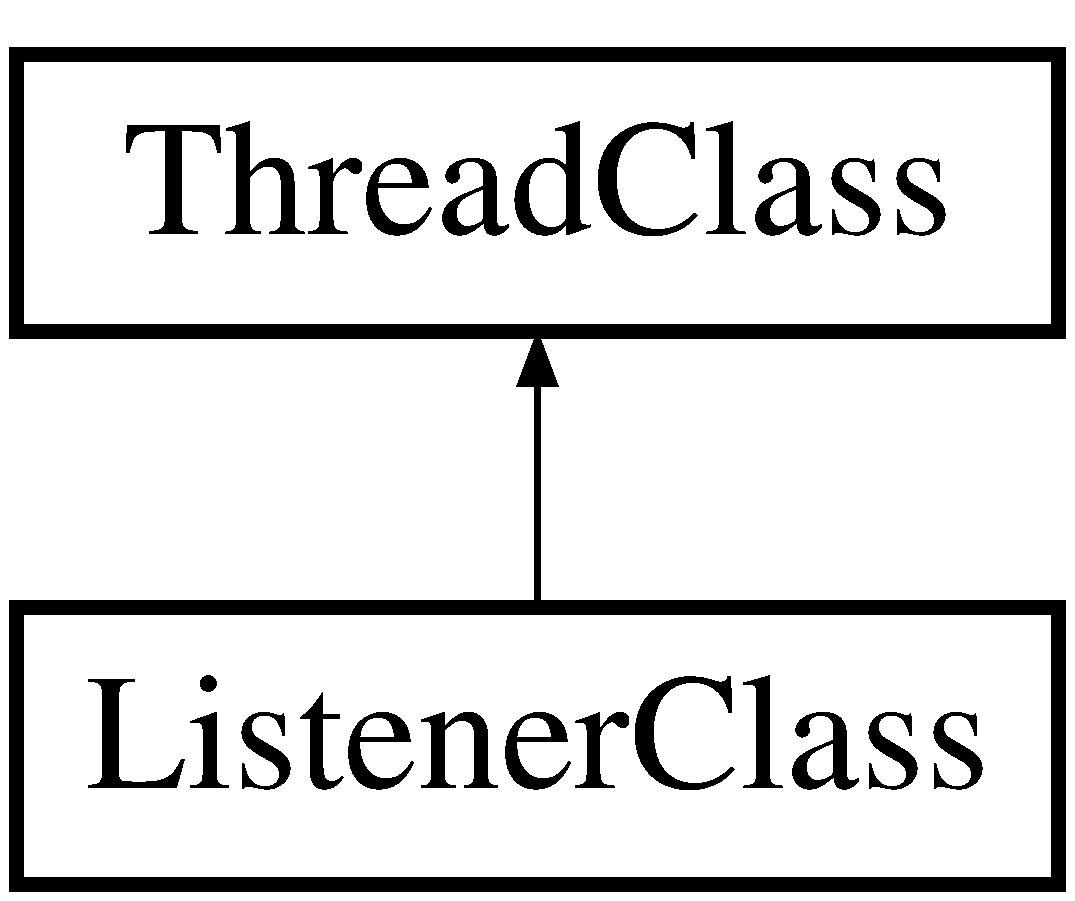
\includegraphics[height=2.000000cm]{classThreadClass}
\end{center}
\end{figure}
\subsection*{\-Public \-Member \-Functions}
\begin{DoxyCompactItemize}
\item 
\hyperlink{classThreadClass_ac19d9b2f09e438d5068342bd02ff5661}{\-Thread\-Class} ()
\item 
\hyperlink{classThreadClass_a61dc219271efbbb059e5d78fd2a4e0ac}{$\sim$\-Thread\-Class} ()
\item 
int \hyperlink{classThreadClass_a6e0e65009911bab842025725b87a48a0}{\-Start} (void $\ast$arg)
\item 
void \hyperlink{classThreadClass_a199c95085d110a47c5a83da0529d90f2}{\-Wait} ()
\end{DoxyCompactItemize}
\subsection*{\-Protected \-Member \-Functions}
\begin{DoxyCompactItemize}
\item 
void $\ast$ \hyperlink{classThreadClass_a06fd94929154dbcb74adfb5fe4c430d3}{get\-Arg} ()
\item 
void \hyperlink{classThreadClass_ac5077b7e70c5634bd82e2739f9d486bd}{set\-Arg} (void $\ast$arg)
\item 
void \hyperlink{classThreadClass_af8d3455f41b943c445c4894fbec9a9a7}{set\-Status} (bool)
\item 
void \hyperlink{classThreadClass_aa3a152dd553c2dd4326eeafc13b3e562}{wake} ()
\item 
int \hyperlink{classThreadClass_ab9fc65d8931c6de24bb8d7659397a491}{\-Run} ()
\item 
bool \hyperlink{classThreadClass_a039630a7228034cd111fe5d461a5e9fe}{get\-Status} ()
\item 
virtual void \hyperlink{classThreadClass_a79775d1799a12bf4c9575cad8fd462d0}{\-Setup} ()=0
\item 
virtual void \hyperlink{classThreadClass_aa6b3fb3567bd8b7d67b4aa200cd47e00}{\-Execute} (void $\ast$)=0
\end{DoxyCompactItemize}
\subsection*{\-Static \-Protected \-Member \-Functions}
\begin{DoxyCompactItemize}
\item 
static void $\ast$ \hyperlink{classThreadClass_a958970310859d50cc536350f84ab5814}{\-Entry\-Point} (void $\ast$)
\end{DoxyCompactItemize}
\subsection*{\-Private \-Attributes}
\begin{DoxyCompactItemize}
\item 
pthread\-\_\-t \hyperlink{classThreadClass_a6f5521336f26af81e448253c24ee086f}{thread\-I\-D}
\item 
pthread\-\_\-attr\-\_\-t \hyperlink{classThreadClass_a95d790595bd67ed1a5214a8695e98951}{thread\-Attributes}
\item 
int \hyperlink{classThreadClass_a7b48f9078caebbc5846585e2ef1eb10c}{thread\-Ret}
\item 
void $\ast$ \hyperlink{classThreadClass_a7effd31058a832eeb54cf66c3aeafc76}{argument}
\item 
bool \hyperlink{classThreadClass_a2aa53aff814975c40dc812eaaa2d0d81}{running}
\end{DoxyCompactItemize}


\subsection{\-Constructor \& \-Destructor \-Documentation}
\hypertarget{classThreadClass_ac19d9b2f09e438d5068342bd02ff5661}{\index{\-Thread\-Class@{\-Thread\-Class}!\-Thread\-Class@{\-Thread\-Class}}
\index{\-Thread\-Class@{\-Thread\-Class}!ThreadClass@{\-Thread\-Class}}
\subsubsection[{\-Thread\-Class}]{\setlength{\rightskip}{0pt plus 5cm}{\bf \-Thread\-Class\-::\-Thread\-Class} (
\begin{DoxyParamCaption}
{}
\end{DoxyParamCaption}
)}}\label{classThreadClass_ac19d9b2f09e438d5068342bd02ff5661}
\hypertarget{classThreadClass_a61dc219271efbbb059e5d78fd2a4e0ac}{\index{\-Thread\-Class@{\-Thread\-Class}!$\sim$\-Thread\-Class@{$\sim$\-Thread\-Class}}
\index{$\sim$\-Thread\-Class@{$\sim$\-Thread\-Class}!ThreadClass@{\-Thread\-Class}}
\subsubsection[{$\sim$\-Thread\-Class}]{\setlength{\rightskip}{0pt plus 5cm}{\bf \-Thread\-Class\-::$\sim$\-Thread\-Class} (
\begin{DoxyParamCaption}
{}
\end{DoxyParamCaption}
)}}\label{classThreadClass_a61dc219271efbbb059e5d78fd2a4e0ac}


\subsection{\-Member \-Function \-Documentation}
\hypertarget{classThreadClass_a958970310859d50cc536350f84ab5814}{\index{\-Thread\-Class@{\-Thread\-Class}!\-Entry\-Point@{\-Entry\-Point}}
\index{\-Entry\-Point@{\-Entry\-Point}!ThreadClass@{\-Thread\-Class}}
\subsubsection[{\-Entry\-Point}]{\setlength{\rightskip}{0pt plus 5cm}void $\ast$ {\bf \-Thread\-Class\-::\-Entry\-Point} (
\begin{DoxyParamCaption}
\item[{void $\ast$}]{thread\-Object}
\end{DoxyParamCaption}
)\hspace{0.3cm}{\ttfamily  \mbox{[}static, protected\mbox{]}}}}\label{classThreadClass_a958970310859d50cc536350f84ab5814}
\hypertarget{classThreadClass_aa6b3fb3567bd8b7d67b4aa200cd47e00}{\index{\-Thread\-Class@{\-Thread\-Class}!\-Execute@{\-Execute}}
\index{\-Execute@{\-Execute}!ThreadClass@{\-Thread\-Class}}
\subsubsection[{\-Execute}]{\setlength{\rightskip}{0pt plus 5cm}virtual void {\bf \-Thread\-Class\-::\-Execute} (
\begin{DoxyParamCaption}
\item[{void $\ast$}]{}
\end{DoxyParamCaption}
)\hspace{0.3cm}{\ttfamily  \mbox{[}protected, pure virtual\mbox{]}}}}\label{classThreadClass_aa6b3fb3567bd8b7d67b4aa200cd47e00}


\-Implemented in \hyperlink{classListenerClass_ac8dd8fe72b34ab5412f8ffe1fec18808}{\-Listener\-Class}.

\hypertarget{classThreadClass_a06fd94929154dbcb74adfb5fe4c430d3}{\index{\-Thread\-Class@{\-Thread\-Class}!get\-Arg@{get\-Arg}}
\index{get\-Arg@{get\-Arg}!ThreadClass@{\-Thread\-Class}}
\subsubsection[{get\-Arg}]{\setlength{\rightskip}{0pt plus 5cm}void $\ast$ {\bf \-Thread\-Class\-::get\-Arg} (
\begin{DoxyParamCaption}
{}
\end{DoxyParamCaption}
)\hspace{0.3cm}{\ttfamily  \mbox{[}protected\mbox{]}}}}\label{classThreadClass_a06fd94929154dbcb74adfb5fe4c430d3}
\hypertarget{classThreadClass_a039630a7228034cd111fe5d461a5e9fe}{\index{\-Thread\-Class@{\-Thread\-Class}!get\-Status@{get\-Status}}
\index{get\-Status@{get\-Status}!ThreadClass@{\-Thread\-Class}}
\subsubsection[{get\-Status}]{\setlength{\rightskip}{0pt plus 5cm}bool {\bf \-Thread\-Class\-::get\-Status} (
\begin{DoxyParamCaption}
{}
\end{DoxyParamCaption}
)\hspace{0.3cm}{\ttfamily  \mbox{[}protected\mbox{]}}}}\label{classThreadClass_a039630a7228034cd111fe5d461a5e9fe}
\hypertarget{classThreadClass_ab9fc65d8931c6de24bb8d7659397a491}{\index{\-Thread\-Class@{\-Thread\-Class}!\-Run@{\-Run}}
\index{\-Run@{\-Run}!ThreadClass@{\-Thread\-Class}}
\subsubsection[{\-Run}]{\setlength{\rightskip}{0pt plus 5cm}int {\bf \-Thread\-Class\-::\-Run} (
\begin{DoxyParamCaption}
{}
\end{DoxyParamCaption}
)\hspace{0.3cm}{\ttfamily  \mbox{[}protected\mbox{]}}}}\label{classThreadClass_ab9fc65d8931c6de24bb8d7659397a491}
\hypertarget{classThreadClass_ac5077b7e70c5634bd82e2739f9d486bd}{\index{\-Thread\-Class@{\-Thread\-Class}!set\-Arg@{set\-Arg}}
\index{set\-Arg@{set\-Arg}!ThreadClass@{\-Thread\-Class}}
\subsubsection[{set\-Arg}]{\setlength{\rightskip}{0pt plus 5cm}void {\bf \-Thread\-Class\-::set\-Arg} (
\begin{DoxyParamCaption}
\item[{void $\ast$}]{arg}
\end{DoxyParamCaption}
)\hspace{0.3cm}{\ttfamily  \mbox{[}protected\mbox{]}}}}\label{classThreadClass_ac5077b7e70c5634bd82e2739f9d486bd}
\hypertarget{classThreadClass_af8d3455f41b943c445c4894fbec9a9a7}{\index{\-Thread\-Class@{\-Thread\-Class}!set\-Status@{set\-Status}}
\index{set\-Status@{set\-Status}!ThreadClass@{\-Thread\-Class}}
\subsubsection[{set\-Status}]{\setlength{\rightskip}{0pt plus 5cm}void {\bf \-Thread\-Class\-::set\-Status} (
\begin{DoxyParamCaption}
\item[{bool}]{status}
\end{DoxyParamCaption}
)\hspace{0.3cm}{\ttfamily  \mbox{[}protected\mbox{]}}}}\label{classThreadClass_af8d3455f41b943c445c4894fbec9a9a7}
\hypertarget{classThreadClass_a79775d1799a12bf4c9575cad8fd462d0}{\index{\-Thread\-Class@{\-Thread\-Class}!\-Setup@{\-Setup}}
\index{\-Setup@{\-Setup}!ThreadClass@{\-Thread\-Class}}
\subsubsection[{\-Setup}]{\setlength{\rightskip}{0pt plus 5cm}virtual void {\bf \-Thread\-Class\-::\-Setup} (
\begin{DoxyParamCaption}
{}
\end{DoxyParamCaption}
)\hspace{0.3cm}{\ttfamily  \mbox{[}protected, pure virtual\mbox{]}}}}\label{classThreadClass_a79775d1799a12bf4c9575cad8fd462d0}


\-Implemented in \hyperlink{classListenerClass_a3c03db442f150655fb00cc5b562f4cc8}{\-Listener\-Class}.

\hypertarget{classThreadClass_a6e0e65009911bab842025725b87a48a0}{\index{\-Thread\-Class@{\-Thread\-Class}!\-Start@{\-Start}}
\index{\-Start@{\-Start}!ThreadClass@{\-Thread\-Class}}
\subsubsection[{\-Start}]{\setlength{\rightskip}{0pt plus 5cm}int {\bf \-Thread\-Class\-::\-Start} (
\begin{DoxyParamCaption}
\item[{void $\ast$}]{arg}
\end{DoxyParamCaption}
)}}\label{classThreadClass_a6e0e65009911bab842025725b87a48a0}
\hypertarget{classThreadClass_a199c95085d110a47c5a83da0529d90f2}{\index{\-Thread\-Class@{\-Thread\-Class}!\-Wait@{\-Wait}}
\index{\-Wait@{\-Wait}!ThreadClass@{\-Thread\-Class}}
\subsubsection[{\-Wait}]{\setlength{\rightskip}{0pt plus 5cm}void {\bf \-Thread\-Class\-::\-Wait} (
\begin{DoxyParamCaption}
{}
\end{DoxyParamCaption}
)}}\label{classThreadClass_a199c95085d110a47c5a83da0529d90f2}
\hypertarget{classThreadClass_aa3a152dd553c2dd4326eeafc13b3e562}{\index{\-Thread\-Class@{\-Thread\-Class}!wake@{wake}}
\index{wake@{wake}!ThreadClass@{\-Thread\-Class}}
\subsubsection[{wake}]{\setlength{\rightskip}{0pt plus 5cm}void {\bf \-Thread\-Class\-::wake} (
\begin{DoxyParamCaption}
{}
\end{DoxyParamCaption}
)\hspace{0.3cm}{\ttfamily  \mbox{[}protected\mbox{]}}}}\label{classThreadClass_aa3a152dd553c2dd4326eeafc13b3e562}


\subsection{\-Field \-Documentation}
\hypertarget{classThreadClass_a7effd31058a832eeb54cf66c3aeafc76}{\index{\-Thread\-Class@{\-Thread\-Class}!argument@{argument}}
\index{argument@{argument}!ThreadClass@{\-Thread\-Class}}
\subsubsection[{argument}]{\setlength{\rightskip}{0pt plus 5cm}void$\ast$ {\bf \-Thread\-Class\-::argument}\hspace{0.3cm}{\ttfamily  \mbox{[}private\mbox{]}}}}\label{classThreadClass_a7effd31058a832eeb54cf66c3aeafc76}
\hypertarget{classThreadClass_a2aa53aff814975c40dc812eaaa2d0d81}{\index{\-Thread\-Class@{\-Thread\-Class}!running@{running}}
\index{running@{running}!ThreadClass@{\-Thread\-Class}}
\subsubsection[{running}]{\setlength{\rightskip}{0pt plus 5cm}bool {\bf \-Thread\-Class\-::running}\hspace{0.3cm}{\ttfamily  \mbox{[}private\mbox{]}}}}\label{classThreadClass_a2aa53aff814975c40dc812eaaa2d0d81}
\hypertarget{classThreadClass_a95d790595bd67ed1a5214a8695e98951}{\index{\-Thread\-Class@{\-Thread\-Class}!thread\-Attributes@{thread\-Attributes}}
\index{thread\-Attributes@{thread\-Attributes}!ThreadClass@{\-Thread\-Class}}
\subsubsection[{thread\-Attributes}]{\setlength{\rightskip}{0pt plus 5cm}pthread\-\_\-attr\-\_\-t {\bf \-Thread\-Class\-::thread\-Attributes}\hspace{0.3cm}{\ttfamily  \mbox{[}private\mbox{]}}}}\label{classThreadClass_a95d790595bd67ed1a5214a8695e98951}
\hypertarget{classThreadClass_a6f5521336f26af81e448253c24ee086f}{\index{\-Thread\-Class@{\-Thread\-Class}!thread\-I\-D@{thread\-I\-D}}
\index{thread\-I\-D@{thread\-I\-D}!ThreadClass@{\-Thread\-Class}}
\subsubsection[{thread\-I\-D}]{\setlength{\rightskip}{0pt plus 5cm}pthread\-\_\-t {\bf \-Thread\-Class\-::thread\-I\-D}\hspace{0.3cm}{\ttfamily  \mbox{[}private\mbox{]}}}}\label{classThreadClass_a6f5521336f26af81e448253c24ee086f}
\hypertarget{classThreadClass_a7b48f9078caebbc5846585e2ef1eb10c}{\index{\-Thread\-Class@{\-Thread\-Class}!thread\-Ret@{thread\-Ret}}
\index{thread\-Ret@{thread\-Ret}!ThreadClass@{\-Thread\-Class}}
\subsubsection[{thread\-Ret}]{\setlength{\rightskip}{0pt plus 5cm}int {\bf \-Thread\-Class\-::thread\-Ret}\hspace{0.3cm}{\ttfamily  \mbox{[}private\mbox{]}}}}\label{classThreadClass_a7b48f9078caebbc5846585e2ef1eb10c}


\-The documentation for this class was generated from the following files\-:\begin{DoxyCompactItemize}
\item 
common/\hyperlink{ThreadClass_8h}{\-Thread\-Class.\-h}\item 
common/\hyperlink{ThreadClass_8cpp}{\-Thread\-Class.\-cpp}\end{DoxyCompactItemize}

\hypertarget{structWSAttributes}{\section{\-W\-S\-Attributes \-Struct \-Reference}
\label{structWSAttributes}\index{\-W\-S\-Attributes@{\-W\-S\-Attributes}}
}


{\ttfamily \#include $<$\-W\-S\-Protocol.\-h$>$}

\subsection*{\-Data \-Fields}
\begin{DoxyCompactItemize}
\item 
std\-::string \hyperlink{structWSAttributes_acb11e5a740a94e0c7bb366e841682ac7}{version}
\item 
std\-::string \hyperlink{structWSAttributes_afde25f839a2b253bffb958848ae3ec9f}{channel}
\item 
std\-::string \hyperlink{structWSAttributes_a824eb4a348b7ed94e03fbf6e12ec277e}{response}
\end{DoxyCompactItemize}


\subsection{\-Field \-Documentation}
\hypertarget{structWSAttributes_afde25f839a2b253bffb958848ae3ec9f}{\index{\-W\-S\-Attributes@{\-W\-S\-Attributes}!channel@{channel}}
\index{channel@{channel}!WSAttributes@{\-W\-S\-Attributes}}
\subsubsection[{channel}]{\setlength{\rightskip}{0pt plus 5cm}std\-::string {\bf \-W\-S\-Attributes\-::channel}}}\label{structWSAttributes_afde25f839a2b253bffb958848ae3ec9f}
\hypertarget{structWSAttributes_a824eb4a348b7ed94e03fbf6e12ec277e}{\index{\-W\-S\-Attributes@{\-W\-S\-Attributes}!response@{response}}
\index{response@{response}!WSAttributes@{\-W\-S\-Attributes}}
\subsubsection[{response}]{\setlength{\rightskip}{0pt plus 5cm}std\-::string {\bf \-W\-S\-Attributes\-::response}}}\label{structWSAttributes_a824eb4a348b7ed94e03fbf6e12ec277e}
\hypertarget{structWSAttributes_acb11e5a740a94e0c7bb366e841682ac7}{\index{\-W\-S\-Attributes@{\-W\-S\-Attributes}!version@{version}}
\index{version@{version}!WSAttributes@{\-W\-S\-Attributes}}
\subsubsection[{version}]{\setlength{\rightskip}{0pt plus 5cm}std\-::string {\bf \-W\-S\-Attributes\-::version}}}\label{structWSAttributes_acb11e5a740a94e0c7bb366e841682ac7}


\-The documentation for this struct was generated from the following file\-:\begin{DoxyCompactItemize}
\item 
protocols/\hyperlink{WSProtocol_8h}{\-W\-S\-Protocol.\-h}\end{DoxyCompactItemize}

\hypertarget{classWSProtocol}{\section{\-W\-S\-Protocol \-Class \-Reference}
\label{classWSProtocol}\index{\-W\-S\-Protocol@{\-W\-S\-Protocol}}
}


{\ttfamily \#include $<$\-W\-S\-Protocol.\-h$>$}

\subsection*{\-Public \-Member \-Functions}
\begin{DoxyCompactItemize}
\item 
virtual int \hyperlink{classWSProtocol_ae1d5dd0058d39a5e8a80ec8f60663ea3}{handshake} (const std\-::string input, \hyperlink{structWSAttributes}{\-W\-S\-Attributes} $\ast$response)=0
\item 
virtual unsigned \hyperlink{classWSProtocol_a4e976c3c52a9b3d742308b9cb796d9ab}{packet\-Length} (const std\-::string input)=0
\item 
virtual std\-::string \hyperlink{classWSProtocol_a2ed88d5543e4c813a4da2aab5ab23021}{decode} (const std\-::string input)=0
\item 
virtual std\-::string \hyperlink{classWSProtocol_aa28337f807bd5b0182e321eb700088cf}{encode} (const std\-::string input)=0
\end{DoxyCompactItemize}


\subsection{\-Member \-Function \-Documentation}
\hypertarget{classWSProtocol_a2ed88d5543e4c813a4da2aab5ab23021}{\index{\-W\-S\-Protocol@{\-W\-S\-Protocol}!decode@{decode}}
\index{decode@{decode}!WSProtocol@{\-W\-S\-Protocol}}
\subsubsection[{decode}]{\setlength{\rightskip}{0pt plus 5cm}virtual std\-::string {\bf \-W\-S\-Protocol\-::decode} (
\begin{DoxyParamCaption}
\item[{const std\-::string}]{input}
\end{DoxyParamCaption}
)\hspace{0.3cm}{\ttfamily  \mbox{[}pure virtual\mbox{]}}}}\label{classWSProtocol_a2ed88d5543e4c813a4da2aab5ab23021}
\hypertarget{classWSProtocol_aa28337f807bd5b0182e321eb700088cf}{\index{\-W\-S\-Protocol@{\-W\-S\-Protocol}!encode@{encode}}
\index{encode@{encode}!WSProtocol@{\-W\-S\-Protocol}}
\subsubsection[{encode}]{\setlength{\rightskip}{0pt plus 5cm}virtual std\-::string {\bf \-W\-S\-Protocol\-::encode} (
\begin{DoxyParamCaption}
\item[{const std\-::string}]{input}
\end{DoxyParamCaption}
)\hspace{0.3cm}{\ttfamily  \mbox{[}pure virtual\mbox{]}}}}\label{classWSProtocol_aa28337f807bd5b0182e321eb700088cf}
\hypertarget{classWSProtocol_ae1d5dd0058d39a5e8a80ec8f60663ea3}{\index{\-W\-S\-Protocol@{\-W\-S\-Protocol}!handshake@{handshake}}
\index{handshake@{handshake}!WSProtocol@{\-W\-S\-Protocol}}
\subsubsection[{handshake}]{\setlength{\rightskip}{0pt plus 5cm}virtual int {\bf \-W\-S\-Protocol\-::handshake} (
\begin{DoxyParamCaption}
\item[{const std\-::string}]{input, }
\item[{{\bf \-W\-S\-Attributes} $\ast$}]{response}
\end{DoxyParamCaption}
)\hspace{0.3cm}{\ttfamily  \mbox{[}pure virtual\mbox{]}}}}\label{classWSProtocol_ae1d5dd0058d39a5e8a80ec8f60663ea3}
\hypertarget{classWSProtocol_a4e976c3c52a9b3d742308b9cb796d9ab}{\index{\-W\-S\-Protocol@{\-W\-S\-Protocol}!packet\-Length@{packet\-Length}}
\index{packet\-Length@{packet\-Length}!WSProtocol@{\-W\-S\-Protocol}}
\subsubsection[{packet\-Length}]{\setlength{\rightskip}{0pt plus 5cm}virtual unsigned {\bf \-W\-S\-Protocol\-::packet\-Length} (
\begin{DoxyParamCaption}
\item[{const std\-::string}]{input}
\end{DoxyParamCaption}
)\hspace{0.3cm}{\ttfamily  \mbox{[}pure virtual\mbox{]}}}}\label{classWSProtocol_a4e976c3c52a9b3d742308b9cb796d9ab}


\-The documentation for this class was generated from the following file\-:\begin{DoxyCompactItemize}
\item 
protocols/\hyperlink{WSProtocol_8h}{\-W\-S\-Protocol.\-h}\end{DoxyCompactItemize}

\chapter{\-File \-Documentation}
\hypertarget{Channel_8cpp}{\section{\-Channel.\-cpp \-File \-Reference}
\label{Channel_8cpp}\index{\-Channel.\-cpp@{\-Channel.\-cpp}}
}
{\ttfamily \#include $<$cerrno$>$}\*
{\ttfamily \#include \char`\"{}\-Channel.\-h\char`\"{}}\*

\hypertarget{Channel_8h}{\section{\-Channel.\-h \-File \-Reference}
\label{Channel_8h}\index{\-Channel.\-h@{\-Channel.\-h}}
}
{\ttfamily \#include $<$iostream$>$}\*
{\ttfamily \#include $<$string$>$}\*
{\ttfamily \#include $<$cstring$>$}\*
{\ttfamily \#include $<$cstdlib$>$}\*
{\ttfamily \#include $<$map$>$}\*
{\ttfamily \#include $<$sstream$>$}\*
{\ttfamily \#include $<$sys/epoll.\-h$>$}\*
{\ttfamily \#include \char`\"{}./common/\-Thread\-Class.\-h\char`\"{}}\*
{\ttfamily \#include \char`\"{}./common/\-Semaphore\-Class.\-h\char`\"{}}\*
{\ttfamily \#include \char`\"{}./common/\-Socket\-Class.\-h\char`\"{}}\*
{\ttfamily \#include \char`\"{}./common/\-Logger.\-h\char`\"{}}\*
{\ttfamily \#include \char`\"{}./protocols/\-W\-S\-Protocol.\-h\char`\"{}}\*
{\ttfamily \#include \char`\"{}./protocols/rfc\-\_\-6455/\-R\-F\-C\-\_\-6455.\-h\char`\"{}}\*
{\ttfamily \#include \char`\"{}./scriptloader/\-Script\-Loader.\-h\char`\"{}}\*
{\ttfamily \#include \char`\"{}./sqlite/\-S\-Q\-Lite.\-h\char`\"{}}\*
{\ttfamily \#include \char`\"{}./mongodb/\-D\-B\-Mongo.\-h\char`\"{}}\*
{\ttfamily \#include \char`\"{}\-Connection.\-h\char`\"{}}\*

\hypertarget{ChannelSelector_8cpp}{\section{\-Channel\-Selector.\-cpp \-File \-Reference}
\label{ChannelSelector_8cpp}\index{\-Channel\-Selector.\-cpp@{\-Channel\-Selector.\-cpp}}
}
{\ttfamily \#include \char`\"{}\-Channel\-Selector.\-h\char`\"{}}\*

\hypertarget{ChannelSelector_8h}{\section{\-Channel\-Selector.\-h \-File \-Reference}
\label{ChannelSelector_8h}\index{\-Channel\-Selector.\-h@{\-Channel\-Selector.\-h}}
}
{\ttfamily \#include $<$iostream$>$}\*
{\ttfamily \#include $<$string$>$}\*
{\ttfamily \#include $<$map$>$}\*
{\ttfamily \#include \char`\"{}./common/\-Logger.\-h\char`\"{}}\*
{\ttfamily \#include \char`\"{}./common/\-Socket\-Class.\-h\char`\"{}}\*
{\ttfamily \#include \char`\"{}./common/\-Thread\-Class.\-h\char`\"{}}\*
{\ttfamily \#include \char`\"{}./protocols/\-W\-S\-Protocol.\-h\char`\"{}}\*
{\ttfamily \#include \char`\"{}./protocols/rfc\-\_\-6455/\-R\-F\-C\-\_\-6455.\-h\char`\"{}}\*
{\ttfamily \#include \char`\"{}\-Connection.\-h\char`\"{}}\*
{\ttfamily \#include \char`\"{}\-Connections\-Waiting.\-h\char`\"{}}\*
{\ttfamily \#include \char`\"{}\-Channel.\-h\char`\"{}}\*

\hypertarget{LockClass_8cpp}{\section{common/\-Lock\-Class.cpp \-File \-Reference}
\label{LockClass_8cpp}\index{common/\-Lock\-Class.\-cpp@{common/\-Lock\-Class.\-cpp}}
}
{\ttfamily \#include \char`\"{}\-Lock\-Class.\-h\char`\"{}}\*

\hypertarget{LockClass_8h}{\section{common/\-Lock\-Class.h \-File \-Reference}
\label{LockClass_8h}\index{common/\-Lock\-Class.\-h@{common/\-Lock\-Class.\-h}}
}
{\ttfamily \#include $<$pthread.\-h$>$}\*
\subsection*{\-Data \-Structures}
\begin{DoxyCompactItemize}
\item 
class \hyperlink{classLockClass}{\-Lock\-Class}
\end{DoxyCompactItemize}

\hypertarget{Logger_8cpp}{\section{common/\-Logger.cpp \-File \-Reference}
\label{Logger_8cpp}\index{common/\-Logger.\-cpp@{common/\-Logger.\-cpp}}
}
{\ttfamily \#include \char`\"{}\-Logger.\-h\char`\"{}}\*

\hypertarget{Logger_8h}{\section{common/\-Logger.h \-File \-Reference}
\label{Logger_8h}\index{common/\-Logger.\-h@{common/\-Logger.\-h}}
}
{\ttfamily \#include $<$iostream$>$}\*
{\ttfamily \#include $<$string$>$}\*
{\ttfamily \#include $<$cstdio$>$}\*
{\ttfamily \#include $<$cstdlib$>$}\*
\subsection*{\-Data \-Structures}
\begin{DoxyCompactItemize}
\item 
class \hyperlink{classLogger}{\-Logger}
\end{DoxyCompactItemize}
\subsection*{\-Defines}
\begin{DoxyCompactItemize}
\item 
\#define \hyperlink{Logger_8h_ab9498e3d244fea3f56900fb1d40e831f}{\-Log}(o)~\hyperlink{classLogger_afae0bf19389387a916656073572cb846}{\-Logger\-::\-Instance}()-\/$>$print(o)
\end{DoxyCompactItemize}
\subsection*{\-Typedefs}
\begin{DoxyCompactItemize}
\item 
typedef std\-::string \hyperlink{Logger_8h_a37601483630df382986fba4887e536bd}{\-Log\-String}
\end{DoxyCompactItemize}


\subsection{\-Define \-Documentation}
\hypertarget{Logger_8h_ab9498e3d244fea3f56900fb1d40e831f}{\index{\-Logger.\-h@{\-Logger.\-h}!\-Log@{\-Log}}
\index{\-Log@{\-Log}!Logger.h@{\-Logger.\-h}}
\subsubsection[{\-Log}]{\setlength{\rightskip}{0pt plus 5cm}\#define {\bf \-Log}(
\begin{DoxyParamCaption}
\item[{}]{o}
\end{DoxyParamCaption}
)~{\bf \-Logger\-::\-Instance}()-\/$>$print(o)}}\label{Logger_8h_ab9498e3d244fea3f56900fb1d40e831f}


\subsection{\-Typedef \-Documentation}
\hypertarget{Logger_8h_a37601483630df382986fba4887e536bd}{\index{\-Logger.\-h@{\-Logger.\-h}!\-Log\-String@{\-Log\-String}}
\index{\-Log\-String@{\-Log\-String}!Logger.h@{\-Logger.\-h}}
\subsubsection[{\-Log\-String}]{\setlength{\rightskip}{0pt plus 5cm}typedef std\-::string {\bf \-Log\-String}}}\label{Logger_8h_a37601483630df382986fba4887e536bd}

\hypertarget{SemaphoreClass_8cpp}{\section{common/\-Semaphore\-Class.cpp \-File \-Reference}
\label{SemaphoreClass_8cpp}\index{common/\-Semaphore\-Class.\-cpp@{common/\-Semaphore\-Class.\-cpp}}
}
{\ttfamily \#include \char`\"{}\-Semaphore\-Class.\-h\char`\"{}}\*

\hypertarget{SemaphoreClass_8h}{\section{common/\-Semaphore\-Class.h \-File \-Reference}
\label{SemaphoreClass_8h}\index{common/\-Semaphore\-Class.\-h@{common/\-Semaphore\-Class.\-h}}
}
{\ttfamily \#include $<$cerrno$>$}\*
{\ttfamily \#include $<$cstdlib$>$}\*
{\ttfamily \#include $<$semaphore.\-h$>$}\*
\subsection*{\-Data \-Structures}
\begin{DoxyCompactItemize}
\item 
class \hyperlink{classSemClass}{\-Sem\-Class}
\end{DoxyCompactItemize}

\hypertarget{SocketClass_8cpp}{\section{common/\-Socket\-Class.cpp \-File \-Reference}
\label{SocketClass_8cpp}\index{common/\-Socket\-Class.\-cpp@{common/\-Socket\-Class.\-cpp}}
}
{\ttfamily \#include \char`\"{}\-Socket\-Class.\-h\char`\"{}}\*

\hypertarget{SocketClass_8h}{\section{common/\-Socket\-Class.h \-File \-Reference}
\label{SocketClass_8h}\index{common/\-Socket\-Class.\-h@{common/\-Socket\-Class.\-h}}
}
{\ttfamily \#include $<$cstdlib$>$}\*
{\ttfamily \#include $<$cstring$>$}\*
{\ttfamily \#include $<$sys/socket.\-h$>$}\*
{\ttfamily \#include $<$sys/types.\-h$>$}\*
{\ttfamily \#include $<$netinet/in.\-h$>$}\*
{\ttfamily \#include $<$unistd.\-h$>$}\*
{\ttfamily \#include $<$fcntl.\-h$>$}\*
{\ttfamily \#include $<$iostream$>$}\*
{\ttfamily \#include $<$netdb.\-h$>$}\*
{\ttfamily \#include $<$arpa/inet.\-h$>$}\*
{\ttfamily \#include $<$sstream$>$}\*
{\ttfamily \#include \char`\"{}\-Logger.\-h\char`\"{}}\*
\subsection*{\-Data \-Structures}
\begin{DoxyCompactItemize}
\item 
class \hyperlink{classSocketClass}{\-Socket\-Class}
\end{DoxyCompactItemize}

\hypertarget{TCPClient_8cpp}{\section{common/\-T\-C\-P\-Client.cpp \-File \-Reference}
\label{TCPClient_8cpp}\index{common/\-T\-C\-P\-Client.\-cpp@{common/\-T\-C\-P\-Client.\-cpp}}
}
{\ttfamily \#include \char`\"{}\-T\-C\-P\-Client.\-h\char`\"{}}\*

\hypertarget{TCPClient_8h}{\section{common/\-T\-C\-P\-Client.h \-File \-Reference}
\label{TCPClient_8h}\index{common/\-T\-C\-P\-Client.\-h@{common/\-T\-C\-P\-Client.\-h}}
}
{\ttfamily \#include \char`\"{}\-Socket\-Class.\-h\char`\"{}}\*
\subsection*{\-Data \-Structures}
\begin{DoxyCompactItemize}
\item 
class \hyperlink{classTCPClient}{\-T\-C\-P\-Client}
\end{DoxyCompactItemize}

\hypertarget{TCPListener_8cpp}{\section{common/\-T\-C\-P\-Listener.cpp \-File \-Reference}
\label{TCPListener_8cpp}\index{common/\-T\-C\-P\-Listener.\-cpp@{common/\-T\-C\-P\-Listener.\-cpp}}
}
{\ttfamily \#include \char`\"{}\-T\-C\-P\-Listener.\-h\char`\"{}}\*

\hypertarget{TCPListener_8h}{\section{common/\-T\-C\-P\-Listener.h \-File \-Reference}
\label{TCPListener_8h}\index{common/\-T\-C\-P\-Listener.\-h@{common/\-T\-C\-P\-Listener.\-h}}
}
{\ttfamily \#include \char`\"{}\-Socket\-Class.\-h\char`\"{}}\*
\subsection*{\-Data \-Structures}
\begin{DoxyCompactItemize}
\item 
class \hyperlink{classTCPListener}{\-T\-C\-P\-Listener}
\end{DoxyCompactItemize}

\hypertarget{ThreadClass_8cpp}{\section{common/\-Thread\-Class.cpp \-File \-Reference}
\label{ThreadClass_8cpp}\index{common/\-Thread\-Class.\-cpp@{common/\-Thread\-Class.\-cpp}}
}
{\ttfamily \#include \char`\"{}\-Thread\-Class.\-h\char`\"{}}\*

\hypertarget{ThreadClass_8h}{\section{common/\-Thread\-Class.h \-File \-Reference}
\label{ThreadClass_8h}\index{common/\-Thread\-Class.\-h@{common/\-Thread\-Class.\-h}}
}
{\ttfamily \#include $<$pthread.\-h$>$}\*
{\ttfamily \#include $<$cerrno$>$}\*
{\ttfamily \#include $<$cstdlib$>$}\*
{\ttfamily \#include \char`\"{}\-Logger.\-h\char`\"{}}\*
\subsection*{\-Data \-Structures}
\begin{DoxyCompactItemize}
\item 
class \hyperlink{classThreadClass}{\-Thread\-Class}
\end{DoxyCompactItemize}

\hypertarget{Connection_8cpp}{\section{\-Connection.\-cpp \-File \-Reference}
\label{Connection_8cpp}\index{\-Connection.\-cpp@{\-Connection.\-cpp}}
}
{\ttfamily \#include \char`\"{}\-Connection.\-h\char`\"{}}\*

\hypertarget{Connection_8h}{\section{\-Connection.\-h \-File \-Reference}
\label{Connection_8h}\index{\-Connection.\-h@{\-Connection.\-h}}
}
{\ttfamily \#include $<$iostream$>$}\*
{\ttfamily \#include $<$string$>$}\*
{\ttfamily \#include \char`\"{}./common/\-T\-C\-P\-Client.\-h\char`\"{}}\*
{\ttfamily \#include \char`\"{}./protocols/\-W\-S\-Protocol.\-h\char`\"{}}\*

\hypertarget{ConnectionsWaiting_8cpp}{\section{\-Connections\-Waiting.\-cpp \-File \-Reference}
\label{ConnectionsWaiting_8cpp}\index{\-Connections\-Waiting.\-cpp@{\-Connections\-Waiting.\-cpp}}
}
{\ttfamily \#include \char`\"{}\-Connections\-Waiting.\-h\char`\"{}}\*

\hypertarget{ConnectionsWaiting_8h}{\section{\-Connections\-Waiting.\-h \-File \-Reference}
\label{ConnectionsWaiting_8h}\index{\-Connections\-Waiting.\-h@{\-Connections\-Waiting.\-h}}
}
{\ttfamily \#include $<$iostream$>$}\*
{\ttfamily \#include $<$string$>$}\*
{\ttfamily \#include $<$list$>$}\*
{\ttfamily \#include \char`\"{}./common/\-Semaphore\-Class.\-h\char`\"{}}\*
{\ttfamily \#include \char`\"{}./common/\-Lock\-Class.\-h\char`\"{}}\*
{\ttfamily \#include \char`\"{}./\-Connection.\-h\char`\"{}}\*

\hypertarget{ListenerClass_8cpp}{\section{\-Listener\-Class.\-cpp \-File \-Reference}
\label{ListenerClass_8cpp}\index{\-Listener\-Class.\-cpp@{\-Listener\-Class.\-cpp}}
}
{\ttfamily \#include \char`\"{}\-Listener\-Class.\-h\char`\"{}}\*
{\ttfamily \#include \char`\"{}./common/\-Logger.\-h\char`\"{}}\*
{\ttfamily \#include $<$cstdio$>$}\*

\hypertarget{ListenerClass_8h}{\section{\-Listener\-Class.\-h \-File \-Reference}
\label{ListenerClass_8h}\index{\-Listener\-Class.\-h@{\-Listener\-Class.\-h}}
}
{\ttfamily \#include $<$sys/epoll.\-h$>$}\*
{\ttfamily \#include $<$iostream$>$}\*
{\ttfamily \#include $<$list$>$}\*
{\ttfamily \#include $<$map$>$}\*
{\ttfamily \#include \char`\"{}./common/\-T\-C\-P\-Listener.\-h\char`\"{}}\*
{\ttfamily \#include \char`\"{}./common/\-Thread\-Class.\-h\char`\"{}}\*
{\ttfamily \#include \char`\"{}./sqlite/\-S\-Q\-Lite.\-h\char`\"{}}\*
{\ttfamily \#include \char`\"{}./\-Connection.\-h\char`\"{}}\*
{\ttfamily \#include \char`\"{}./\-Connections\-Waiting.\-h\char`\"{}}\*
{\ttfamily \#include \char`\"{}./\-Channel\-Selector.\-h\char`\"{}}\*
{\ttfamily \#include \char`\"{}./\-Channel.\-h\char`\"{}}\*
\subsection*{\-Data \-Structures}
\begin{DoxyCompactItemize}
\item 
class \hyperlink{classListenerClass}{\-Listener\-Class}
\end{DoxyCompactItemize}
\subsection*{\-Defines}
\begin{DoxyCompactItemize}
\item 
\#define \hyperlink{ListenerClass_8h_a7c41ae55f57771c9ba349d0a845e15f6}{\-L\-I\-S\-T\-E\-R\-E\-R\-\_\-\-H\-E\-A\-D\-E\-R}
\end{DoxyCompactItemize}


\subsection{\-Define \-Documentation}
\hypertarget{ListenerClass_8h_a7c41ae55f57771c9ba349d0a845e15f6}{\index{\-Listener\-Class.\-h@{\-Listener\-Class.\-h}!\-L\-I\-S\-T\-E\-R\-E\-R\-\_\-\-H\-E\-A\-D\-E\-R@{\-L\-I\-S\-T\-E\-R\-E\-R\-\_\-\-H\-E\-A\-D\-E\-R}}
\index{\-L\-I\-S\-T\-E\-R\-E\-R\-\_\-\-H\-E\-A\-D\-E\-R@{\-L\-I\-S\-T\-E\-R\-E\-R\-\_\-\-H\-E\-A\-D\-E\-R}!ListenerClass.h@{\-Listener\-Class.\-h}}
\subsubsection[{\-L\-I\-S\-T\-E\-R\-E\-R\-\_\-\-H\-E\-A\-D\-E\-R}]{\setlength{\rightskip}{0pt plus 5cm}\#define {\bf \-L\-I\-S\-T\-E\-R\-E\-R\-\_\-\-H\-E\-A\-D\-E\-R}}}\label{ListenerClass_8h_a7c41ae55f57771c9ba349d0a845e15f6}

\hypertarget{main_8cpp}{\section{main.\-cpp \-File \-Reference}
\label{main_8cpp}\index{main.\-cpp@{main.\-cpp}}
}
{\ttfamily \#include $<$iostream$>$}\*
{\ttfamily \#include $<$string$>$}\*
{\ttfamily \#include \char`\"{}./common/\-Logger.\-h\char`\"{}}\*
{\ttfamily \#include \char`\"{}./\-Listener\-Class.\-h\char`\"{}}\*
\subsection*{\-Functions}
\begin{DoxyCompactItemize}
\item 
int \hyperlink{main_8cpp_a7a29781a20c5dd4153c3c1cecf0ff328}{main} (int argc, char $\ast$$\ast$args)
\end{DoxyCompactItemize}


\subsection{\-Function \-Documentation}
\hypertarget{main_8cpp_a7a29781a20c5dd4153c3c1cecf0ff328}{\index{main.\-cpp@{main.\-cpp}!main@{main}}
\index{main@{main}!main.cpp@{main.\-cpp}}
\subsubsection[{main}]{\setlength{\rightskip}{0pt plus 5cm}int {\bf main} (
\begin{DoxyParamCaption}
\item[{int}]{argc, }
\item[{char $\ast$$\ast$}]{args}
\end{DoxyParamCaption}
)}}\label{main_8cpp_a7a29781a20c5dd4153c3c1cecf0ff328}

\hypertarget{DBMongo_8cpp}{\section{mongodb/\-D\-B\-Mongo.cpp \-File \-Reference}
\label{DBMongo_8cpp}\index{mongodb/\-D\-B\-Mongo.\-cpp@{mongodb/\-D\-B\-Mongo.\-cpp}}
}
{\ttfamily \#include \char`\"{}\-D\-B\-Mongo.\-h\char`\"{}}\*

\hypertarget{DBMongo_8h}{\section{mongodb/\-D\-B\-Mongo.h \-File \-Reference}
\label{DBMongo_8h}\index{mongodb/\-D\-B\-Mongo.\-h@{mongodb/\-D\-B\-Mongo.\-h}}
}
{\ttfamily \#include $<$cstdlib$>$}\*
{\ttfamily \#include $<$iostream$>$}\*
{\ttfamily \#include $<$string$>$}\*
{\ttfamily \#include $<$mongo/client/dbclient.\-h$>$}\*
{\ttfamily \#include \char`\"{}../common/\-Logger.\-h\char`\"{}}\*
\subsection*{\-Data \-Structures}
\begin{DoxyCompactItemize}
\item 
class \hyperlink{classDBMongo}{\-D\-B\-Mongo}
\end{DoxyCompactItemize}

\hypertarget{mongodb_2makefile_8inc}{\section{mongodb/makefile.inc \-File \-Reference}
\label{mongodb_2makefile_8inc}\index{mongodb/makefile.\-inc@{mongodb/makefile.\-inc}}
}

\hypertarget{scriptloader_2makefile_8inc}{\section{scriptloader/makefile.inc \-File \-Reference}
\label{scriptloader_2makefile_8inc}\index{scriptloader/makefile.\-inc@{scriptloader/makefile.\-inc}}
}

\hypertarget{sqlite_2makefile_8inc}{\section{sqlite/makefile.inc \-File \-Reference}
\label{sqlite_2makefile_8inc}\index{sqlite/makefile.\-inc@{sqlite/makefile.\-inc}}
}

\hypertarget{unit__mongodb_8cpp}{\section{mongodb/unit\-\_\-mongodb.cpp \-File \-Reference}
\label{unit__mongodb_8cpp}\index{mongodb/unit\-\_\-mongodb.\-cpp@{mongodb/unit\-\_\-mongodb.\-cpp}}
}
{\ttfamily \#include $<$iostream$>$}\*
{\ttfamily \#include $<$string$>$}\*
{\ttfamily \#include \char`\"{}\-D\-B\-Mongo.\-h\char`\"{}}\*
\subsection*{\-Functions}
\begin{DoxyCompactItemize}
\item 
int \hyperlink{unit__mongodb_8cpp_a3c04138a5bfe5d72780bb7e82a18e627}{main} (int argc, char $\ast$$\ast$argv)
\end{DoxyCompactItemize}


\subsection{\-Function \-Documentation}
\hypertarget{unit__mongodb_8cpp_a3c04138a5bfe5d72780bb7e82a18e627}{\index{unit\-\_\-mongodb.\-cpp@{unit\-\_\-mongodb.\-cpp}!main@{main}}
\index{main@{main}!unit_mongodb.cpp@{unit\-\_\-mongodb.\-cpp}}
\subsubsection[{main}]{\setlength{\rightskip}{0pt plus 5cm}int {\bf main} (
\begin{DoxyParamCaption}
\item[{int}]{argc, }
\item[{char $\ast$$\ast$}]{argv}
\end{DoxyParamCaption}
)}}\label{unit__mongodb_8cpp_a3c04138a5bfe5d72780bb7e82a18e627}

\hypertarget{base64_8c}{\section{protocols/rfc\-\_\-6455/base64/base64.c \-File \-Reference}
\label{base64_8c}\index{protocols/rfc\-\_\-6455/base64/base64.\-c@{protocols/rfc\-\_\-6455/base64/base64.\-c}}
}
{\ttfamily \#include \char`\"{}base64.\-h\char`\"{}}\*
{\ttfamily \#include $<$iostream$>$}\*
\subsection*{\-Functions}
\begin{DoxyCompactItemize}
\item 
static bool \hyperlink{base64_8c_ac30e44d6346a447e9632f629932fb218}{is\-\_\-base64} (unsigned char c)
\item 
std\-::string \hyperlink{base64_8c_af218d8d076a8a9ee46abf1e5c368c84f}{base64\-\_\-encode} (unsigned char const $\ast$bytes\-\_\-to\-\_\-encode, unsigned int in\-\_\-len)
\item 
std\-::string \hyperlink{base64_8c_a70c8cda20425a7870ddfb58ff3cff5eb}{base64\-\_\-decode} (std\-::string const \&encoded\-\_\-string)
\end{DoxyCompactItemize}
\subsection*{\-Variables}
\begin{DoxyCompactItemize}
\item 
static const std\-::string \hyperlink{base64_8c_afacd58bf72ada31670f59541c2743643}{base64\-\_\-chars} = \char`\"{}0123456789+/\char`\"{}
\end{DoxyCompactItemize}


\subsection{\-Function \-Documentation}
\hypertarget{base64_8c_a70c8cda20425a7870ddfb58ff3cff5eb}{\index{base64.\-c@{base64.\-c}!base64\-\_\-decode@{base64\-\_\-decode}}
\index{base64\-\_\-decode@{base64\-\_\-decode}!base64.c@{base64.\-c}}
\subsubsection[{base64\-\_\-decode}]{\setlength{\rightskip}{0pt plus 5cm}std\-::string {\bf base64\-\_\-decode} (
\begin{DoxyParamCaption}
\item[{std\-::string const \&}]{encoded\-\_\-string}
\end{DoxyParamCaption}
)}}\label{base64_8c_a70c8cda20425a7870ddfb58ff3cff5eb}
\hypertarget{base64_8c_af218d8d076a8a9ee46abf1e5c368c84f}{\index{base64.\-c@{base64.\-c}!base64\-\_\-encode@{base64\-\_\-encode}}
\index{base64\-\_\-encode@{base64\-\_\-encode}!base64.c@{base64.\-c}}
\subsubsection[{base64\-\_\-encode}]{\setlength{\rightskip}{0pt plus 5cm}std\-::string {\bf base64\-\_\-encode} (
\begin{DoxyParamCaption}
\item[{unsigned char const $\ast$}]{bytes\-\_\-to\-\_\-encode, }
\item[{unsigned int}]{in\-\_\-len}
\end{DoxyParamCaption}
)}}\label{base64_8c_af218d8d076a8a9ee46abf1e5c368c84f}
\hypertarget{base64_8c_ac30e44d6346a447e9632f629932fb218}{\index{base64.\-c@{base64.\-c}!is\-\_\-base64@{is\-\_\-base64}}
\index{is\-\_\-base64@{is\-\_\-base64}!base64.c@{base64.\-c}}
\subsubsection[{is\-\_\-base64}]{\setlength{\rightskip}{0pt plus 5cm}static bool {\bf is\-\_\-base64} (
\begin{DoxyParamCaption}
\item[{unsigned char}]{c}
\end{DoxyParamCaption}
)\hspace{0.3cm}{\ttfamily  \mbox{[}inline, static\mbox{]}}}}\label{base64_8c_ac30e44d6346a447e9632f629932fb218}


\subsection{\-Variable \-Documentation}
\hypertarget{base64_8c_afacd58bf72ada31670f59541c2743643}{\index{base64.\-c@{base64.\-c}!base64\-\_\-chars@{base64\-\_\-chars}}
\index{base64\-\_\-chars@{base64\-\_\-chars}!base64.c@{base64.\-c}}
\subsubsection[{base64\-\_\-chars}]{\setlength{\rightskip}{0pt plus 5cm}const std\-::string {\bf base64\-\_\-chars} = \char`\"{}0123456789+/\char`\"{}\hspace{0.3cm}{\ttfamily  \mbox{[}static\mbox{]}}}}\label{base64_8c_afacd58bf72ada31670f59541c2743643}

\hypertarget{base64_8h}{\section{protocols/rfc\-\_\-6455/base64/base64.h \-File \-Reference}
\label{base64_8h}\index{protocols/rfc\-\_\-6455/base64/base64.\-h@{protocols/rfc\-\_\-6455/base64/base64.\-h}}
}
{\ttfamily \#include $<$string$>$}\*
\subsection*{\-Functions}
\begin{DoxyCompactItemize}
\item 
std\-::string \hyperlink{base64_8h_a3409fa3795f44deb77fe72094084d020}{base64\-\_\-encode} (unsigned char const $\ast$, unsigned int len)
\item 
std\-::string \hyperlink{base64_8h_a106490c99e374daddc9575ce945d8ba0}{base64\-\_\-decode} (std\-::string const \&s)
\end{DoxyCompactItemize}


\subsection{\-Function \-Documentation}
\hypertarget{base64_8h_a106490c99e374daddc9575ce945d8ba0}{\index{base64.\-h@{base64.\-h}!base64\-\_\-decode@{base64\-\_\-decode}}
\index{base64\-\_\-decode@{base64\-\_\-decode}!base64.h@{base64.\-h}}
\subsubsection[{base64\-\_\-decode}]{\setlength{\rightskip}{0pt plus 5cm}std\-::string {\bf base64\-\_\-decode} (
\begin{DoxyParamCaption}
\item[{std\-::string const \&}]{s}
\end{DoxyParamCaption}
)}}\label{base64_8h_a106490c99e374daddc9575ce945d8ba0}
\hypertarget{base64_8h_a3409fa3795f44deb77fe72094084d020}{\index{base64.\-h@{base64.\-h}!base64\-\_\-encode@{base64\-\_\-encode}}
\index{base64\-\_\-encode@{base64\-\_\-encode}!base64.h@{base64.\-h}}
\subsubsection[{base64\-\_\-encode}]{\setlength{\rightskip}{0pt plus 5cm}std\-::string {\bf base64\-\_\-encode} (
\begin{DoxyParamCaption}
\item[{unsigned char const $\ast$}]{, }
\item[{unsigned int}]{len}
\end{DoxyParamCaption}
)}}\label{base64_8h_a3409fa3795f44deb77fe72094084d020}

\hypertarget{RFC__6455_8cpp}{\section{protocols/rfc\-\_\-6455/\-R\-F\-C\-\_\-6455.cpp \-File \-Reference}
\label{RFC__6455_8cpp}\index{protocols/rfc\-\_\-6455/\-R\-F\-C\-\_\-6455.\-cpp@{protocols/rfc\-\_\-6455/\-R\-F\-C\-\_\-6455.\-cpp}}
}
{\ttfamily \#include \char`\"{}\-R\-F\-C\-\_\-6455.\-h\char`\"{}}\*

\hypertarget{RFC__6455_8h}{\section{protocols/rfc\-\_\-6455/\-R\-F\-C\-\_\-6455.h \-File \-Reference}
\label{RFC__6455_8h}\index{protocols/rfc\-\_\-6455/\-R\-F\-C\-\_\-6455.\-h@{protocols/rfc\-\_\-6455/\-R\-F\-C\-\_\-6455.\-h}}
}
{\ttfamily \#include $<$cstdio$>$}\*
{\ttfamily \#include $<$cstring$>$}\*
{\ttfamily \#include $<$fcntl.\-h$>$}\*
{\ttfamily \#include \char`\"{}../\-W\-S\-Protocol.\-h\char`\"{}}\*
{\ttfamily \#include \char`\"{}./sha1/sha1.\-h\char`\"{}}\*
{\ttfamily \#include \char`\"{}./base64/base64.\-h\char`\"{}}\*

\hypertarget{sha_8cpp}{\section{protocols/rfc\-\_\-6455/sha1/sha.cpp \-File \-Reference}
\label{sha_8cpp}\index{protocols/rfc\-\_\-6455/sha1/sha.\-cpp@{protocols/rfc\-\_\-6455/sha1/sha.\-cpp}}
}
{\ttfamily \#include $<$stdio.\-h$>$}\*
{\ttfamily \#include $<$string.\-h$>$}\*
{\ttfamily \#include $<$fcntl.\-h$>$}\*
{\ttfamily \#include \char`\"{}sha1.\-h\char`\"{}}\*
\subsection*{\-Functions}
\begin{DoxyCompactItemize}
\item 
void \hyperlink{sha_8cpp_a2ef30c42cbc289d899a8be5d2d8f77d0}{usage} ()
\item 
int \hyperlink{sha_8cpp_a0ddf1224851353fc92bfbff6f499fa97}{main} (int argc, char $\ast$argv\mbox{[}$\,$\mbox{]})
\end{DoxyCompactItemize}


\subsection{\-Function \-Documentation}
\hypertarget{sha_8cpp_a0ddf1224851353fc92bfbff6f499fa97}{\index{sha.\-cpp@{sha.\-cpp}!main@{main}}
\index{main@{main}!sha.cpp@{sha.\-cpp}}
\subsubsection[{main}]{\setlength{\rightskip}{0pt plus 5cm}int {\bf main} (
\begin{DoxyParamCaption}
\item[{int}]{argc, }
\item[{char $\ast$}]{argv\mbox{[}$\,$\mbox{]}}
\end{DoxyParamCaption}
)}}\label{sha_8cpp_a0ddf1224851353fc92bfbff6f499fa97}
\hypertarget{sha_8cpp_a2ef30c42cbc289d899a8be5d2d8f77d0}{\index{sha.\-cpp@{sha.\-cpp}!usage@{usage}}
\index{usage@{usage}!sha.cpp@{sha.\-cpp}}
\subsubsection[{usage}]{\setlength{\rightskip}{0pt plus 5cm}void {\bf usage} (
\begin{DoxyParamCaption}
{}
\end{DoxyParamCaption}
)}}\label{sha_8cpp_a2ef30c42cbc289d899a8be5d2d8f77d0}

\hypertarget{sha1_8cpp}{\section{protocols/rfc\-\_\-6455/sha1/sha1.cpp \-File \-Reference}
\label{sha1_8cpp}\index{protocols/rfc\-\_\-6455/sha1/sha1.\-cpp@{protocols/rfc\-\_\-6455/sha1/sha1.\-cpp}}
}
{\ttfamily \#include \char`\"{}sha1.\-h\char`\"{}}\*

\hypertarget{sha1_8h}{\section{protocols/rfc\-\_\-6455/sha1/sha1.h \-File \-Reference}
\label{sha1_8h}\index{protocols/rfc\-\_\-6455/sha1/sha1.\-h@{protocols/rfc\-\_\-6455/sha1/sha1.\-h}}
}
\subsection*{\-Data \-Structures}
\begin{DoxyCompactItemize}
\item 
class \hyperlink{classSHA1}{\-S\-H\-A1}
\end{DoxyCompactItemize}

\hypertarget{shacmp_8cpp}{\section{protocols/rfc\-\_\-6455/sha1/shacmp.cpp \-File \-Reference}
\label{shacmp_8cpp}\index{protocols/rfc\-\_\-6455/sha1/shacmp.\-cpp@{protocols/rfc\-\_\-6455/sha1/shacmp.\-cpp}}
}
{\ttfamily \#include $<$stdio.\-h$>$}\*
{\ttfamily \#include $<$string.\-h$>$}\*
{\ttfamily \#include \char`\"{}sha1.\-h\char`\"{}}\*
\subsection*{\-Defines}
\begin{DoxyCompactItemize}
\item 
\#define \hyperlink{shacmp_8cpp_a0faeff3df051b1c839ff17840e74a4dc}{\-S\-H\-A1\-\_\-\-C\-O\-M\-P\-A\-R\-E}~0
\item 
\#define \hyperlink{shacmp_8cpp_a1042edb36cfc670a50f55181cc65205b}{\-S\-H\-A1\-\_\-\-N\-O\-\_\-\-C\-O\-M\-P\-A\-R\-E}~1
\item 
\#define \hyperlink{shacmp_8cpp_a2fc7ba711e155edc54519bd8b1d54780}{\-S\-H\-A1\-\_\-\-U\-S\-A\-G\-E\-\_\-\-E\-R\-R\-O\-R}~2
\item 
\#define \hyperlink{shacmp_8cpp_a579e0254f284c4e8d377bf98dca517a4}{\-S\-H\-A1\-\_\-\-F\-I\-L\-E\-\_\-\-E\-R\-R\-O\-R}~3
\end{DoxyCompactItemize}
\subsection*{\-Functions}
\begin{DoxyCompactItemize}
\item 
void \hyperlink{shacmp_8cpp_a2ef30c42cbc289d899a8be5d2d8f77d0}{usage} ()
\item 
int \hyperlink{shacmp_8cpp_a0ddf1224851353fc92bfbff6f499fa97}{main} (int argc, char $\ast$argv\mbox{[}$\,$\mbox{]})
\end{DoxyCompactItemize}


\subsection{\-Define \-Documentation}
\hypertarget{shacmp_8cpp_a0faeff3df051b1c839ff17840e74a4dc}{\index{shacmp.\-cpp@{shacmp.\-cpp}!\-S\-H\-A1\-\_\-\-C\-O\-M\-P\-A\-R\-E@{\-S\-H\-A1\-\_\-\-C\-O\-M\-P\-A\-R\-E}}
\index{\-S\-H\-A1\-\_\-\-C\-O\-M\-P\-A\-R\-E@{\-S\-H\-A1\-\_\-\-C\-O\-M\-P\-A\-R\-E}!shacmp.cpp@{shacmp.\-cpp}}
\subsubsection[{\-S\-H\-A1\-\_\-\-C\-O\-M\-P\-A\-R\-E}]{\setlength{\rightskip}{0pt plus 5cm}\#define {\bf \-S\-H\-A1\-\_\-\-C\-O\-M\-P\-A\-R\-E}~0}}\label{shacmp_8cpp_a0faeff3df051b1c839ff17840e74a4dc}
\hypertarget{shacmp_8cpp_a579e0254f284c4e8d377bf98dca517a4}{\index{shacmp.\-cpp@{shacmp.\-cpp}!\-S\-H\-A1\-\_\-\-F\-I\-L\-E\-\_\-\-E\-R\-R\-O\-R@{\-S\-H\-A1\-\_\-\-F\-I\-L\-E\-\_\-\-E\-R\-R\-O\-R}}
\index{\-S\-H\-A1\-\_\-\-F\-I\-L\-E\-\_\-\-E\-R\-R\-O\-R@{\-S\-H\-A1\-\_\-\-F\-I\-L\-E\-\_\-\-E\-R\-R\-O\-R}!shacmp.cpp@{shacmp.\-cpp}}
\subsubsection[{\-S\-H\-A1\-\_\-\-F\-I\-L\-E\-\_\-\-E\-R\-R\-O\-R}]{\setlength{\rightskip}{0pt plus 5cm}\#define {\bf \-S\-H\-A1\-\_\-\-F\-I\-L\-E\-\_\-\-E\-R\-R\-O\-R}~3}}\label{shacmp_8cpp_a579e0254f284c4e8d377bf98dca517a4}
\hypertarget{shacmp_8cpp_a1042edb36cfc670a50f55181cc65205b}{\index{shacmp.\-cpp@{shacmp.\-cpp}!\-S\-H\-A1\-\_\-\-N\-O\-\_\-\-C\-O\-M\-P\-A\-R\-E@{\-S\-H\-A1\-\_\-\-N\-O\-\_\-\-C\-O\-M\-P\-A\-R\-E}}
\index{\-S\-H\-A1\-\_\-\-N\-O\-\_\-\-C\-O\-M\-P\-A\-R\-E@{\-S\-H\-A1\-\_\-\-N\-O\-\_\-\-C\-O\-M\-P\-A\-R\-E}!shacmp.cpp@{shacmp.\-cpp}}
\subsubsection[{\-S\-H\-A1\-\_\-\-N\-O\-\_\-\-C\-O\-M\-P\-A\-R\-E}]{\setlength{\rightskip}{0pt plus 5cm}\#define {\bf \-S\-H\-A1\-\_\-\-N\-O\-\_\-\-C\-O\-M\-P\-A\-R\-E}~1}}\label{shacmp_8cpp_a1042edb36cfc670a50f55181cc65205b}
\hypertarget{shacmp_8cpp_a2fc7ba711e155edc54519bd8b1d54780}{\index{shacmp.\-cpp@{shacmp.\-cpp}!\-S\-H\-A1\-\_\-\-U\-S\-A\-G\-E\-\_\-\-E\-R\-R\-O\-R@{\-S\-H\-A1\-\_\-\-U\-S\-A\-G\-E\-\_\-\-E\-R\-R\-O\-R}}
\index{\-S\-H\-A1\-\_\-\-U\-S\-A\-G\-E\-\_\-\-E\-R\-R\-O\-R@{\-S\-H\-A1\-\_\-\-U\-S\-A\-G\-E\-\_\-\-E\-R\-R\-O\-R}!shacmp.cpp@{shacmp.\-cpp}}
\subsubsection[{\-S\-H\-A1\-\_\-\-U\-S\-A\-G\-E\-\_\-\-E\-R\-R\-O\-R}]{\setlength{\rightskip}{0pt plus 5cm}\#define {\bf \-S\-H\-A1\-\_\-\-U\-S\-A\-G\-E\-\_\-\-E\-R\-R\-O\-R}~2}}\label{shacmp_8cpp_a2fc7ba711e155edc54519bd8b1d54780}


\subsection{\-Function \-Documentation}
\hypertarget{shacmp_8cpp_a0ddf1224851353fc92bfbff6f499fa97}{\index{shacmp.\-cpp@{shacmp.\-cpp}!main@{main}}
\index{main@{main}!shacmp.cpp@{shacmp.\-cpp}}
\subsubsection[{main}]{\setlength{\rightskip}{0pt plus 5cm}int {\bf main} (
\begin{DoxyParamCaption}
\item[{int}]{argc, }
\item[{char $\ast$}]{argv\mbox{[}$\,$\mbox{]}}
\end{DoxyParamCaption}
)}}\label{shacmp_8cpp_a0ddf1224851353fc92bfbff6f499fa97}
\hypertarget{shacmp_8cpp_a2ef30c42cbc289d899a8be5d2d8f77d0}{\index{shacmp.\-cpp@{shacmp.\-cpp}!usage@{usage}}
\index{usage@{usage}!shacmp.cpp@{shacmp.\-cpp}}
\subsubsection[{usage}]{\setlength{\rightskip}{0pt plus 5cm}void {\bf usage} (
\begin{DoxyParamCaption}
{}
\end{DoxyParamCaption}
)}}\label{shacmp_8cpp_a2ef30c42cbc289d899a8be5d2d8f77d0}

\hypertarget{shatest_8cpp}{\section{protocols/rfc\-\_\-6455/sha1/shatest.cpp \-File \-Reference}
\label{shatest_8cpp}\index{protocols/rfc\-\_\-6455/sha1/shatest.\-cpp@{protocols/rfc\-\_\-6455/sha1/shatest.\-cpp}}
}
{\ttfamily \#include $<$iostream$>$}\*
{\ttfamily \#include \char`\"{}sha1.\-h\char`\"{}}\*
\subsection*{\-Defines}
\begin{DoxyCompactItemize}
\item 
\#define \hyperlink{shatest_8cpp_a140794c12c00dc425fccd76ae0fef58d}{\-T\-E\-S\-T\-A}~\char`\"{}abc\char`\"{}
\item 
\#define \hyperlink{shatest_8cpp_a8bff2a941c446be5ff8066bfe1a390e9}{\-T\-E\-S\-T\-B}~\char`\"{}abcdbcdecdefdefgefghfghighijhijkijkljklmklmnlmnomnopnopq\char`\"{}
\end{DoxyCompactItemize}
\subsection*{\-Functions}
\begin{DoxyCompactItemize}
\item 
void \hyperlink{shatest_8cpp_a7f90989ced10445e6cfbd42259a10c71}{\-Display\-Message\-Digest} (unsigned $\ast$message\-\_\-digest)
\item 
int \hyperlink{shatest_8cpp_ae66f6b31b5ad750f1fe042a706a4e3d4}{main} ()
\end{DoxyCompactItemize}


\subsection{\-Define \-Documentation}
\hypertarget{shatest_8cpp_a140794c12c00dc425fccd76ae0fef58d}{\index{shatest.\-cpp@{shatest.\-cpp}!\-T\-E\-S\-T\-A@{\-T\-E\-S\-T\-A}}
\index{\-T\-E\-S\-T\-A@{\-T\-E\-S\-T\-A}!shatest.cpp@{shatest.\-cpp}}
\subsubsection[{\-T\-E\-S\-T\-A}]{\setlength{\rightskip}{0pt plus 5cm}\#define {\bf \-T\-E\-S\-T\-A}~\char`\"{}abc\char`\"{}}}\label{shatest_8cpp_a140794c12c00dc425fccd76ae0fef58d}
\hypertarget{shatest_8cpp_a8bff2a941c446be5ff8066bfe1a390e9}{\index{shatest.\-cpp@{shatest.\-cpp}!\-T\-E\-S\-T\-B@{\-T\-E\-S\-T\-B}}
\index{\-T\-E\-S\-T\-B@{\-T\-E\-S\-T\-B}!shatest.cpp@{shatest.\-cpp}}
\subsubsection[{\-T\-E\-S\-T\-B}]{\setlength{\rightskip}{0pt plus 5cm}\#define {\bf \-T\-E\-S\-T\-B}~\char`\"{}abcdbcdecdefdefgefghfghighijhijkijkljklmklmnlmnomnopnopq\char`\"{}}}\label{shatest_8cpp_a8bff2a941c446be5ff8066bfe1a390e9}


\subsection{\-Function \-Documentation}
\hypertarget{shatest_8cpp_a7f90989ced10445e6cfbd42259a10c71}{\index{shatest.\-cpp@{shatest.\-cpp}!\-Display\-Message\-Digest@{\-Display\-Message\-Digest}}
\index{\-Display\-Message\-Digest@{\-Display\-Message\-Digest}!shatest.cpp@{shatest.\-cpp}}
\subsubsection[{\-Display\-Message\-Digest}]{\setlength{\rightskip}{0pt plus 5cm}void {\bf \-Display\-Message\-Digest} (
\begin{DoxyParamCaption}
\item[{unsigned $\ast$}]{message\-\_\-digest}
\end{DoxyParamCaption}
)}}\label{shatest_8cpp_a7f90989ced10445e6cfbd42259a10c71}
\hypertarget{shatest_8cpp_ae66f6b31b5ad750f1fe042a706a4e3d4}{\index{shatest.\-cpp@{shatest.\-cpp}!main@{main}}
\index{main@{main}!shatest.cpp@{shatest.\-cpp}}
\subsubsection[{main}]{\setlength{\rightskip}{0pt plus 5cm}int {\bf main} (
\begin{DoxyParamCaption}
{}
\end{DoxyParamCaption}
)}}\label{shatest_8cpp_ae66f6b31b5ad750f1fe042a706a4e3d4}

\hypertarget{unit__protocol_8cpp}{\section{protocols/rfc\-\_\-6455/unit\-\_\-protocol.cpp \-File \-Reference}
\label{unit__protocol_8cpp}\index{protocols/rfc\-\_\-6455/unit\-\_\-protocol.\-cpp@{protocols/rfc\-\_\-6455/unit\-\_\-protocol.\-cpp}}
}
{\ttfamily \#include $<$iostream$>$}\*
{\ttfamily \#include $<$string$>$}\*
{\ttfamily \#include $<$cassert$>$}\*
{\ttfamily \#include \char`\"{}../\-W\-S\-Protocol.\-h\char`\"{}}\*
{\ttfamily \#include \char`\"{}\-R\-F\-C\-\_\-6455.\-h\char`\"{}}\*
\subsection*{\-Functions}
\begin{DoxyCompactItemize}
\item 
int \hyperlink{unit__protocol_8cpp_ae66f6b31b5ad750f1fe042a706a4e3d4}{main} ()
\end{DoxyCompactItemize}


\subsection{\-Function \-Documentation}
\hypertarget{unit__protocol_8cpp_ae66f6b31b5ad750f1fe042a706a4e3d4}{\index{unit\-\_\-protocol.\-cpp@{unit\-\_\-protocol.\-cpp}!main@{main}}
\index{main@{main}!unit_protocol.cpp@{unit\-\_\-protocol.\-cpp}}
\subsubsection[{main}]{\setlength{\rightskip}{0pt plus 5cm}int {\bf main} (
\begin{DoxyParamCaption}
{}
\end{DoxyParamCaption}
)}}\label{unit__protocol_8cpp_ae66f6b31b5ad750f1fe042a706a4e3d4}

\hypertarget{WSProtocol_8h}{\section{protocols/\-W\-S\-Protocol.h \-File \-Reference}
\label{WSProtocol_8h}\index{protocols/\-W\-S\-Protocol.\-h@{protocols/\-W\-S\-Protocol.\-h}}
}
{\ttfamily \#include $<$string$>$}\*
{\ttfamily \#include $<$iostream$>$}\*
\subsection*{\-Data \-Structures}
\begin{DoxyCompactItemize}
\item 
struct \hyperlink{structWSAttributes}{\-W\-S\-Attributes}
\item 
class \hyperlink{classWSProtocol}{\-W\-S\-Protocol}
\end{DoxyCompactItemize}

\hypertarget{ScriptLoader_8cpp}{\section{scriptloader/\-Script\-Loader.cpp \-File \-Reference}
\label{ScriptLoader_8cpp}\index{scriptloader/\-Script\-Loader.\-cpp@{scriptloader/\-Script\-Loader.\-cpp}}
}
{\ttfamily \#include \char`\"{}\-Script\-Loader.\-h\char`\"{}}\*

\hypertarget{ScriptLoader_8h}{\section{scriptloader/\-Script\-Loader.h \-File \-Reference}
\label{ScriptLoader_8h}\index{scriptloader/\-Script\-Loader.\-h@{scriptloader/\-Script\-Loader.\-h}}
}
{\ttfamily \#include $<$iostream$>$}\*
{\ttfamily \#include $<$string$>$}\*
{\ttfamily \#include $<$list$>$}\*
{\ttfamily \#include \char`\"{}../common/\-Logger.\-h\char`\"{}}\*
{\ttfamily \#include $<$lua5.\-1/lua.\-h$>$}\*
{\ttfamily \#include $<$lua5.\-1/lualib.\-h$>$}\*
{\ttfamily \#include $<$lua5.\-1/lauxlib.\-h$>$}\*
\subsection*{\-Data \-Structures}
\begin{DoxyCompactItemize}
\item 
class \hyperlink{classLua__State}{\-Lua\-\_\-\-State}
\item 
class \hyperlink{classScriptLoader}{\-Script\-Loader}
\end{DoxyCompactItemize}
\subsection*{\-Defines}
\begin{DoxyCompactItemize}
\item 
\#define \hyperlink{ScriptLoader_8h_a46a39c227bfcf3a06bd727417f54feef}{\-S\-L\-Arg}~std\-::list$<$std\-::string$>$
\end{DoxyCompactItemize}


\subsection{\-Define \-Documentation}
\hypertarget{ScriptLoader_8h_a46a39c227bfcf3a06bd727417f54feef}{\index{\-Script\-Loader.\-h@{\-Script\-Loader.\-h}!\-S\-L\-Arg@{\-S\-L\-Arg}}
\index{\-S\-L\-Arg@{\-S\-L\-Arg}!ScriptLoader.h@{\-Script\-Loader.\-h}}
\subsubsection[{\-S\-L\-Arg}]{\setlength{\rightskip}{0pt plus 5cm}\#define {\bf \-S\-L\-Arg}~std\-::list$<$std\-::string$>$}}\label{ScriptLoader_8h_a46a39c227bfcf3a06bd727417f54feef}

\hypertarget{unit__scriptloader_8cpp}{\section{scriptloader/unit\-\_\-scriptloader.cpp \-File \-Reference}
\label{unit__scriptloader_8cpp}\index{scriptloader/unit\-\_\-scriptloader.\-cpp@{scriptloader/unit\-\_\-scriptloader.\-cpp}}
}
{\ttfamily \#include $<$iostream$>$}\*
{\ttfamily \#include $<$list$>$}\*
{\ttfamily \#include $<$string$>$}\*
{\ttfamily \#include \char`\"{}\-Script\-Loader.\-h\char`\"{}}\*
\subsection*{\-Functions}
\begin{DoxyCompactItemize}
\item 
int \hyperlink{unit__scriptloader_8cpp_a4abd367d73c3c5ffa3d505569d917dc9}{test} (lua\-\_\-\-State $\ast$state)
\item 
int \hyperlink{unit__scriptloader_8cpp_ae66f6b31b5ad750f1fe042a706a4e3d4}{main} ()
\end{DoxyCompactItemize}


\subsection{\-Function \-Documentation}
\hypertarget{unit__scriptloader_8cpp_ae66f6b31b5ad750f1fe042a706a4e3d4}{\index{unit\-\_\-scriptloader.\-cpp@{unit\-\_\-scriptloader.\-cpp}!main@{main}}
\index{main@{main}!unit_scriptloader.cpp@{unit\-\_\-scriptloader.\-cpp}}
\subsubsection[{main}]{\setlength{\rightskip}{0pt plus 5cm}int {\bf main} (
\begin{DoxyParamCaption}
{}
\end{DoxyParamCaption}
)}}\label{unit__scriptloader_8cpp_ae66f6b31b5ad750f1fe042a706a4e3d4}
\hypertarget{unit__scriptloader_8cpp_a4abd367d73c3c5ffa3d505569d917dc9}{\index{unit\-\_\-scriptloader.\-cpp@{unit\-\_\-scriptloader.\-cpp}!test@{test}}
\index{test@{test}!unit_scriptloader.cpp@{unit\-\_\-scriptloader.\-cpp}}
\subsubsection[{test}]{\setlength{\rightskip}{0pt plus 5cm}int {\bf test} (
\begin{DoxyParamCaption}
\item[{lua\-\_\-\-State $\ast$}]{state}
\end{DoxyParamCaption}
)}}\label{unit__scriptloader_8cpp_a4abd367d73c3c5ffa3d505569d917dc9}

\hypertarget{conf_8py}{\section{source/conf.py \-File \-Reference}
\label{conf_8py}\index{source/conf.\-py@{source/conf.\-py}}
}
\subsection*{\-Namespaces}
\begin{DoxyCompactItemize}
\item 
namespace \hyperlink{namespaceconf}{conf}
\end{DoxyCompactItemize}
\subsection*{\-Variables}
\begin{DoxyCompactItemize}
\item 
list \hyperlink{namespaceconf_a540efa67c53e84c1c353c1df2e37e39c}{conf.\-extensions} = \mbox{[}$\,$\mbox{]}
\item 
list \hyperlink{namespaceconf_af50129dcc1f90655539f025595a3093b}{conf.\-templates\-\_\-path} = \mbox{[}'\-\_\-templates'\mbox{]}
\item 
string \hyperlink{namespaceconf_a1e0ba7f4cb1d50fa831f1236a77d60f6}{conf.\-source\-\_\-suffix} = '.cpp'
\item 
string \hyperlink{namespaceconf_ae22a29d94a222730836db739d6dbd71e}{conf.\-master\-\_\-doc} = 'index'
\item 
string \hyperlink{namespaceconf_aa2c6aefbed1597a70cfb45a760e5977c}{conf.\-project} = u'\-Scribble'
\item 
string \hyperlink{namespaceconf_ac8ccf456b321bc9052c0691a173b6925}{conf.\-copyright} = u'2012, \-Frank \-Natividad'
\item 
string \hyperlink{namespaceconf_a93370314d5e59e93dabf67ca4906c634}{conf.\-version} = '1.\-0'
\item 
string \hyperlink{namespaceconf_a90a599726178800ad5a42f6bc2cd5208}{conf.\-release} = '1.\-0'
\item 
list \hyperlink{namespaceconf_aa01918cfe75aed3ae059dd96c71c8f08}{conf.\-exclude\-\_\-patterns} = \mbox{[}$\,$\mbox{]}
\item 
string \hyperlink{namespaceconf_afa4e4ed164119ef5f4656e9554ed1f1b}{conf.\-pygments\-\_\-style} = 'sphinx'
\item 
string \hyperlink{namespaceconf_a7f1b143ff25817758abd21a7db110510}{conf.\-html\-\_\-theme} = 'default'
\item 
list \hyperlink{namespaceconf_acb91fefcfd3aa6f3529fa682ab834832}{conf.\-html\-\_\-static\-\_\-path} = \mbox{[}'\-\_\-static'\mbox{]}
\item 
string \hyperlink{namespaceconf_a74d707b34bba474e9057f383ad01de83}{conf.\-htmlhelp\-\_\-basename} = '\-Scribbledoc'
\item 
dictionary \hyperlink{namespaceconf_a82b98d5b4f4b8dee5476fb983fd85407}{conf.\-latex\-\_\-elements}
\item 
list \hyperlink{namespaceconf_a00b7896473527f894006130b1113cb4b}{conf.\-latex\-\_\-documents}
\item 
list \hyperlink{namespaceconf_a45cae4ca704c12a150b112eb1b66d0b1}{conf.\-man\-\_\-pages}
\item 
list \hyperlink{namespaceconf_a22cc2d5df880ae78ca10c4675b494602}{conf.\-texinfo\-\_\-documents}
\end{DoxyCompactItemize}

\hypertarget{index_8cpp}{\section{source/index.cpp \-File \-Reference}
\label{index_8cpp}\index{source/index.\-cpp@{source/index.\-cpp}}
}
\subsection*{\-Variables}
\begin{DoxyCompactItemize}
\item 
\-Scribble documentation master \hyperlink{index_8cpp_a0f9fc6b513fbe1396d6ab1384eece766}{file}
\item 
\-Scribble documentation master \*
created by sphinx quickstart \*
on \-Mon \hyperlink{index_8cpp_aeaa8a7c3c2883fcc80861b68f4696b94}{\-Dec}
\end{DoxyCompactItemize}


\subsection{\-Variable \-Documentation}
\hypertarget{index_8cpp_aeaa8a7c3c2883fcc80861b68f4696b94}{\index{index.\-cpp@{index.\-cpp}!\-Dec@{\-Dec}}
\index{\-Dec@{\-Dec}!index.cpp@{index.\-cpp}}
\subsubsection[{\-Dec}]{\setlength{\rightskip}{0pt plus 5cm}\-Scribble documentation master created by sphinx quickstart on \-Mon {\bf \-Dec}}}\label{index_8cpp_aeaa8a7c3c2883fcc80861b68f4696b94}
\hypertarget{index_8cpp_a0f9fc6b513fbe1396d6ab1384eece766}{\index{index.\-cpp@{index.\-cpp}!file@{file}}
\index{file@{file}!index.cpp@{index.\-cpp}}
\subsubsection[{file}]{\setlength{\rightskip}{0pt plus 5cm}\-Scribble documentation master {\bf file}}}\label{index_8cpp_a0f9fc6b513fbe1396d6ab1384eece766}

\hypertarget{SQLite_8cpp}{\section{sqlite/\-S\-Q\-Lite.cpp \-File \-Reference}
\label{SQLite_8cpp}\index{sqlite/\-S\-Q\-Lite.\-cpp@{sqlite/\-S\-Q\-Lite.\-cpp}}
}
{\ttfamily \#include \char`\"{}\-S\-Q\-Lite.\-h\char`\"{}}\*

\hypertarget{SQLite_8h}{\section{sqlite/\-S\-Q\-Lite.h \-File \-Reference}
\label{SQLite_8h}\index{sqlite/\-S\-Q\-Lite.\-h@{sqlite/\-S\-Q\-Lite.\-h}}
}
{\ttfamily \#include $<$iostream$>$}\*
{\ttfamily \#include $<$string$>$}\*
{\ttfamily \#include $<$vector$>$}\*
{\ttfamily \#include $<$sqlite3.\-h$>$}\*
{\ttfamily \#include \char`\"{}../common/\-Logger.\-h\char`\"{}}\*
\subsection*{\-Data \-Structures}
\begin{DoxyCompactItemize}
\item 
class \hyperlink{classSQLite}{\-S\-Q\-Lite}
\end{DoxyCompactItemize}

\hypertarget{unit__sqlite3_8cpp}{\section{sqlite/unit\-\_\-sqlite3.cpp \-File \-Reference}
\label{unit__sqlite3_8cpp}\index{sqlite/unit\-\_\-sqlite3.\-cpp@{sqlite/unit\-\_\-sqlite3.\-cpp}}
}
{\ttfamily \#include $<$iostream$>$}\*
{\ttfamily \#include $<$cassert$>$}\*
{\ttfamily \#include $<$vector$>$}\*
{\ttfamily \#include \char`\"{}\-S\-Q\-Lite.\-h\char`\"{}}\*
\subsection*{\-Functions}
\begin{DoxyCompactItemize}
\item 
int \hyperlink{unit__sqlite3_8cpp_ae66f6b31b5ad750f1fe042a706a4e3d4}{main} ()
\end{DoxyCompactItemize}


\subsection{\-Function \-Documentation}
\hypertarget{unit__sqlite3_8cpp_ae66f6b31b5ad750f1fe042a706a4e3d4}{\index{unit\-\_\-sqlite3.\-cpp@{unit\-\_\-sqlite3.\-cpp}!main@{main}}
\index{main@{main}!unit_sqlite3.cpp@{unit\-\_\-sqlite3.\-cpp}}
\subsubsection[{main}]{\setlength{\rightskip}{0pt plus 5cm}int {\bf main} (
\begin{DoxyParamCaption}
{}
\end{DoxyParamCaption}
)}}\label{unit__sqlite3_8cpp_ae66f6b31b5ad750f1fe042a706a4e3d4}

\printindex
\end{document}
